\clearpage
\thispagestyle{empty}
\null
\newpage

\cleardoublepage
\phantomsection
% \pdfbookmark[1]{Validation expérimentale de la méthode}{Validation expérimentale de la méthode}
\markboth{\textsc{Validation expérimentale de la méthode}}{\textsc{Validation expérimentale de la méthode}}
\part{Validation expérimentale de la méthode}
\label{part:experimentation}

\clearpage
\thispagestyle{empty}
\null
\newpage

% \acn{TODO} :
%  - Dans le chapitre concernant CybMASDE, il faut commencer par donner un aperçu général de la plateforme (screenshots, diagramme d'activité), de son architecture (\acn{UML} : séquence, classe, composant) et des choix techniques effectués (valeurs des hyperparamètres).
%  - Pour le chapitre concernant le protocole d'experimentation, il faut inclure le tableau liant chacun des critères à un ensemble de métriques. L'idée est d'établir une grille d'évaluation commune aux 6 différents environnements dans le but de vérifier ou voir comment l'ensemble des critères (C1 à C5) est valide pour chaque environnement experimenté selon les différentes baselines. Le reste du protocole doit comprendre des éléments comme la configuration matérielle, logicielle, les différentes baselines (avec ou sans spécifications organisationnelles, en changeant la dureté de contrainte, la fréquence d'entraînement, etc. \acn{TODO} : mais à définir complètement).
%  - Pour le chapitre suivant, on peut garder la description de chaque environnement (incluant les observations, actions, états, récompenses...), rappeller brièvement la mise en application particulière du protocole pour cet environnement.
%  - Pour le chapitre suivant, on peut présenter les résultats et comment d'après la grille d'évaluation (d'après les métriques) du protocole experimentale, les critères sont couverts. A la fin, on peut faire une synthèse générale des résultats avec la grille d'évaluation commune (comme on a des valeurs numériques on peut notamment faire des moyenne, étudier l'écart-type, etc.). Cela permet de voir de façon générale comment notre méthode appliquée permet de couvrir l'ensemble des critères de façon consistante et générale


\chapter*{Introduction}
\addcontentsline{toc}{chapter}{\textbf{Introduction}}

\noindent
Cette partie vise à montrer l'applicabilité et la pertinence de la méthode \acn{MAMAD} dans l'ensemble de ses activités ou une partie d'entre elles dans différents contextes de conception de \acplu{SMA}. Pour cela, nous avons développé une plateforme dédiée, \acn{CybMASDE}, qui implémente l'ensemble du pipeline proposé (modélisation, apprentissage, analyse, transfert) de manière modulaire et reproductible.

\medskip

\noindent
Dans un premier temps, nous décrivons en détail l'environnement expérimental, les outils logiciels et matériels mobilisés, ainsi que les environnements de test retenus. Nous présentons également les spécifications organisationnelles associées à chaque environnement, ainsi que les métriques d'évaluation permettant de valider les performances de la méthode. La \autoref{fig:organisation_manuscrit_partie_4} illustre l'organisation de cette partie.

\medskip

\noindent
Dans un second temps, nous analysons les résultats obtenus afin de répondre aux objectifs de recherche identifiés dans la partie précédente. Cela inclut une évaluation de l'efficacité de la méthode, de sa capacité d'automatisation, de l'adéquation des politiques apprises avec les contraintes organisationnelles, ainsi que de leur explicabilité.

\medskip

\noindent
Cette étude expérimentale nous permettra de mieux cerner les atouts et les limites de la méthode \acn{MAMAD}, et de dégager des perspectives d'amélioration pour une automatisation encore plus poussée de la conception organisationnelle en \acn{MARL}.

\begin{figure}[h!]
  \centering
  \resizebox{0.7\linewidth}{!}{%
    \begin{tikzpicture}[
    chapter/.style={draw, fill=blue!10, thick, minimum width=9cm, minimum height=1.2cm, text centered, font=\bfseries},
    section/.style={draw, fill=blue!5, thick, minimum width=8cm, minimum height=1cm, text centered, font=\small},
    arrow/.style={-Latex, thick},
    node distance=0.4cm
]

% Chapitre 11 : Implémentation et outils
\node[chapter] (ch11) {Chapitre 11 : Implémentation et outils};
\node[section, below=of ch11] (ch11s1) {CybMASDE};
\node[section, below=of ch11s1] (ch11s2) {MOISE+MARL};

\draw[arrow] (ch11) -- (ch11s1);
\draw[arrow] (ch11s1) -- (ch11s2);

% Chapitre 12 : Protocole expérimental
\node[chapter, below=1.6cm of ch11s2] (ch12) {Chapitre 12 : Protocole expérimental};
\node[section, below=of ch12] (ch12s1) {Objectifs d’évaluation};
\node[section, below=of ch12s1] (ch12s2) {Configuration, métriques, baselines};

\draw[arrow] (ch12) -- (ch12s1);
\draw[arrow] (ch12s1) -- (ch12s2);

% Chapitre 13 : Études de cas
\node[chapter, below=1.6cm of ch12s2] (ch13) {Chapitre 13 : Études de cas};
\node[section, below=of ch13] (ch13s1) {Scénario 1 : Infrastructure d’entreprise};
\node[section, below=of ch13s1] (ch13s2) {Scénario 2 : Essaim de drones};
\node[section, below=of ch13s2] (ch13s3) {Scénario 3 : Orchestration Kubernetes};

\draw[arrow] (ch13) -- (ch13s1);
\draw[arrow] (ch13s1) -- (ch13s2);
\draw[arrow] (ch13s2) -- (ch13s3);

% Chapitre 14 : Résultats et synthèse
\node[chapter, below=1.6cm of ch13s3] (ch14) {Chapitre 14 : Résultats et synthèse};
\node[section, below=of ch14] (ch14s1) {Validation des hypothèses H1 à H5};
\node[section, below=of ch14s1] (ch14s2) {Comparaison entre scénarios};
\node[section, below=of ch14s2] (ch14s3) {Discussion des résultats et généralité};

\draw[arrow] (ch14) -- (ch14s1);
\draw[arrow] (ch14s1) -- (ch14s2);
\draw[arrow] (ch14s2) -- (ch14s3);

\end{tikzpicture}

  }
  \caption{Structure de la Partie IV~: Cadre expérimental et analyse des résultats}
  \label{fig:organisation_manuscrit_partie_4}
\end{figure}

\clearpage
\thispagestyle{empty}
\null
\newpage

\chapter{CybMASDE: Un framework supportant MAMAD}
\label{sec:cybmasde}

% 1 - Introduction
% 2 - Fonctionalités
% 3 - Architecture interne
% 4 - Implémentation
% 5 - Scénario illustratif

\acn{CybMASDE}\footnotemark[1] est une plateforme modulaire et extensible que nous proposons pour supporter la méthode \acn{MAMAD}. Elle intègre l'ensemble des implémentations des contributions proposées dans la méthode, afin de répondre aux différentes attentes du concepteur.
Elle lui permet de modéliser l'environnement cible, de déterminer des politiques efficaces, puis de les analyser pour inférer des spécifications organisationnelles compréhensibles en alternant entre entraînement et analyse. En parallèle, \acn{CybMASDE} permet de maintenir la cohérence entre l'environnement simulé et l'environnement réel, en mettant à jour à la fois le modèle simulé et les politiques déployées.
%
\acn{CybMASDE} est utilisable principalement en mode \acn{CLI} avec la commande \textquote{cybmasde} (voir le manuel en \autoref{appendix:cybmasde-manual}), mais propose également une interface graphique pour effectuer les principales tâches de configuration.


\section{Fonctionnalités proposées par \texttt{CybMASDE}}

Cette section décrit le parcours type d'un utilisateur de \acn{CybMASDE}, depuis la modélisation de l'environnement jusqu'à l'obtention d'une politique conjointe satisfaisante accompagnée de mesures de performance, stabilité et spécifications organisationnelles explicatives. Chaque étape indique à la fois les actions de l'utilisateur et les processus internes de la plateforme.

En général, le \textbf{Concepteur} peut activer n'importe quelle fonctionnalité tant que les dépendances entre les fonctionnalités sont respectées.
% (voir \autoref{fig:cybmasde_usecase}).
Par exemple, il est possible de lancer l'entraînement si l'environnement a été préalablement modélisé manuellement.

% \begin{figure}[h!]
%   \centering
%   \includegraphics[width=\linewidth]{figures/use_case_cybmasde.pdf}
%   \caption{Diagramme de cas d'utilisation de CybMASDE}
%   \label{fig:cybmasde_usecase}
% \end{figure}

Bien que l'\textbf{Concepteur} représente le rôle \textquote{général}, il joue en réalité des rôles différents lorsqu'il interagit avec \acn{CybMASDE}~:
\begin{itemize}
  \item \textbf{Modélisateur de l'environnement}, chargé de définir ou compléter la description de l'environnement simulé, soit automatiquement à l'aide d'un \textbf{World Model}, soit manuellement par le biais du modèle \acn{MCAS}~;
  \item \textbf{\textquote{Entraîneur} d'agents}, qui conduit les phases d'apprentissage des politiques multi-agents en tenant compte des spécifications organisationnelles~;
  \item \textbf{Analyste organisationnel}, qui exploite la méthode \acn{TEMM} ou \acn{Auto-TEMM} afin d'inférer des rôles et objectifs organisationnels à partir des trajectoires produites~;
  \item \textbf{Raffineur de spécifications}, qui combine les deux rôles précédents pour réaliser des cycles itératifs d'entraînement et d'analyse jusqu'à l'obtention d'une politique satisfaisante~;
  \item \textbf{Opérateur de déploiement}, qui supervise l'intégration de la politique conjointe finale dans l'environnement réel, soit en mode \textit{DIRECT} (politique exécutée localement par les agents), soit en mode \textit{REMOTE} (politique exécutée par le processus \textit{Transferring}).
\end{itemize}

En pratique, \acn{CybMASDE} est conçu comme un outil principalement utilisable en mode \acn{CLI} : chaque étape du cycle \acn{MAMAD} (Modelling, Training, Analyzing, Transferring) est exposée à travers une commande explicite.
%
Après avoir créé un nouveau projet, \acn{CybMASDE} génère automatiquement une arborescence de dossiers structurée autour des quatre activités principales de la méthode \acn{MAMAD} (modélisation, entraînement, analyse, transfert), ainsi qu'un fichier central de configuration \texttt{project\_configuration.json}. Un exemple détaillé de ce fichier pour l'environnement Overcooked-AI est donné en \autoref{tab:cybmasde_config}.

\begin{table}[h!]
    \centering
    \caption{Résumé du fichier \textquote{project\_configuration.json} avec exemples sur Overcooked-AI}
    \tiny
    \renewcommand{\arraystretch}{1.4}
    \label{tab:cybmasde_config}
    \begin{tabularx}{\linewidth}{
            >{\raggedright\arraybackslash\hsize=0.2\hsize}X
            >{\raggedright\arraybackslash\hsize=0.4\hsize}X
            >{\raggedright\arraybackslash\hsize=0.4\hsize}X}
        \hline
        \textbf{Clé / Élément}                                                                      & \textbf{Rôle dans CybMASDE}                                              & \textbf{Exemple (Overcooked-AI)}                                        \\
        \hline
        \textquote{common . project\_name}                                                          & Nom du projet                                                            & \textquote{"Overcooked\_coop"}                                          \\
        \hline
        \textquote{common . project\_description}                                                   & Brève description du projet                                              & \textquote{"Test coopération à 2 agents"}                               \\
        \hline
        \textquote{common . label\_manager}                                                         & Fichier Python mappant actions/observations en étiquettes                & Associer \textquote{0→move\_north}, \textquote{1→pickup\_onion}         \\
        \hline
        \textquote{common . project\_path}                                                          & Chemin absolu du projet                                                  & \textquote{/home/user/Overcooked\_coop}                                 \\
        \hline
        \textquote{modelling . simulated\_environment . environment\_path}                          & Environnement manuel (MCAS) si utilisé                                   & Vide si World Model uniquement                                          \\
        \hline
        \textquote{modelling . generated\_environment . world\_model . jopm . autoencoder}          & Encodeur d’observations (VAE)                                            & VAE compressant la cuisine en vecteur latent (dim=32)                   \\
        \hline
        \textquote{modelling . generated\_environment . world\_model . jopm . rdlm}                 & Modèle dynamique (RNN+MLP)                                               & Prédit transition après action \textquote{pickup\_onion}                \\
        \hline
        \textquote{modelling . generated\_environment . world\_model . initial\_joint\_observation} & Observations initiales                                                   & Positions des 2 cuisiniers et des ingrédients                           \\
        \hline
        \textquote{modelling . generated\_environment . component\_functions\_path}                 & Fonctions \textquote{reward()}, \textquote{stop()}, \textquote{render()} & \textquote{reward=+1} si soupe servie ; \textquote{stop} après 400 pas  \\
        \hline
        \textquote{modelling . organizational\_specifications}                                      & Spécifications MOISE+MARL                                                & Rôles \textquote{Chef1}, \textquote{Chef2}, missions : ramasser, servir \\
        \hline
        \textquote{training . hyperparameters}                                                      & Paramètres MARL                                                          & \textquote{lr=0 . 0003}, \textquote{gamma=0 . 95}, batch=128            \\
        \hline
        \textquote{training . statistics}                                                           & Résultats d’entraînement                                                 & Récompense moyenne par épisode                                          \\
        \hline
        \textquote{training . joint\_policy}                                                        & Dernier checkpoint de la politique conjointe                             & \textquote{policy\_epoch200 . pth}                                      \\
        \hline
        \textquote{analyzing . hyperparameters}                                                     & Paramètres Auto-TEMM                                                     & Distance DTW, seuil représentativité=0 . 3                              \\
        \hline
        \textquote{analyzing . statistics}                                                          & Résultats quantitatifs                                                   & Variance des récompenses = 0 . 12                                       \\
        \hline
        \textquote{analyzing . figures\_path}                                                       & Graphiques produits                                                      & Dendrogrammes de rôles, courbes de convergence                          \\
        \hline
        \textquote{analyzing . post\_training\_trajectories\_path}                                  & Trajectoires utilisées pour l’analyse                                    & Séquence d’actions collectives pour une soupe                           \\
        \hline
        \textquote{analyzing . inferred\_organizational\_specifications}                            & Spécifications MOISE+MARL inférées                                       & Agent A spécialisé en ramassage, Agent B en service                     \\
        \hline
        \textquote{transferring . last\_checkpoint}                                                 & Politique finale à déployer                                              & \textquote{policy\_final . pth}                                         \\
        \hline
        \textquote{transferring . configuration}                                                    & Paramètres de transfert (mode, API)                                      & \textquote{"mode": "REMOTE", "api\_url": "http://localhost:8000"}       \\
        \hline
    \end{tabularx}
\end{table}


Le principe général de \acn{CybMASDE} est que l'utilisateur doit ainsi investir un effort initial important pour configurer l'ensemble des paramètres de son projet, centralisés dans le fichier \texttt{project\_configuration.json}.
Le concepteur renseigne alors les informations nécessaires pour chaque activité, principalement sous forme de code Python, JSON ou en indiquant les chemins vers des fichiers existants. Par exemple, pour la modélisation, l'utilisateur peut fournir le chemin d'une simulation existante, ou choisir d'en créer une nouvelle en définissant l'espace des observations, des actions, les fonctions de récompense, d'arrêt et éventuellement de rendu basées sur l'historique, ainsi que les hyperparamètres pour l'entraînement du World Model.
Une fois ce travail préparatoire réalisé, l'ensemble du pipeline devient automatisable et ne nécessite plus nécessairement d'interventions manuelles excepté pour les cycles de raffinement.

\medskip

\noindent Le parcours type des lignes de commande entrées est généralement le suivant :
\begin{enumerate}
  \item \textbf{\texttt{init}} : crée l'arborescence du projet et un fichier de configuration vierge.
        L'utilisateur complète ensuite ce fichier en renseignant les espaces d'observations et d'actions, les fonctions de récompense et d'arrêt, les spécifications organisationnelles et les hyperparamètres d'entraînement. Une étape requise pour la configuration est d'implémenter une \textbf{API Environnementale} en implémentant l'interface \textquote{environment\_api} qui va permettre à \acn{CybMASDE} de communiquer avec l'environnement cible (voir \autoref{appendix:cybmasde-environment-api}).
  \item \textbf{\texttt{validate}} : vérifie la complétude et la cohérence du projet.
        En cas d'erreurs (fichier manquant, fonction non implémentée, API invalide), l'exécution est stoppée avec un message explicite.
  \item \textbf{\texttt{model}} : modélise un environnement simulé à partir de l'environnement réel.
        Deux variantes existent :
        \texttt{model --auto}, qui déclenche la génération d'un World Model à partir de traces, et
        \texttt{model --manual}, qui charge une instance \acn{MCAS} renseignée par l'utilisateur.
  \item \textbf{\texttt{train --algo <alg>}} : entraîne des politiques multi-agents à l'aide des algorithmes disponibles dans MARLlib (MAPPO, MADDPG, QMix, etc.).
        L'entraînement applique automatiquement les contraintes organisationnelles définies dans le projet.
  \item \textbf{\texttt{analyze --auto-temm}} : applique la méthode Auto-TEMM pour extraire des spécifications organisationnelles (rôles, objectifs) et des métriques d'adéquation organisationnelle.
        Les résultats sont sauvegardés dans le dossier \texttt{analyzing/}.
  \item \textbf{\texttt{refine --max <N>}} : lance une boucle itérative combinant entraînement et analyse, jusqu'à obtention d'une politique conjointe satisfaisante (seuils de récompense et de stabilité atteints, ou arrêt manuel par l'utilisateur).
  \item \textbf{\texttt{deploy}} : déploie la politique conjointe validée dans l'environnement réel, soit en mode \texttt{--direct} (agents exécutent la politique en autonomie), soit en mode \texttt{--remote} (le processus \textit{Transferring} exécute la politique et envoie les actions).
  \item \textbf{Commandes utilitaires} :
        \texttt{run --full-auto} (exécution complète du pipeline sans interruption),
        \texttt{run --manual} (exécution étape par étape),
        \texttt{status} (suivi d'un projet en cours),
        \texttt{export --format <fmt>} (export des résultats et métriques),
        \texttt{clean --all} (réinitialisation de l'environnement de travail).
\end{enumerate}

\medskip
\noindent

\paragraph{Exemple type d'utilisation en mode automatique.}
Un scénario fréquent d'utilisation de \acn{CybMASDE} consiste à exécuter l'ensemble du pipeline \textbf{MTA+T} (\textit{Modelling}, \textit{Training}, \textit{Analyzing}, \textit{Transferring}) en mode entièrement automatisé, par exemple lors d'expérimentations reproductibles sur un cluster de calcul.
Dans ce cas, une seule commande en ligne suffit à orchestrer toutes les étapes, sans interaction humaine intermédiaire, comme illustrée ci-dessous :

\begin{lstlisting}[language=bash, caption={Exécution complète de CybMASDE en mode full-auto}, label={lst:cybmasde_full_auto}]
cybmasde run \
  --full-auto \                             # pipeline complet (MTA+T) sans interaction
  --project /home/john/Documents/new_test \ # chemin vers le projet
  --config /home/john/Documents/new_test/project_configuration.json \ # fichier de config
  --max-refine 10 \                         # nombre maximal d'iterations de raffinement
  --reward-threshold 3.5 \                  # seuil de performance
  --std-threshold 0.05 \                    # seuil de stabilite (ecart-type)
  --accept-inferred \                       # accepter specs org. inferees automatiquement
  --skip-model \                            # eviter de relancer la modelisation
  --skip-analyze                            # sauter l'analyse si la recompense est suffisante
\end{lstlisting}

Cet exemple correspond à une configuration classique : l'utilisateur fixe un \textit{seuil de récompense} pour valider les politiques conjointes, un \textit{nombre maximal d'itérations de raffinement} pour améliorer la stabilité, et active l'option \texttt{--accept-inferred} afin d'intégrer automatiquement les spécifications organisationnelles déduites par \acn{Auto-TEMM}.
En pratique, cette commande illustre le mode \textbf{batch/HPC}, utilisé pour les campagnes expérimentales de grande ampleur, car elle garantit une exécution continue du pipeline, du traitement des traces initiales jusqu'au déploiement d'une politique conjointe finalisée.

À noter que \acn{CybMASDE} fournit également une interface graphique moins configurable, mais permettant de configurer le projet de façon accessible et également d’exécuter les différentes activités. Cette interface est décrite plus en détail dans \autoref{appendix:cybmasde-gui}.


\section{Cycle de vie de CybMASDE}

Nous détaillons ci-dessous des ensembles d'échanges entre les différentes entités constituant des étapes qui incluent également les processus internes et les interactions avec l'utilisateur (voir \autoref{fig:cybmasde_sequence}).

\paragraph{1. Configuration initiale entre l'utilisateur, l'environnement réel et CybMASDE}

L'utilisateur commence par créer un nouveau projet avec la commande \texttt{cybmasde init <project\_name>}, qui génère l'arborescence de dossiers et les gabarits de fichiers nécessaires. Dans ce nouveau projet, l'utilisateur doit compléter le fichier de configuration \texttt{project\_configuration.json} en renseignant les espaces d'actions et d'observations, les fonctions \texttt{reward()} et \texttt{stop()}, les spécifications organisationnelles (rôles, objectifs, missions), ainsi que les hyperparamètres pour l'entraînement du World Model et des politiques multi-agents. Il doit également implémenter une API environnementale pour permettre à \acn{CybMASDE} de communiquer avec l'environnement cible. Une fois, la configuration terminée, l'utilisateur peut valider le projet avec la commande \texttt{cybmasde validate}, qui vérifie la complétude et la cohérence des fichiers. Si des erreurs sont détectées, l'exécution est interrompue avec un message explicite.

\begin{figure}[H]
  \includegraphics[trim={0cm 0cm 0cm 0cm},clip,height=\textheight]{figures/diagramme_sequence_CybMASDE.pdf}
  % }
  \caption{Diagramme de séquence pour une utilisation de CybMASDE}
  \label{fig:cybmasde_sequence}
\end{figure}

\paragraph{2. Processus \textit{Transferring}}

Si la configuration du projet est correcte, la pipeline complète est lancée en mode automatique avec la commande \texttt{cybmasde run --full-auto}. Cela a pour effet, de créer et d’exécuter le processus \textit{Transferring} qui est un processus exécuté en continu et indépendamment des autres. Pour la première exécution, ce processus initialise une politique aléatoire et la sauvegarde localement dans le dossier du projet ainsi qu'un batch d'historiques conjoints vide.

Ensuite, l'exécution de \textit{Transferring} entre dans une boucle exécutée de façon asynchrone qui permet la mise à jour des politiques déployées ainsi que le modèle de simulation. Dans cette boucle, \textit{Transferring} charge la dernière politique entraînée et la déploie dans l'environnement réel en utilisant l'API environnementale selon deux modes possibles :
\begin{itemize}
  \item en mode \textit{DIRECT}, la politique est envoyée directement aux agents qui l'exécutent localement stockant leurs propres historiques qui sont récupérés et concaténés dans le batch courant à interval de temps régulier via l'API environnementale ;
  \item en mode \textit{REMOTE}, la politique est exécutée côté \acn{CybMASDE}, les actions sont envoyées via l'API environnementale, les observations sont reçues et de nouveaux historiques sont ainsi formés côté \acn{CybMASDE} et stockés dans le batch courant.
\end{itemize}

Toujours dans cette boucle, si le batch courant des historiques conjoints stockés dépasse un seuil en nombre d'historiques conjoints (défini dans la configuration), alors il est sauvegardé dans la base d'historiques (qui est un simple dossier contenant les historiques conjoints au format JSON) et vidé. Cette sauvegarde déclenche automatiquement le processus \textit{MTA}.

\paragraph{3. Processus MTA : Modelling–Training–Analyzing}

Le processus \textit{MTA} est donc déclenché ponctuellement à chaque fois qu'un batch de nouveaux historiques conjoints est ajouté afin de prendre en compte les évolutions de l'environnement afin de générer des politiques adaptées. Ce processus est indépendant de \textit{Transferring} et exécute séquentiellement les trois activités principales : \textit{Modelling}, \textit{Training} et \textit{Analyzing}. Chaque étape utilise les données et configurations fournies par l'utilisateur pour accomplir sa tâche spécifique.

D'abord, dans l'activité de modélisation, si un environnement simulé \textit{PettingZoo} a déjà été fourni dans les paramètres du fichier de configuration, il est chargé. Sinon, un environnement est généré en entraînant un \textbf{World Model} à partir des dernières données enregistrées. Dans ce dernier cas, le dernier \textbf{World Model} enregistré est chargé (s'il n'existe pas encore, alors un nouveau \textbf{World Model} est créé). Ensuite, l'ensemble des historiques conjoints enregistrés dans la base est chargé pour entraîner le \textbf{World Model} en utilisant les hyperparamètres fournis dans le fichier de configuration. Une fois, l'entraînement (ou mise à jour) terminé, le \textbf{World Model} est ensuite sauvegardé localement. Un environnement simulé \textit{PettingZoo} est alors créé à partir du \textbf{World Model} entraîné et des informations fournies manuellement par l'utilisateur dans la configuration : les observations conjointes initiales, l'espace des actions/observations, les fonctions de récompense, de rendu (optionnel) et d'arrêt.

\noindent \textbf{Boucle de raffinement} \\

Ensuite, le processus \textit{MTA} rentre dans une boucle de raffinement qui ne s'arrête que lorsque la politique conjointe apprise atteint un certain niveau de performance et de stabilité, ou lorsque le nombre maximal d'itérations est atteint, ou lorsque l'utilisateur décide d'arrêter le processus. Dans cette boucle, la politique conjointe est améliorée à chaque itération en alternant entre les activités d'entraînement et d'analyse.

Dans l'activité d'entraînement, l'environnement simulé mis en place précédemment est chargé pour entraîner les politiques multi-agents en utilisant l'implémentation de MOISE+MARL (voir \autoref{sec:cybmasde_tech_stack}) pour prendre en compte les spécifications organisationnelles. En suivant les hyperparamètres définis dans la configuration, l'entraînement est effectué avec un algorithme choisi (MAPPO, MADDPG, QMix, etc.) et selon un nombre d'épisodes maximal donné. Une fois l'entraînement terminé, la politique conjointe apprise est sauvegardée localement dans le dossier du projet. Une fois l'entraînement terminé, l'activité d'analyse est lancée.

Dans l'activité d'analyse, la politique conjointe apprise est chargée et évaluée en exécutant plusieurs épisodes dans l'environnement simulé (selon la valeur de la fenêtre glissante sur les derniers épisodes). Les trajectoires résultantes sont collectées et analysées à l'aide de la méthode \acn{Auto-TEMM} ou \acn{TEMM} en fonction des paramètres donnés dans le fichier de configuration. Des spécifications organisationnelles implicites (rôles, objectifs) sont obtenues sous la forme de guide de contrainte (RAG et GRG principalement) ainsi que des métriques d'adéquation organisationnelle (\acparen{SOF}, \acparen{FOF}, \acparen{OF}). La stabilité de la politique est également évaluée en calculant la variance des récompenses obtenues sur ces épisodes ainsi que la récompense moyenne sur ces mêmes épisodes. Les résultats de l'analyse sont sauvegardés localement dans le dossier du projet. À ce niveau-là, l'utilisateur est invité à consulter les résultats de l'analyse pour décider de continuer, d'arrêter ou de raffiner manuellement les spécifications organisationnelles (par exemple, conserver les règles observation-action les plus pertinentes). Pour cela, il peut s'aider d'une série de figures (des visualisations \acparen{PCA} et dendrogrammes des trajectoires comprenant les centroides calculés par \acparen{Auto-TEMM}/\acparen{TEMM}).

\

La boucle de raffinement continue tant que la récompense moyenne n'atteint pas le seuil fixé, que l'écart-type reste supérieur au seuil de stabilité, que le nombre maximal d'itérations n'est pas atteint, ou que l'utilisateur choisit de poursuivre. Dans le cas où les cycles de raffinement sont terminés, comme pour toutes les politiques entraînées, la dernière politique conjointe apprise est également enregistrée pour être chargée par le processus \textit{Transferring} qui continue son exécution parallèle. Le processus \textit{MTA} s'arrête alors jusqu'à la prochaine fois qu'un nouveau batch d'historiques conjoints est ajouté à la base d'historiques conjoints.


\medskip
En synthèse, \acn{CybMASDE} articule deux processus parallèles : le \textit{Transferring}, responsable du déploiement continu et de la collecte de données, et le processus \textit{MTA}, déclenché périodiquement pour modéliser, entraîner, analyser et raffiner les politiques.
Les interactions avec l'utilisateur surviennent principalement lors de la configuration initiale, du contrôle des boucles de raffinement et du déploiement final.

\section{Cycle de vie implémenté sur Overcooked-AI}

La \autoref{fig:cybmasde_cycle} présente le cycle d'utilisation de \acn{CybMASDE}.
Afin de rendre ce processus plus concret, nous proposons ici un tutoriel détaillé pas-à-pas en prenant l'exemple de l'environnement \textbf{Overcooked-AI}~\cite{overcookedai}, qui simule une cuisine coopérative où deux agents doivent préparer et servir des soupes. La \autoref{tab:cybmasde_config} décrit la configuration de ce projet.

\subsection{Configuration initiale entre l'utilisateur, l'environnement réel et CybMASDE}

L'utilisateur commence par installer Overcooked-AI et exécuter une instance locale accessible via une API REST, de façon à permettre à \textquote{simuler un environnement réel} (et permettre à \acparen{CybMASDE} d'interagir directement avec l'environnement via l'API environnementale qui se trouve être une API REST dans un autre processus -- voir \autoref{appendix:cybmasde-environment-api}). Cette étape de mise en place consiste à préparer un démon qui gère les agents, l'état de la cuisine et les règles du jeu. Du côté de \acn{CybMASDE}, aucun processus n'est encore activé : la plateforme attend simplement la création d'un projet et l'initialisation de sa configuration pour pouvoir enclencher le cycle complet.

\noindent
\textbf{Création d'un projet} \quad
Une fois l'environnement prêt, l'utilisateur crée un nouveau projet avec la commande \texttt{cybmasde init -n overcooked\_coop --template worldmodel}. Cette commande génère automatiquement l'arborescence de travail, avec les dossiers \texttt{modelling}, \texttt{training}, \texttt{analyzing} et \texttt{transferring}. Un fichier central \texttt{project\_configuration.json} est également produit, servant de point d'entrée pour la description du projet. En parallèle, \acn{CybMASDE} crée des fichiers gabarits comme le \texttt{label\_manager.py} et des squelettes de fonctions de récompense ou d'arrêt, afin de guider l'utilisateur dans la complétion des éléments essentiels.

\noindent
\textbf{Fourniture des éléments initiaux} \quad
Dans cette phase, l'utilisateur renseigne le fichier \texttt{project\_configuration.json}. Il y décrit les espaces d'actions et d'observations nécessaires pour représenter l'environnement de la cuisine : déplacements des agents, ramassage et dépôt d'ingrédients, actions de cuisson et de service. Il définit ensuite une fonction \texttt{reward()} qui attribue par exemple un point lorsqu'une soupe est servie, et éventuellement une pénalité en cas de collision entre les deux agents. Un critère d'arrêt est fixé, comme une limite de 30 pas de jeu. L'utilisateur peut laisser vide le fichier \texttt{handcrafted\_environment.py}, car dans ce cas, aucun modèle \acn{MCAS} n'est utilisé. Une fois ces éléments renseignés, il exécute la commande \texttt{cybmasde validate} qui permet à \acn{CybMASDE} de vérifier la cohérence et la complétude de la configuration. En cas d'erreur, l'exécution est interrompue avec un message explicite ; sinon, le projet est prêt à être exécuté.

\subsection{Processus \textit{Transferring}}
Une fois une politique conjointe satisfaisante obtenue, elle est déployée dans l’environnement réel avec la commande \texttt{cybmasde deploy --remote --api http://localhost:5000/api}. Dans ce mode, la politique est exécutée par \acn{CybMASDE} qui envoie les actions aux agents du jeu et reçoit leurs observations. Le mode \texttt{--direct}, qui intègre directement la politique dans les agents, reste également possible, mais n'a pas été envisagé ici. Pendant toute la durée du déploiement et du processus \textit{MTA}, le processus \textit{Transferring} continue de collecter de nouvelles traces qui pourront alimenter ultérieurement de nouveaux cycles de raffinement.

\begin{figure}[H]
  \centering
  \includegraphics[trim={5cm 1cm 5cm 1cm},clip,height=\textheight]{figures/CybMASDE_user_flowchart.pdf}
  % }
  \caption{Cycle d'utilisation de CybMASDE}
  \label{fig:cybmasde_cycle}
\end{figure}

\subsection{Processus MTA : Modelling–Training–Analyzing}

\noindent
\textbf{Modélisation} \quad
La commande \texttt{cybmasde model --auto}, \acn{CybMASDE} est lancée et procède à une première collecte de trajectoires en exécutant une politique aléatoire dans Overcooked-AI. Les deux agents se déplacent alors sans but, ramassant parfois un oignon ou occupant les mêmes cases de la cuisine. Ces données brutes servent à entraîner un \textbf{World Model} de type \acn{JOPM}. Ce modèle est constitué d'un encodeur variationnel (VAE) qui compresse les observations conjointes des agents en vecteurs latents et d'un réseau RNN+MLP (\acparen{RLDM}) qui prédit la prochaine observation conjointe à partir de l'action exécutée. Le modèle entraîné est ensuite sauvegardé dans le dossier \texttt{generated\_environment/} et constitue la base d'un environnement simulé équivalent à celui d'Overcooked-AI, utilisable sans nécessiter l'API réelle.

\

\noindent
\textbf{Entraînement} \quad
Une fois le modèle simulé de l'environnement généré, les agents sont entraînés automatiquement avec la commande \texttt{cybmasde train --algo MAPPO}. \acn{CybMASDE} mobilise alors \texttt{MARLlib} et \texttt{Ray RLlib} pour exécuter l'apprentissage multi-agent. Les rôles organisationnels définis par MOISE+MARL guident le processus : un agent est spécialisé dans le ramassage et la préparation des oignons (cuisinier), l'autre dans le service des soupes (serveur), et des rôles polyvalents sont également considérés (voir \autoref{lst:org_spec_oa}). À mesure que l'entraînement progresse, des checkpoints sont sauvegardés ainsi que des courbes de récompenses qui permettent de suivre la performance au fil des épisodes.

\begin{lstlisting}[language=Python,basicstyle=\scriptsize, label={lst:org_spec_oa}, caption={Extrait du fichier de configuration organisationnelle pour Overcooked-AI}]
    organizational_model(
    structural_specifications(
        roles={
            "role_server": role_logic(label_manager=oa_label_mngr).registrer_script_rule(primary_fun),
            "role_polyvalent": role_logic(label_manager=oa_label_mngr).registrer_script_rule(secondary_fun)},
        role_inheritance_relations={}, root_groups={}),
    functional_specifications=functional_specifications(
        goals={}, social_scheme={}, mission_preferences=[]),
    deontic_specifications=deontic_specifications(permissions=[], obligations=[
        deontic_specification(
            "role_server", ["agent_0"], [], time_constraint_type.ANY),
        deontic_specification(
            "role_polyvalent", ["agent_1"], [], time_constraint_type.ANY)
    ]))
\end{lstlisting}

\

\textbf{Analyse} \quad
Dans l'étape de configuration, l'utilisateur a fixé un seuil de performance, par exemple une récompense moyenne de 3.5 par épisode. Après l'entraînement, l'activité d'analyse \acn{CybMASDE} calcule la moyenne des récompenses obtenues par les agents et la compare à ce seuil. Dans le cas d'Overcooked-AI, il n'est pas rare que les agents atteignent une moyenne inférieure après les premières itérations.

La commande \texttt{cybmasde analyze --auto-temm} applique la méthode \acn{Auto-TEMM} sur les trajectoires collectées (voir \autoref{lst:cybmasde_auto_temm_output}). Cette analyse consiste à regrouper les trajectoires en clusters selon leur similarité, à inférer les rôles implicites joués par les agents et à calculer des métriques de stabilité et d'adéquation organisationnelle. Dans l'environnement Overcooked-AI, on peut par exemple observer que l'agent 0 adopte systématiquement un comportement de serveur tandis que l'agent 1 assume celui de polyvalent. Les résultats de cette analyse sont sauvegardés dans le dossier \texttt{analyzing/} et peuvent être consultés par l'utilisateur (voir \autoref{lst:cybmasde_auto_temm_spec_output}).


\begin{lstlisting}[language={},basicstyle=\scriptsize, label={lst:cybmasde_auto_temm_output}, caption={Extrait de la sortie de log après entrainement et application de TEMM}]
Running TEMM analysis...
1. Loading trajectories...
2. Clustering trajectories...
3. Generating visualizations...
4. Computing centroids...
5. Selecting near-centroid trajectories...
6. Extracting roles and goals...
7. Summarizing roles and goals...
8. Computing organizational fit scores...
Structural Fit (SOF): 1.000
Functional Fit (FOF): 1.000
Overall Organizational Fit (OF): 1.000
Finished TEMM analysis
\end{lstlisting}


\begin{lstlisting}[language=json,basicstyle=\tiny, label={lst:cybmasde_auto_temm_spec_output}, caption={Extrait de spécifications organisationnelles inférées à analyser puis raffiner manuellement}]
{
    "role_2": {
        "rules": [
            {
                "observation": [
                    0.6,
                    0.4,
                    0.0,
                    0.0,
                    ...],
                "action": 3,
                "weight": 0.15
            },
            {
                "observation": [...],
                "action": [
                    0.0,
                    0.0,
                    -0.2,
                    -0.2,
                    ...],
                "weight": 0.15
            },
            {
                "observation": [...],
                "action": 5,
                "weight": 0.15
            }
        ],
        "support": 8
    },
    "role_1": {
        "rules": [
            {
                "observation": [
                    0.6,
                    0.4,
                    0.0,
                    0.0,
                    ...],
                "action": 0,
                "weight": 0.19
            },
        ],
        "support": 8
    },
    "1": {
        "rules": [
            {
                "observation": [
                    0.6,
                    0.4,
                    0.0,
                    0.0,
                    ...],
                "action": 2,
                "weight": 0.15
            },
        ],
        "support": 8
    }
} 
\end{lstlisting}

\

\noindent
\textbf{Boucle de raffinement}
Si la performance reste insuffisante, l’utilisateur peut décider de relancer une série de cycles avec la commande \texttt{cybmasde refine --max 5 --interactive}. Dans ce mode, le système alterne automatiquement entre \textbf{entraînement} et \textbf{analyse}, en réinjectant à chaque itération les spécifications organisationnelles corrigées manuellement ou garder celles inférées par \acn{TEMM}/\acn{Auto-TEMM}. Dans Overcooked-AI, cela peut signifier renforcer le rôle de cuisinier pour l’un des agents, ou spécifier plusieurs rôles polyvalent pour diversifier les stratégies. Le cycle se répète jusqu’à ce que le seuil fixé soit atteint ou que le nombre maximal d’itérations soit dépassé.

\

Pour conclure sur cet exemple basé sur l'environnement Overcooked-AI, \acn{CybMASDE} montre comment, en quelques commandes, il est possible de passer d'un environnement inconnu comme Overcooked-AI à un \acn{SMA} en réduisant les interventions manuelles.


\section{Socle technologique (développement)}\label{sec:cybmasde_tech_stack}

Le développement de \acn{CybMASDE} repose sur un ensemble de technologies choisies pour répondre aux contraintes de performance, de modularité et d'accessibilité.
Nous décrivons ci-dessous le rôle de chacune d'elles, les raisons de leur choix, ainsi que leur utilisation concrète dans le pipeline.

\paragraph{Python (backend).}
Le cœur de \acn{CybMASDE} est écrit en \textbf{Python}, qui offre un écosystème riche en bibliothèques d'apprentissage automatique et d'orchestration scientifique. Python a été choisi car :
\begin{itemize}
  \item il permet d'intégrer aisément des frameworks d'apprentissage multi-agents existants (MARLlib, Ray RLlib) ;
  \item il est adapté au prototypage rapide de modèles complexes (ex.~World Models ou fonctions de récompense personnalisées) ;
  \item il est largement utilisé dans la communauté recherche et industrielle, ce qui favorise la reproductibilité.
\end{itemize}
Tous les modules du pipeline MTA+T (Modelling, Training, Analyzing, Transferring) sont implémentés en Python.

\paragraph{PyTorch.}
Le choix de \textbf{PyTorch} répond à deux besoins :
\begin{enumerate}
  \item entraîner les modèles de simulation (autoencodeurs, LSTM, VAE) pour construire les \textit{World Models} ;
  \item servir de backend commun pour les algorithmes de renforcement multi-agents.
\end{enumerate}
Son API flexible permet d'implémenter des architectures de réseaux spécifiques, et son intégration avec CUDA assure un entraînement accéléré sur GPU.

\paragraph{MARLlib et Ray RLlib.}
Pour l'entraînement multi-agent, \acn{CybMASDE} utilise \textbf{MARLlib} adossé à \textbf{Ray RLlib}.
\begin{itemize}
  \item \textbf{MARLlib} fournit une collection représentative d'algorithmes de référence (MAPPO, MADDPG, QMix, COMA, etc.) déjà configurés pour le multi-agent.
  \item \textbf{Ray RLlib} assure la scalabilité : il permet d'exécuter des entraînements distribués sur plusieurs GPU ou nœuds HPC, ce qui est indispensable pour nos expériences en cyberdéfense.
\end{itemize}
Ce couple a été choisi pour éviter de réimplémenter chaque algorithme tout en garantissant de bonnes performances sur cluster.

\paragraph{Optuna.}
L'optimisation des hyperparamètres est déléguée à \textbf{Optuna}, une librairie flexible qui :
\begin{itemize}
  \item explore automatiquement l'espace des hyperparamètres (learning rate, discount factor, taille des réseaux, coefficients de clipping, etc.) ;
  \item intègre des stratégies d'arrêt anticipé (pruning) pour économiser du temps de calcul ;
  \item permet de fixer des plages d'exploration dans le fichier de configuration du projet.
\end{itemize}
L'usage d'Optuna garantit que chaque expérimentation exploite efficacement les ressources de calcul disponibles.

\paragraph{Angular (frontend).}
Si l'usage principal de \acn{CybMASDE} reste la ligne de commande, une \textbf{interface graphique Angular} est proposée en complément.
Elle vise à :
\begin{itemize}
  \item offrir une vue unifiée de la configuration du projet (plutôt que de modifier directement l'arborescence de fichiers) ;
  \item faciliter le suivi des activités par des onglets dédiés (modélisation, entraînement, analyse, transfert) ;
  \item permettre l'injection et la visualisation de traces d'exécution ou de métriques sans coder.
\end{itemize}
Angular a été choisi car il permet de développer rapidement une interface web modulaire, moderne, et facilement extensible.

\paragraph{API REST et CLI.}
Le pivot entre ces composants est une \textbf{API REST} interne :
\begin{itemize}
  \item toutes les commandes CLI (\texttt{cybmasde init}, \texttt{cybmasde train}, etc.) appellent cette API ;
  \item l'interface Angular communique elle aussi via cette API, ce qui garantit une cohérence entre mode graphique et mode console.
\end{itemize}
Ainsi, CLI et frontend ne font qu'exposer deux modes d'accès différents au même backend.

\medskip
\noindent
En résumé, le socle technologique associe \textbf{Python/PyTorch} pour le calcul, \textbf{MARLlib + RLlib} pour l'apprentissage multi-agent, \textbf{Optuna} pour l'optimisation, et \textbf{Angular + REST + CLI} pour l'accessibilité.

\paragraph{Architecture logicielle et interactions classiques}

Le diagramme de déploiement des composants C4 (voir \autoref{fig:cybmasde_uml}) illustre les modules de \acn{CybMASDE} et leur enchaînement lors d'une utilisation typique.

\begin{enumerate}
  \item L'\textbf{utilisateur} interagit soit via la \textbf{CLI}, soit via l'interface \textbf{Angular}.
  \item Ces deux points d'accès appellent la même \textbf{API REST} du backend.
  \item L'API REST déclenche le \textbf{processus Transferring}, qui :
        \begin{itemize}
          \item communique avec l'\textbf{API environnementale} de l'environnement cible (réel ou simulé) ;
          \item génère et stocke en continu des historiques dans la base locale du projet.
        \end{itemize}
  \item Dès qu'un batch d'historiques est complet, le processus \textbf{MTA} est activé : il instancie successivement les modules \textbf{Modelling}, \textbf{Training} et \textbf{Analyzing}.
  \item Les résultats (politiques entraînées, métriques, spécifications organisationnelles) sont stockés et rendus accessibles à l'utilisateur (via \acparen{CLI} ou interface).
\end{enumerate}

\begin{figure}[H]
  \centering
  \includegraphics[width=\textwidth]{figures/CybMASDE_internal_component_diagram.pdf}
  \caption{Diagramme de composants C4 illustrant l'architecture logicielle de CybMASDE}
  \label{fig:cybmasde_uml}
\end{figure}

\section{Intégration des différentes contributions}

\subsection{Implémentation du modèle Dec-POMDP pré-spécialisé pour la Cyberdéfense}

En complément de la modélisation automatique fondée sur des \textit{World Models}, nous proposons une approche de modélisation manuelle guidée par un modèle pré-spécialisé pour les environnements de Cyberdéfense.
Le développement du formalisme \acn{Dec-POMDP} appliqué à ce domaine a conduit à un modèle que nous appelons \acn{MCAS} (\textit{Multi-Cyberdefense Agent Simulator}). Celui-ci constitue une instance particulière de \acn{Dec-POMDP} adaptée à la description explicite de scénarios de Cyberdéfense.

\paragraph{Pourquoi un modèle MCAS ?}
Dans les environnements de Cyberdéfense, il est parfois difficile de collecter suffisamment d'historiques pour alimenter un \textit{World Model}. De plus, certains comportements défensifs sont mieux spécifiés de manière experte. MCAS permet donc :
\begin{itemize}
  \item de donner à l'utilisateur un point d'entrée « clé en main » pour modéliser un environnement spécifique ;
  \item de structurer la description en respectant le formalisme Dec-POMDP (observations, actions, transitions, récompenses, arrêt) ;
  \item d'intégrer directement ce modèle au cycle de CybMASDE.
\end{itemize}

\paragraph{Comment est-il fourni ?}
Dès la création d'un projet, CybMASDE génère un fichier gabarit dans \textquote{modelling/simulated\_environment/handcrafted\_environment.py}.

Ce fichier est une interface Python à trous que l'utilisateur doit compléter en définissant :
\begin{itemize}
  \item l'espace d'observation (ex.~: état d'un serveur ou d'un nœud du réseau),
  \item l'espace d'action (ex.~: bloquer un trafic, scanner un port, relancer un service),
  \item la dynamique de transition (comment l'environnement évolue après une action),
  \item la fonction de récompense (bonus/malus selon la défense ou l'attaque réussie),
  \item la fonction d'arrêt (conditions de fin d'épisode).
\end{itemize}

\paragraph{Exécution et intégration.}
Une fois complété, MCAS est automatiquement reconnu par CybMASDE :
\begin{itemize}
  \item il peut être exécuté en mode simulation pour générer des trajectoires d'entraînement multi-agent ;
  \item il est compatible avec le mode « tour à tour » : l'utilisateur peut visualiser en temps réel l'évolution de l'environnement, représenter la topologie sous forme de graphe et consulter les métriques (récompenses cumulées, taux de succès, etc.) ;
  \item il peut également être sérialisé en format JSON, afin de partager ou réutiliser la description de l'environnement.
\end{itemize}

Ainsi, MCAS offre une alternative manuelle et structurée à la modélisation automatique, garantissant que les environnements de simulation restent adaptés et compréhensibles dans des scénarios de Cyberdéfense tout en s'intégrant naturellement dans la chaîne \acn{MTA}+T de \acn{CybMASDE}.


\subsection{Implémentation du framework MOISE+MARL}

L'un des apports essentiels de \acn{CybMASDE}\footnotemark[1] est d'intégrer le cadre organisationnel MOISE+ aux méthodes d'apprentissage multi-agents. Pour cela, nous avons développé une implémentation Python appelée \acn{MMA}\footnotemark[2].

\footnotetext[2]{ \label{fn:github} L'implémentation \acn{MMA}, les hyperparamètres et spécifications utilisés sont disponibles à \url{https://github.com/julien6/MOISE-MARL}. Une vidéo de démonstration est également accessible à \url{https://www.youtube.com/watch?v=b3wqFpfXZi0}.}


\paragraph{Pourquoi MMA ?}
Le cadre MOISE+ permet de formaliser des organisations (rôles, missions, permissions), mais son usage direct peut être fastidieux. \acn{MMA} vise à :
\begin{itemize}
  \item encapsuler les relations MOISE+ sous forme de classes Python orientées objet,
  \item minimiser les interventions manuelles en proposant une API claire et prête à l'emploi,
  \item interfacer facilement avec des environnements simulés (\acparen{Dec-POMDP}, PettingZoo).
\end{itemize}

\paragraph{Structure interne.}
L'API de \acn{MMA} définit :
\begin{itemize}
  \item une classe racine \texttt{Moise}, contenant les rôles, objectifs et permissions ;
  \item des classes spécialisées pour chaque type de guide de contrainte (par exemple $rag$, $rrg$, $grg$) ;
  \item un dictionnaire pour mapper les labels d'actions/observations à des comportements organisationnels.
\end{itemize}
Ces guides peuvent être instanciés soit par code Python, soit par règles JSON.

\paragraph{Intégration avec PettingZoo.}
Pour interagir avec un environnement multi-agent, \acn{MMA} encapsule celui-ci dans un \textit{wrapper} PettingZoo :
\begin{itemize}
  \item les masques d'action sont appliqués automatiquement pour empêcher les agents de violer des contraintes organisationnelles,
  \item les récompenses sont ajustées en fonction des objectifs organisationnels (shaping),
  \item la cohérence entre organisation prescrite et comportements émergents est assurée pendant l'entraînement.
\end{itemize}

\paragraph{Lien avec l'entraînement.}
\acn{MMA} s'intègre naturellement avec \textbf{MARLlib} et \textbf{Ray RLlib} :
\begin{itemize}
  \item l'utilisateur choisit un algorithme (MAPPO, QMix, MADDPG…) ;
  \item le wrapper \acn{MMA} applique les contraintes MOISE+ au-dessus de l'algorithme choisi ;
  \item les résultats d'entraînement tiennent donc compte non seulement de la performance, mais aussi du respect des spécifications organisationnelles.
\end{itemize}

\paragraph{Analyse post-entraînement.}
Après l'entraînement, CybMASDE applique la méthode \acn{TEMM} (ou \acparen{Auto-TEMM}) pour :
\begin{itemize}
  \item identifier automatiquement des rôles et missions implicites,
  \item représenter les comportements par clustering hiérarchique et K-means,
  \item générer des sorties visuelles (dendrogrammes de rôles, graphes de transitions),
  \item exporter les spécifications inférées en format JSON pour réutilisation.
\end{itemize}

\

En résumé, \acn{MCAS} offre une modélisation manuelle spécialisée pour la Cyberdéfense, tandis que \acn{MMA} fournit un cadre organisationnel opérationnel intégré au cycle d'apprentissage. Leur combinaison dans \acn{CybMASDE} permet d'allier rigueur organisationnelle et flexibilité d'entraînement multi-agent.


\section{Bilan}

Ce chapitre a présenté l'implémentation de \acn{MAMAD} au travers de la plateforme \acn{CybMASDE}. L'approche modulaire, articulée autour des activités de modélisation, d'entraînement, d'analyse et de transfert, s'est adaptée à des scénarios variés, des environnements-jouets aux cas réels en Cyberdéfense et microservices.
L'intégration de MOISE+MARL dans le pipeline d'apprentissage multi-agent a permis d'obtenir des politiques conformes aux objectifs organisationnels. \acn{CybMASDE} est disponible en open-source\footnotemark[1].

Malgré ces apports, des limites subsistent : dépendance à la qualité des traces, besoins computationnels élevés, difficulté de généralisation à des systèmes distribués contraints, et explicabilité encore perfectible. Ce chapitre pose ainsi les bases pour une automatisation avancée de la conception organisationnelle en \acn{MARL}, ouvrant la voie à des optimisations futures et à des applications sur des \acplu{SMA} réels.

\footnotetext[1]{ \label{fn:github-cybmasde} L'implémentation \textquote{CybMASDE} en plus de rassembler nos contributions, intègre un nombre important de packages conduisant à un logiciel relativement conséquent en taille ($\sim$250000 lignes de code) une fois les dépendances installées : \url{https://github.com/julien6/CybMASDE}.}

\clearpage
\thispagestyle{empty}
\null
\newpage


\chapter{Cadre expérimental et d'évaluation}
\label{chap:cadre_experimental}

Le but de ce chapitre est de définir un cadre expérimental générique, applicable à tous les cas d'étude présentés dans le \autoref{chap:case_studies}. L'objectif est de fournir un \textit{canevas} que chaque scénario peut instancier en précisant les éléments choisis de la méthode \acn{MAMAD}. Ce cadre s'appuie sur la méthode \acn{MAMAD}, la taxonomie des activités et sous-activités présentée en \autoref{tab:mamad_taxonomy}, et les critères d'évaluation définis précédemment.

\section{Description des ensembles d'environnements et algorithmes considérés}

Pour garantir la généralité et la robustesse de l'évaluation, nous considérons un ensemble varié d'environnements de référence issus de la littérature \acn{MARL}~:
\begin{itemize}
  \item \textbf{Overcooked-AI}~\cite{overcookedai}: environnement de type jouet coopératif complexe nécessitant coordination et planification séquentielle.
  \item \textbf{Predator-Prey}~\cite{lowe2017multi}: environnement  de type jouet de poursuite-évasion, utilisé pour tester la coordination et la compétition.
  \item \textbf{Warehouse Management} : un environnement  de type jouet nouveau que nous avons proposé pour simuler la gestion logistique multi-agent avec contraintes de flux et de ressources.
  \item \textbf{Company Infrastructure}~\cite{cyberbattlesim}: une simulation d'attaques et de défenses sur un réseau, inspirée de MITRE ATT\&CK.
  \item \textbf{Drone Swarm}~\cite{cage_challenge_3_announcement}: une simulation d'un essaim de drones soumis à des attaques logicielles et nécessitant une défense collective.
  \item \textbf{Microservices Kubernetes} : un environnement réel constitué d'un cluster de quatre micro-services interconnectés et que nous avons proposé pour l'orchestration de microservices avec auto-scaling et résilience face à des défaillances intentionnelles.
\end{itemize}

L'environnement \textbf{Microservices Kubernetes} se distingue des autres par sa nature réelle : il s'agit d'un système de quatre services interconnectés, alors que les autres environnements sont simulés. Pour des raisons pratiques, l'environnement simulé sert de référence << réelle >>, ce qui permet d'appliquer \acn{MAMAD} comme sur un système opérationnel, le \textit{World Model} jouant ici le rôle d'une simulation de la simulation. Ce choix valide le principe de \acn{MAMAD} : si le \textit{World Model} reconstruit à partir de traces est suffisamment fidèle, les politiques apprises peuvent être transférées efficacement, facilitant ainsi la comparaison entre simulation et réalité. Dans ce scénario, l'environnement \textbf{Microservices Kubernetes} est directement exploitable avec \acn{MAMAD} sans nécessiter de modélisation supplémentaire, et le transfert (\textbf{TRF}) s'effectue vers ce système réel, montrant la validité de l'approche dans un contexte opérationnel.

\medskip

Les algorithmes \acn{MARL} sélectionnés couvrent les principales familles reconnues dans la littérature~:
\begin{itemize}
  \item \acn{MAPPO}~\cite{Yu2022}\index{MAPPO}~: algorithme basé sur \acn{PPO}~\cite{Schulman2017} adapté au multi-agent, utilisant des politiques centralisées pour stabiliser l'apprentissage tout en permettant une exécution décentralisée.
  \item \acn{MADDPG}~\cite{lowe2017multi}\index{MADDPG}~: méthode d'apprentissage par gradient déterministe, combinant des politiques individuelles avec une critique centralisée pour gérer la non-stationnarité multi-agent.
  \item \acn{QMIX}~\cite{rashid2018qmix}\index{QMIX}~: algorithme de factorisation de valeur, combinant les valeurs Q individuelles des agents via un réseau de mélange non linéaire pour optimiser une récompense globale.
  \item \acn{COMA}~\cite{foerster2018counterfactual}\index{COMA}~: approche basée sur l'acteur-critique, utilisant une estimation contrefactuelle pour attribuer précisément la contribution de chaque agent à la récompense collective.
  \item \acn{IQL}~\cite{Jiang2022}\index{IQL}~: chaque agent apprend sa propre fonction Q de façon indépendante, sans coordination explicite, ce qui peut entraîner une non-stationnarité, mais reste simple à mettre en œuvre.
  \item \acn{VDN}~\cite{sunehag2018value}\index{VDN}~: décompose la valeur globale en une somme des valeurs individuelles des agents, facilitant l'apprentissage coopératif tout en conservant une structure simple.
\end{itemize}
Les environnements sont implémentés via \textit{PettingZoo}~\cite{terry2020pettingzoo} et les algorithmes via \textit{MARLlib}~\cite{hu2022marllib}.

\section{Conditions de reproductibilité}

\subsection{Conditions expérimentales matérielles}
\label{par:compute_conditions}
Les expériences sont réalisées sur un \textbf{cluster \acn{HPC} académique}. Sauf mention contraire, les constantes suivantes s'appliquent à tous les scénarios~:
\begin{itemize}
  \item \textbf{Accélérateurs}~: \acn{NVIDIA} A100 / V100, \acn{AMD} MI210.
  \item \textbf{Frameworks DL}~: PyTorch~\cite{Paszke2019} et TensorFlow~\cite{Abadi2016} (implémentations \acparen{MARLlib}/\acparen{MAPPO}, etc.)\index{PyTorch}.
  \item \textbf{Optimisation d'hyperparamètres}~: \textbf{Optuna}~\cite{akiba2019optuna} (\acparen{TPE}) pour \acn{LR}, exploration/exploitation, tailles de réseaux ; espace de recherche standardisé par famille d'algorithmes.
  \item \textbf{Parallélisme}~: $\sim$ 5 exécutions indépendantes par condition (algorithme $\times$ environnement $\times$ contrainte).
  \item \textbf{\acn{OS} et libs}~: Linux 64-bit, \acn{CUDA}/cuDNN ou ROCm selon \acn{GPU} ; environnements figés (conda/pip).
\end{itemize}
Les études de cas ne rappellent que les \textbf{déviations spécifiques} (ex. nombre de runs, \acparen{GPU} particulier).

\subsection{Gestion des hyperparamètres (par défaut et surcharges)}
Chaque couple \{algorithme, environnement\} est initialisé avec un \textit{profil standard} issu de \acn{MARLlib} et d'expériences préliminaires.
Une passe d'\acn{HPO} contrôlée peut être réalisée avec \textbf{Optuna} (budget borné, mêmes priorités d'espace de recherche entre scénarios)~\cite{akiba2019optuna}. Le meilleur \textit{trial} est ensuite \textbf{rejoué 5 fois} pour agrégation des résultats.
Les scénarios peuvent :
\begin{enumerate}[label=\alph*)]
  \item accepter les valeurs par défaut,
  \item restreindre l'\acn{HPO},
  \item surcharger explicitement certains hyperparamètres.
\end{enumerate}

\section{Baselines expérimentales}

Une baseline expérimentale est un ensemble de données qui servent à la reproduction de l'expérimentation. Dans notre cas, une baseline inclut notamment ces éléments~:
\begin{itemize}
  \item \textbf{Activités} : Une sélection d'activités \acn{MAMAD}.
  \item \textbf{Algorithme} : Un algorithme \acn{MARL} ou un autre algorithme issu de la littérature susceptible de permettre aux agents d'atteindre leurs objectifs avec une autre approche.
  \item \textbf{Spécifications organisationnelles} : Un ensemble de spécifications organisationnelles de type MOISE+MARL si l'algorithme choisi appartient au domaine du \acn{MARL}.
  \item \textbf{Environnement} : Un environnement avec variantes des scénarios (ex. Overcooked-AI~\cite{overcookedai}, Predator-Prey~\cite{lowe2017multi}, Drone Swarm~\cite{cage_challenge_3_announcement}).
  \item \textbf{Métriques spécifiques} : Un ensemble de métriques spécifiques à l'environnement ou l'étude (spécifiques à l'environnement).
  \item \textbf{Conditions d'exécution} : Un ensemble de conditions d'exécution (nb de runs, seeds, matériel, perturbations éventuelles).
\end{itemize}

Dans le cadre des expérimentations, certaines caractéristiques des baselines (comme l'environnement ou les métriques spécifiques) restent fixes. Pour instancier une baseline, on se concentre donc sur les éléments variables tels que l'algorithme utilisé, les conditions d'exécution ou les spécifications organisationnelles. L'objectif principal de définir des baselines est de disposer de points de comparaison pour mesurer l'impact des différentes composantes de la méthode \acn{MAMAD}. En confrontant les résultats obtenus avec ces baselines, on peut ainsi isoler et analyser la contribution de chaque activité (modélisation, entraînement, analyse, transfert) ainsi que l'effet des spécifications organisationnelles sur le comportement et la performance du \acn{SMA}.



\section{Grille d'évaluation}\label{sec:evaluation_grid}

\subsection{Critères et métriques associées}\label{sec:criteria_metrics}

L'évaluation s'appuie sur une grille de critères (voir \autoref{tab:grille}) inspirée des recommandations de la communauté \acn{RL}/\acn{MARL}~\cite{papoudakis2021agent} :

\begin{table}[h!]
  \centering
  \caption{Correspondance entre critères globaux et métriques}
  \renewcommand{\arraystretch}{1.2}
  \begin{tabular}{ll}
    \hline
    \textbf{Critère}    & \textbf{Métriques associées}                                       \\
    \hline
    C1 -- Autonomie     & Proportion d'intervention (conception / fonctionnement)            \\
    C2 -- Performance   & Récompense cumulée ; Taux de convergence                           \\
    C3 -- Adaptation    & Écart-type des récompenses ; Score de robustesse                   \\
    C4 -- Contrôle      & Taux de violation des contraintes ; Score de cohérence             \\
    C5 -- Explicabilité & Adéquation organisationnelle ; Qualité des spécifications inférées \\
    \hline
  \end{tabular}
  \label{tab:grille}
\end{table}

Ces différentes métriques visent à déterminer dans quelle mesure les cinq critères globaux (C1--C5) sont couverts sur une baseline donnée.
Chaque métrique est décrite séparément pour plus de clarté.

\paragraph{Proportion d'intervention (conception / fonctionnement).}\index{Proportion d'intervention}
\textit{Unité : pourcentage (\%). Source : logs d'utilisation de la plateforme, questionnaires utilisateurs, scripts d'automatisation, nombre de cycles de raffinement, estimations manuelles.}
Elle est calculée comme le rapport suivant :
\[
  \hspace{2.5cm}\frac{\text{temps estimé pour la conception automatisée}}{\text{temps estimé pour la conception manuelle}}
\]
Cette proportion, moins précise, vise à quantifier au moins approximativement l'impact de l'automatisation sur le processus de conception : quel pourcentage d'interventions manuelles est nécessaire pour atteindre des performances similaires à des \acplu{SMA} conçus et implémentées manuellement. Elle peut être estimée via l'instrumentation logicielle en indiquant qu'un nombre de cycles de raffinement important augmente la proportion d'intervention (i.e le ratio du nombre de cycles utilisés par rapport au nombre de \textquote{cycles} empiriques de conception manuelle). Considérant l'environnement déjà modélisé, cette proportion est aussi obtenue manuellement par estimation du temps passé (en nombre d'heures) durant la conception totalement manuelle, ce qui dans notre méthode correspond au temps estimé passé (en nombre d'heures) dans les cycle de raffinement alternant entre d'entraînement et analyse.

\paragraph{Récompense cumulée.}\index{Récompense cumulée}
\textit{Unité : valeur numérique sans unité (souvent normalisée). Source : logs d'entraînement \acn{MARLlib}/RLlib, fichiers de résultats d'épisodes.}
Il s'agit de la somme des récompenses obtenues par tous les agents sur un épisode ou sur une fenêtre glissante.
Elle est extraite automatiquement via des scripts d'analyse.

\paragraph{Taux de convergence.}\index{Taux de convergence}
\textit{Unité : nombre d'épisodes (entier). Source : courbes d'apprentissage, logs d'entraînement.}
Il correspond au nombre d'épisodes nécessaires pour que la moyenne des récompenses dépasse un seuil prédéfini et reste stable.
Le calcul est automatisé par détection de plateau sur la courbe d'apprentissage.

\paragraph{Écart-type des récompenses.}\index{Écart-type des récompenses}
\textit{Unité : identique à la récompense (souvent sans unité). Source : logs d'entraînement, résultats de runs multiples.}
Cette métrique correspond à l'écart-type statistique des récompenses moyennes entre plusieurs runs indépendants.
Elle est calculée automatiquement lors de l'agrégation des résultats.

\paragraph{Score de robustesse.}\index{Score de robustesse}
\textit{Unité : ratio ou pourcentage (\%). Source : tests sous perturbations (pannes, attaques), logs d'épisodes.}
Il se définit comme :
\[
  \hspace{3.5cm}\frac{\text{performance sous perturbation}}{\text{performance nominale}}
\]
Ce score est obtenu en comparant les performances moyennes dans des scénarios perturbés et des scénarios de référence.
Les perturbations sont générées soit par des seeds différentes dans les environnements simulés, soit par des changements explicites (topologie, pannes, attaques, etc.).

\paragraph{Taux de violation des contraintes.}\index{Taux de violation des contraintes}
\textit{Unité : pourcentage (\%). Source : logs d'exécution, wrappers d'environnement, analyse post-hoc.}
La formule est :
\[
  \hspace{3.5cm}\frac{\text{nombre de violations détectées}}{\text{nombre total d'étape par épisode}}.
\]
Cette mesure évalue la capacité des agents à respecter les règles imposées par leurs rôles.
Elle varie avec la dureté des contraintes : un taux nul est attendu lorsque la dureté est maximale, et un taux élevé lorsque les contraintes sont nulles.
Les valeurs intermédiaires doivent être analysées en lien avec la récompense cumulée afin d'identifier d'éventuelles règles trop contraignantes qui réduiraient les performances globales.

\paragraph{Score de cohérence.}\index{Score de cohérence}
\textit{Unité : ratio (0–1) ou pourcentage (\%). Source : clustering des trajectoires, analyse \acn{TEMM}/\acn{Auto-TEMM}.}
Ce score mesure la similarité entre les comportements observés et les rôles attendus.
L'idée est de comparer les spécifications organisationnelles originales avec celles inférées automatiquement.
Plus la distance entre les deux ensembles de trajectoires est faible, plus le score de cohérence est élevé, indiquant une bonne prise en compte des spécifications organisationnelles par MOISE+MARL et une capacité d'inférence fiable de \acn{TEMM}/\acn{Auto-TEMM}.

\paragraph{Adéquation organisationnelle.}\index{Adéquation organisationnelle}
\textit{Unité : ratio (0–1). Source : analyse \acn{TEMM}, matrices de correspondance rôles-missions.}
Comme expliqué précédemment en \autoref{sec:TEMM_algorithm}, elle est calculée comme une moyenne pondérée des scores structurels (\acparen{SOF}) et fonctionnels (\acparen{FOF}) avec $\alpha = 0.5$ par défaut :
\[
  \hspace{3.5cm}\text{OF} = \alpha \cdot \text{SOF} + (1-\alpha) \cdot \text{FOF}.
\]
Cette mesure quantifie à quel point les politiques apprises respectent la structure organisationnelle attendue.

\paragraph{Qualité des spécifications inférées.}\index{Qualité des spécifications inférées}
\textit{Unité : pourcentage (\%) ou score de similarité. Source : comparaison automatique entre spécifications inférées (\acparen{JSON}, \acparen{TEMM}) et spécifications de référence}.
Cette métrique mesure la qualité des spécifications organisationnelles inférées en comparant leur similarité avec les spécifications de référence, à l'aide d'indicateurs tels que l'indice de Jaccard~\cite{Jaccard1908} (proportion d'éléments partagés) ou la distance Euclidienne. Contrairement au score de cohérence, elle s'intéresse uniquement à la fidélité des spécifications extraites, indépendamment des politiques apprises. Le calcul repose sur une comparaison systématique entre les spécifications inférées et les spécifications initiales, en variant les scénarios pour évaluer la capacité de généralisation. L'objectif est de trouver un compromis entre la fidélité aux spécifications de départ et la capacité de généralisation, en évitant le surapprentissage et en limitant la complexité des règles ou objectifs inférés, tout en maximisant la similarité avec les trajectoires de référence.

\section{Protocole d'expérimentation et d'évaluation}\label{sec:protocole_experimental}

Le protocole expérimental proposé suit un raisonnement progressif semblable aux pratiques de la communauté~\cite{papoudakis2021agent}.
L'ensemble des étapes 1 à 4 constitue le protocole d'expérimentation tandis que les étapes 5 et 6 concernent l'évaluation des résultats :

\paragraph{1. Configuration initiale}
Configuration requise incluant la mise en place de l'\acn{API} \acn{REST} de communication avec l'environnement et les différentes composantes requises pour modéliser l'environnement et autres données nécessaires pour créer un projet \acn{CybMASDE} pour une baseline donnée.

\paragraph{2. Mise en place de la baseline avancée}
Définition d'au moins une \textbf{baseline avancée} considérée comme la \textbf{baseline par défaut} :
\begin{table}[h!]
  \centering
  \caption{Caractérisation générique de la \textquote{baseline avancée}}
  \label{tab:baseline_generic}
  \renewcommand{\arraystretch}{1.4}
  \footnotesize
  \begin{tabularx}{\textwidth}{
      >{\raggedright\arraybackslash\hsize=0.3\hsize}X
      >{\raggedright\arraybackslash\hsize=0.7\hsize}X
    }
    \hline
    \textbf{Élément}                  & \textbf{Valeur instanciée}                                                                                                      \\
    \hline
    Environnement                     & Nom de l'environnement et éventuelles variantes de scénarios (ex.~Overcooked-AI, layout classique).                             \\
    Activités \acn{MAMAD}             & \acn{MOD-AUT},\acn{TRN-CON},\acn{ANL-AUT},\acn{TRF-AUT}                                                                         \\
    Algorithme                        & Algorithme sélectionné avec son implémentation (ex.~\acparen{MAPPO} via \acparen{MARLlib}).                                     \\
    Spécifications organisationnelles & Ensemble MOISE+MARL contenant à la fois des rôles et des missions.                                                              \\
    Métriques spécifiques             & Indicateurs complémentaires propres à l'environnement (ex.~plats servis, taux de collisions, drones infectés, latence moyenne). \\
    Conditions d'exécution            & Nb de runs, seeds, type de matériel (\acparen{CPU}/\acparen{GPU}), perturbations/stress-tests.                                  \\
    \hline
  \end{tabularx}
\end{table}

\paragraph{3. Mises en place de baselines alternatives}
Definition possible d'autres baselines jouant sur d'autres paramètres tels que les algorithmes \acn{MARL}, les contraintes organisationnelles ou la modélisation en fonction des questions spécifiques de chaque scénario. Des base

\paragraph{4. Définition d'études d'ablation}
Réalisation d'au moins une \textbf{étude d'ablation} : chaque ablation consiste à prendre la \textbf{baseline avancée} et à changer un ou plusieurs paramètres notamment à remplacer une ou plusieurs activités \acn{MAMAD} par des variantes moins avancées (par exemple, \textquote{\acparen{ANL-MAN}} en utilisant \acparen{TEMM} plutôt que \acparen{Auto-TEMM}, ou \textquote{\acparen{TRN-UNC}} sans contraintes organisationnelles), mais aussi à supprimer les contraintes organisationnelles, à changer d'algorithme, etc. Chaque ablation doit être justifiée en fonction des questions spécifiques de chaque scénario.

\paragraph{5. Comparaison et validation}
Comparaison systématiques des résultats sur la grille d'évaluation (\autoref{tab:grille}) pour mesurer l'impact de chaque composant sur les critères cibles. L'analyse des résultats doit inclure des visualisations (courbes d'apprentissage, heatmaps, dendrogrammes, etc.) et une discussion critique des compromis observés (ex. performance vs. respect des contraintes).

\paragraph{6. Répétition et agrégation}
Répétition des expériences (5 runs indépendants, seeds consignées), agrégation statistique (moyenne, écart-type), et tests statistiques (t-test ou non paramétrique selon la normalité).


\section{Bilan}

Ce chapitre a posé les fondations méthodologiques de l'évaluation expérimentale de la méthode \acn{MAMAD}. En définissant un cadre générique, reproductible et structuré, il permet de comparer les performances, la robustesse et l'explicabilité de la méthode dans des environnements variés, allant des cas-jouets aux systèmes réels. L'intérêt majeur de ce cadre est d'assurer la traçabilité des choix, la transparence des protocoles et la validité des résultats, tout en facilitant l'analyse critique des apports et des limites de chaque composant de la méthode. Ce dispositif méthodologique est essentiel pour garantir la crédibilité scientifique des expérimentations et pour identifier les leviers d'amélioration futurs. Les chapitres suivants s'appuient sur ce cadre pour instancier, analyser et discuter l'application de \acn{MAMAD} dans des contextes concrets, en mettant en lumière sa capacité à répondre aux critères d'autonomie, de performance, d'adaptation, de contrôle et d'explicabilité.


\clearpage
\thispagestyle{empty}
\null
\newpage


\chapter{Études de cas}
\label{chap:case_studies}

Ce chapitre présente les études de cas réalisées pour évaluer la méthode \acn{MAMAD} dans divers contextes. Chaque section détaille l'instanciation du cadre expérimental défini au \autoref{chap:cadre_experimental} pour un environnement spécifique, en précisant les choix méthodologiques et les configurations expérimentales.

\section{Expérimentations sur les environnements non-orientés Cyberdéfense}

Dans cette section, nous décrivons les expérimentations qui ont été menées sur un ensemble d'environnements de référence non orientés Cyberdéfense. L'objectif principal est de valider la méthode \acn{MAMAD} dans des contextes variés, en mettant l'accent sur la coordination, la compétition, et la gestion de ressources dans des environnements à observation partielle. Le but est d'avoir une preuve de concept que la méthode \acn{MAMAD} est applicable sur des cas simples. A partir de là, il est possible d'aborder efficacement son application à des scénarios strictement liés à la Cyberdéfense.

Cette section propose la même instance du protocole d'expérimentation de la \autoref{sec:protocole_experimental} (étapes 1 à 4) pour trois environnements non-orientés Cyberdéfense (\textit{Overcooked-AI}, \textit{Predator-Prey}, \textit{Warehouse Management}).
L'objectif est de décrire les expérimentations à mener pour appliquer le protocole d'évaluation de la \autoref{sec:protocole_experimental} (étape 5 à 6) dans le chapitre suivant afin de valider la méthode \acn{MAMAD} sur des contextes coopératifs/compétitifs variés, avec observation partielle et besoins de coordination.


\subsection{Description des environnements}

\subsubsection*{Overcooked-AI}

L'environnement \textbf{Overcooked-AI}~\cite{Carroll2019} simule un scénario de cuisine coopérative où les agents doivent collaborer pour préparer et servir des repas dans une cuisine structurée. Cet environnement est illustré dans \autoref{fig:overcooked}\index{Overcooked-AI}.

% \begin{enumerate*}[label={\roman*)}, itemjoin={; \quad}]
\begin{itemize}
  \item \textbf{Espace d'état :} Une cuisine discrète basée sur une grille avec des postes de travail (planche à découper, cuisinière, comptoir de service), des ingrédients et des agents
  \item \textbf{Espace d'observation :} Les agents observent les éléments de la cuisine dans un rayon défini
  \item \textbf{Espace d'action :}
        \begin{enumerate*}[label={\roman*)}, itemjoin={; \quad}]
          \item Déplacement : \textquote{Haut, Bas, Gauche, Droite}
          \item Interagir : \textquote{Choisir un ingrédient, couper, cuisiner, servir}.
        \end{enumerate*}
  \item \textbf{Structure de récompense :}
        \begin{enumerate*}[label={\roman*)}, itemjoin={; \quad}]
          \item Préparation réussie du repas : $+20$
          \item Mauvaise utilisation des ingrédients : $-5$
          \item Comportement passif : $-1$ par étape sans action significative.
        \end{enumerate*}
  \item \textbf{objectif :} Maximiser le nombre de commandes de repas terminées dans un délai fixe.
\end{itemize}
% \end{enumerate*}
%
\textbf{Spécifications organisationnelles :}
% \begin{enumerate*}[label={\roman*)}, itemjoin={; \quad}]
\begin{itemize}
  \item \textbf{Rôles :} \textquote{Chef, assistant, serveur}
  \item \textbf{Missions :} Le chef prépare les plats, l'assistant fournit les ingrédients et le serveur sert les repas
  \item \textbf{Contraintes :} L'exécution des tâches doit être synchronisée afin d'éviter les goulots d'étranglement.
\end{itemize}
% \end{enumerate*}

\begin{figure}[h!]
  \centering
  \includegraphics[trim=0cm -0.5cm 0cm -0.5cm, clip, width=0.9\linewidth]{figures/overcooked.png}
  \caption[Capture d'écran de l'environnement Overcooked-AI]{Capture d'écran de l'environnement Overcooked-AI : deux agents (chefs cuisiniers) doivent collaborer pour préparer et servir efficacement des soupes à l'oignon. Le processus consiste à prélever trois oignons (un à la fois) dans le distributeur, à les placer dans une marmite, à attendre que la soupe cuise, à récupérer un plat propre, à dresser la soupe et à la livrer au comptoir de service. La disposition de la cuisine comprend des obstacles et des passages étroits, ce qui oblige les agents à coordonner leurs mouvements pour éviter les collisions et optimiser l'accomplissement des tâches.}
  \label{fig:overcooked}
\end{figure}

\subsubsection*{Predator-Prey}

L'environnement \textbf{Predator-Prey} est un benchmark \acn{MARL} bien connu~\cite{lowe2017multi}, conçu pour évaluer la coordination entre des poursuivants coopératifs (prédateurs) qui tentent de capturer un agent insaisissable (proie). Cet environnement est illustré dans \autoref{fig:predator_prey}\index{Predator-Prey}.
%
% \begin{enumerate*}[label={\roman*)}, itemjoin={; \quad}]
\begin{itemize}
  \item \textbf{Espace d'état :} Un espace 2D continu où les agents (prédateurs et proies) ont des positions $(x, y)$ et des vitesses
  \item \textbf{Espace d'observation :} Les agents détectent les entités proches dans un rayon limité $r$
  \item \textbf{Espace d'action :}
        \begin{enumerate*}[label={\roman*)}, itemjoin={; \quad}]
          \item Déplacement : \textquote{Haut, Bas, Gauche, Droite, Rester sur place}.
        \end{enumerate*}
  \item \textbf{Structure de récompense :}
        \begin{enumerate*}[label={\roman*)}, itemjoin={; \quad}]
          \item Les prédateurs gagnent $+50$ pour chaque proie capturée
          \item La proie gagne $+1$ par étape de temps survécue ;.
        \end{enumerate*}
  \item \textbf{objectif :} Les prédateurs doivent coopérer pour piéger la proie, tandis que celle-ci tente de s'échapper aussi longtemps que possible.
        % \end{enumerate*}
\end{itemize}
%
\textbf{Spécifications organisationnelles :}
% \begin{enumerate*}[label={\roman*)}, itemjoin={; \quad}]
\begin{itemize}
  \item \textbf{Rôles :} \textquote{Prédateur, Proie}
  \item \textbf{Missions :} Les prédateurs coordonnent leurs efforts pour encercler la proie ; la proie cherche les meilleurs chemins pour s'échapper
  \item \textbf{Contraintes :} Les prédateurs doivent trouver un équilibre entre poursuite agressive et stratégies de blocage.
        % \end{enumerate*}
\end{itemize}
%
\begin{figure}[h!]
  \centering
  \includegraphics[trim=0cm 4.5cm 0cm 1cm, clip,width=0.9\linewidth]{figures/predator_prey.png}
  \caption[Capture d'écran de l'environnement Predator-Prey]{Capture d'écran de l'environnement Predator-Prey : \textbf{agents verts} (coopératifs) et \textbf{agents rouges} (adversaires). Les agents verts ont pour objectif de collecter les aliments dispersés dans l'environnement tout en évitant d'être détectés par les agents rouges. L'environnement comprend des \textbf{zones forestières} qui offrent un abri ; lorsqu'un agent vert pénètre dans une forêt, il devient partiellement ou totalement invisible aux yeux des agents rouges. Un agent rouge agit en tant que \textbf{chef} avec des capacités d'observation améliorées et peut communiquer avec les autres agents rouges afin de coordonner leur poursuite.}
  \label{fig:predator_prey}
\end{figure}

\subsubsection*{Warehouse Management}

L'environnement \textbf{Warehouse Management}~\cite{warehouse_management} modélise un entrepôt logistique basé sur une grille où plusieurs robots doivent collaborer pour transporter efficacement les marchandises. Cet environnement s'inspire des scénarios d'automatisation des entrepôts industriels et constitue un banc d'essai idéal pour évaluer la répartition des tâches, la spécialisation des rôles et la coordination en temps réel. Cet environnement est illustré dans \autoref{fig:warehouse}\index{Warehouse Management}\index{Warehouse Management}.
%
% \begin{enumerate*}[label={\roman*)}, itemjoin={; \quad}]
\begin{itemize}
  \item \textbf{Espace d'état :} Une grille $N \times M$ où chaque cellule contient un robot, un produit, une machine de fabrication ou un lieu de dépôt. Le système suit les positions des agents, les niveaux de stock et les états des machines
  \item \textbf{Espace d'observation :} Chaque agent dispose d'une vue locale $V \times V$, lui permettant de percevoir les produits, ses coéquipiers et les machines à proximité
  \item \textbf{Espace d'action :}
        \begin{enumerate*}[label={\roman*)}, itemjoin={; \quad}]
          \item Déplacement : \textquote{Haut, Bas, Gauche, Droite}
          \item Interagir : \textquote{Prendre un produit, déposer un produit}.
        \end{enumerate*}
  \item \textbf{Structure de récompense :}
        \begin{enumerate*}[label={\roman*)}, itemjoin={; \quad}]
          \item Livraison réussie du produit : $+10$
          \item Déplacement inefficace : $-1$ par étape inutile
          \item Mauvaise manipulation du produit : $-5$ pour les livraisons incorrectes.
        \end{enumerate*}
  \item \textbf{objectif :} Transporter les matières premières vers les machines de transformation et livrer les produits finis aux lieux de livraison.
        % \end{enumerate*}
\end{itemize}
%
\textbf{Spécifications organisationnelles :}
% \begin{enumerate*}[label={\roman*)}, itemjoin={; \quad}]
\begin{itemize}
  \item \textbf{Rôles :} \textquote{Transporteur, gestionnaire des stocks}
  \item \textbf{Missions :} Les transporteurs acheminent les produits, tandis que les gestionnaires des stocks supervisent les niveaux des stocks
  \item \textbf{Contraintes :} Les transporteurs doivent donner la priorité aux livraisons essentielles.
\end{itemize}
% \end{enumerate*}

\begin{figure}[h!]
  \centering
  \includegraphics[trim=0cm 3cm 0cm 3cm, clip, width=0.9\linewidth]{figures/wm.png}
  \caption[Capture d'écran de l'environnement de Warehouse Management]{Capture d'écran de l'environnement de Warehouse Management : les agents peuvent se déplacer vers le haut, le bas, la gauche et la droite. Plusieurs agents opèrent au sein d'une grille d'entrepôt, effectuant des tâches pour traiter et livrer des produits. Les agents peuvent se déplacer dans quatre directions (haut, bas, gauche, droite) et interagir avec les zones de prélèvement/dépôt lorsqu'ils sont adjacents. Le flux de travail comprend : (i) la collecte des produits primaires dans les zones de prélèvement/dépôt du convoyeur d'entrée (zones bleues) ; (ii) leur transport vers les zones de prélèvement/dépôt des machines de fabrication (zones marron), où les produits primaires sont transformés en un seul produit secondaire selon un schéma de fabrication prédéfini ; (iii) la récupération des produits secondaires obtenus et leur livraison aux zones de prélèvement/dépôt du convoyeur de sortie (zones roses). Pour que l'opération soit réussie, les agents doivent coordonner leurs mouvements et leurs actions afin d'optimiser le débit et l'efficacité au sein de l'entrepôt.}
  \label{fig:warehouse}
\end{figure}


\subsection{Description de l'instance commune du protocole d'expérimentation}

\paragraph{1. Configuration initiale}

Nous utilisons les implémentations \emph{PettingZoo} de \phantom{X} \textbf{Overcooked-AI}, \textbf{Predator-Prey} et \textbf{Warehouse Management} comme \emph{environnements réels} au sens de \textquote{CybMASDE}. Concrètement, pour un environnement donné, une instance du jeu est lancée en tâche de fond et exposée via un adaptateur \acn{REST} conforme à l'\acn{API} d'I/O de \textquote{CybMASDE} (observations jointes, masques d'actions, \emph{step}/\emph{reset}). Cette passerelle permet (i) la collecte de traces pour la modélisation (\textquote{\acparen{MOD-AUT}}) ; (ii) l'entraînement \acn{MARL} avec contraintes organisationnelles ; (iii) l'analyse organisationnelle (\textbf{ANL}) ; (iv) le transfert (\textbf{TRF}) vers l'exécuteur simulé standardisé.
Pour \textquote{\acn{MOD-AUT}}, un \acn{JOPM}, \acn{VAE}+\acn{LSTM}) est entraîné sur les historiques collectés (politiques aléatoires et politiques préliminaires) afin d'apprendre la dynamique $\langle o_{1:t},a_{1:t} \rangle \mapsto o_{t+1}$ et une fonction d'arrêt dérivée. La fonction de récompense reconstruite à partir des traces est validée par recoupement avec la récompense native de l'environnement. Le mappage \emph{labels} observation/action ($l_o, l_a$) est défini pour synchroniser \textquote{PettingZoo} et \acn{MMA}, activer le masquage d'actions et l'injection de bonus/malus par rôle. L'entraînement s'appuie sur \textquote{MARLlib}/\textquote{RLlib} (profil \textquote{MAPPO} par défaut, \textquote{Optuna} activé), avec \textit{seeds} fixées et 5 exécutions indépendantes conformément au \autoref{chap:cadre_experimental}. Les ressources matérielles suivent celles présentées \autoref{par:compute_conditions} ; seules les dérogations (longueur d'épisode, fréquence de log) sont précisées dans les résultats.

\paragraph{2 à 4. Définition des baselines}

Pour les trois environnements, nous définissons une \textbf{baseline avancée par défaut} et des \textbf{baselines alternatives} (ablations) qui varient les activités \acn{MAMAD}, l'algorithme \acn{MARL}, le mode d'intégration des contraintes et leur dureté, afin d'isoler l'apport de chaque composant (guidage organisationnel, modélisation, analyse). Nous ne prenons pas en compte de métriques spécifiques comme les \emph{plats servis}/épisode, collisions, pas inactifs, temps jusqu'au palier de performance pour Overcooked-AI par exemple. La \autoref{tab:baselines_non_cyberdefense} résume les baselines expérimentales prévues pour l'ensemble des trois environnements.


\begin{table*}[h!]
  \centering
  \caption{Baselines synthétiques pour les environnements non-orientés Cyberdéfense.}
  \label{tab:baselines_non_cyberdefense}
  \renewcommand{\arraystretch}{1}
  \tiny
  \begin{tabularx}{\textwidth}{
      >{\raggedright\arraybackslash\hsize=0.3\hsize}X
      >{\raggedright\arraybackslash\hsize=0.15\hsize}X
      >{\raggedright\arraybackslash\hsize=0.15\hsize}X
      >{\raggedright\arraybackslash\hsize=0.3\hsize}X
    }
    \toprule
    \textbf{Profil d'activités MAMAD} & \textbf{Algorithmes MARL} & \textbf{Contraintes org. (dureté)} & \textbf{Commentaires}                                                                             \\
    \midrule
    % --- Profil A (Défaut) ---
    \multirow{3}{*}{\parbox{3.8cm}{\textbf{Profil A -- Défaut}                                                                                                                                             \\\acn{MOD-AUT};\;\acn{TRN-CON};\;\acn{ANL-AUT};\;\acn{TRF-AUT}}}
                                      & \acn{MAPPO}               & Oui (1.0)                          & Masquage d'actions + shaping par rôle (\acparen{MMA}) ; \acn{JOPM} activé pour \acn{MOD-AUT}.     \\
                                      & \;\acn{MADDPG}            & Douces (0.5)                       & Contraintes atténuées : bonus/malus et masques partiels ; même pipeline que défaut.               \\
                                      & \acn{QMIX}                & Aucune (0.0)                       & \textit{Ablation} : \acn{TRN-UNC}, récompense native de l'environnement, reste inchangé.          \\
    \hdashline
    % --- Profil B (Analyse manuelle) ---
    \multirow{3}{*}{\parbox{3.8cm}{\textbf{Profil B -- Analyse manuelle}                                                                                                                                   \\\acn{MOD-AUT};\;\acn{TRN-CON};\;\acn{ANL-MAN};\;\acn{TRF-AUT}}}
                                      & \acn{MAPPO}               & Oui (1.0)                          & Paramétrage manuel de \acn{TEMM} ; règles/masques édités à la main.                               \\
                                      & \acn{COMA}                & Douces (0.5)                       & Guidage souple : pénalités réduites ; vérification post-hoc par \acn{TEMM} ajusté manuellement.   \\
                                      &                           & Aucune (0.0)                       & \acn{TRN-UNC} ; analyse \acn{TEMM} uniquement pour explicabilité/diagnostic, sans réinjection.    \\
    \hdashline
    % --- Profil C (Cycle principalement manuel) ---
    \multirow{3}{*}{\parbox{3.8cm}{\textbf{Profil C -- Cycle principalement manuel}                                                                                                                        \\\acn{MOD-MAN} ; \acn{TRN-CON} ; \acn{ANL-MAN} ; \acn{TRF-MAN}}}
                                      & \acn{IQL}                 & Oui (1.0)                          & Environnement \textquote{handcrafted} ; hyperparamètres fixés ; transfert et déploiement manuels. \\
                                      & \acn{VDN}                 & Douces (0.5)                       & Contraintes souples définies manuellement (rôles/missions + barèmes adoucis).                     \\
                                      & \acn{MADDPG}              & Aucune (0.0)                       & \acn{TRN-UNC} entièrement manuel ; dureté de contraintes nulle organisationnel.                   \\
    \bottomrule
  \end{tabularx}
\end{table*}



\section{Expérimentations sur l'environnement Company Infrastructure}
\textbf{Company Infrastructure}~\cite{cyberbattlesim}: une simulation d'attaques et de défenses sur un réseau,.

L'environnement \textbf{Company Infrastructure} est une simulation inspirée du simulateur CyberbatlleSim~\cite{cyberbattlesim} et de MITRE ATT\&CK~\cite{MITREATTACKWebiste}. Cet environnement a été développé avec le \acn{Dec-POMDP} pré-spécialisé pour la Cyberdéfense et avec \acn{MCAS} intégré à \acn{CybMASDE}. Il simule un réseau d'entreprise découpé en sous-réseaux (EXT, DMZ, ACC, MAR, SRV) où des \emph{agents cyber-attaquants} et \emph{agents cyber-défenseurs} interagissent via des actions à pré/post-conditions, selon un formalisme \emph{Dec-POMDP}. La topologie synthétique est illustrée en \autoref{fig:scenario_network_topology}, et les chemins d'attaque/défense sont structurés via un arbre Attaque–Défense (\autoref{fig:ADTree})\index{Company Infrastructure}.

% \begin{enumerate*}[label={\roman*)}, itemjoin={; \quad}]
\begin{itemize}
  \item \textbf{Espace d'état :} Un ensemble de \emph{propriétés} discrètes décrivant l'état des nœuds du réseau (fichiers, services actifs, versions, règles de pare-feu, sessions, journaux, connaissances d'agents). La topologie comprend~:
        \begin{enumerate*}[label={\alph*)}, itemjoin={; \ }]
          \item \textbf{EXT} : deux postes d'attaquants \textquote{At1, At2}
          \item \textbf{DMZ} : \textquote{\acn{WS}, \acn{ES}, \acn{VPN}, FTP}
          \item \textbf{ACC} : \textquote{E1, E2, CTO}
          \item \textbf{MAR} : \textquote{\acn{PS}, E3, \allowbreak \acn{TAB}}
          \item \textbf{SRV} : \textquote{\acn{API}, \acn{DB}, DC}.
        \end{enumerate*}
        Les transitions modifient l'ensemble des propriétés (ajout/suppression/mise à jour) quand les pré-conditions d'action sont satisfaites
  \item \textbf{Espace d'observation :} Observations partielles spécifiques à chaque agent (relation $Obs$) comme les contenus de fichiers/journaux, résultats de commandes, scans de ports, états de sessions, alertes de détection. Les observations sont retournées après application d'action et dépendent de la visibilité locale (capteurs, privilèges)
  \item \textbf{Espace d'action :} Actions à \emph{pré-conditions} (conjonctions/disjonctions de propriétés) et \emph{post-conditions} (écritures sur l'état), réparties en grandes familles~:
        \begin{enumerate*}[label={\alph*)}, itemjoin={; \ }]
          \item \textbf{Attaquants} : \textquote{Reconnaissance réseau/compte}, \textquote{Exploiter vulnérabilité service}, \textquote{Élévation de privilèges}, \textquote{Mouvement latéral}, \textquote{Persistance (ex.~backdoor)}, \textquote{Exfiltration \allowbreak de données (\acparen{DB})}, \textquote{Installation spyware (\acparen{PS})}
          \item \textbf{Défenseurs} : \textquote{Détection journaux (\acparen{WS})}, \textquote{Gestion comptes privilégiés (\acparen{PAM})}, \textquote{Surveillance \allowbreak commandes/arguments (\acparen{DB})}, \textquote{Blocage trafic/règles FW}, \textquote{Suppression sessions malveillantes}, \textquote{Restauration services}.
        \end{enumerate*}
  \item \textbf{Structure de récompense :} Fonction $R = Eval \circ Metrics$ évaluant l'état \& l'action par des métriques (progrès d'attaque vers les objectifs, détections, sessions supprimées, intégrité des services, etc.) :
        \begin{enumerate*}[label={\alph*)}, itemjoin={; \ }]
          \item \textbf{Attaquants} : bonus de progression le long de l'\acn{AD}-tree ($+r_{\small step}$), objectifs ultimes : \textquote{Exfiltration DB} et \textquote{Spyware PS} ($+R_{\small goal}$), pénalités si détectés/neutralisés ($-\lambda_{\small det}$)
          \item \textbf{Défenseurs} : bonus détection/prévention ($+r_{\small det}$), suppression sessions ($+r_{\small purge}$), maintien disponibilité/Intégrité ($+r_{\small avail}$), pénalités si objectifs attaquants atteints ($-\Lambda_{\small goal}$).
        \end{enumerate*}
  \item \textbf{Objectif :} Pour \textbf{Attaquants}, atteindre \emph{Exfiltration DB} et \emph{Spyware PS} en minimisant la détection ; pour \textbf{Défenseurs}, prévenir/détecter/neutraliser ces chemins d'attaque tout en maintenant les services critiques.
        % \end{enumerate*}
\end{itemize}

\medskip
\textbf{Spécifications organisationnelles :} \emph{(Baseline)} aucune contrainte organisationnelle n'est imposée (\textquote{\acparen{TRN-UNC}}), afin de fournir une référence \emph{brute} pour les scénarios orientés Cyberdéfense guidés. \emph{(Variante optionnelle, pour analyses ablatives)} :
% \begin{enumerate*}[label={\roman*)}, itemjoin={; \quad}]
\begin{itemize}
  \item \textbf{Rôles (ex.)} : \textquote{Attacker\_LateralMove}, \textquote{Attacker\_ExfilDB}, \textquote{Defender\_WS\_Monitor}, \textquote{Defender\_DB\_PAM}
  \item \textbf{Missions} : chaîner les techniques MITRE par sous-objectif (recon \textrightarrow{} exploitation \textrightarrow{} élévation \textrightarrow{} mouvement latéral \textrightarrow{} action sur l'objectif) côté rouge ; détection \textrightarrow{} confinement \textrightarrow{} éradication \textrightarrow{} reprise côté bleu
  \item \textbf{Contraintes} : autorisations par rôle (masquage d'actions), séquencement minimal de missions, déclencheurs de confinement sous conditions (journaux/\acparen{IOC}).
\end{itemize}
% \end{enumerate*}

\begin{figure}[h!]
  \centering
  \includegraphics[width=\linewidth]{figures/topology.pdf}
  \caption{Topologie réseau synthétique : EXT, DMZ, ACC, MAR, SRV. Les sous-réseaux sont interconnectés via routeurs/pare-feu implicites.}
  \label{fig:scenario_network_topology}
\end{figure}

\begin{figure}[h!]
  \centering
  \includegraphics[width=0.86\linewidth]{figures/ADTree.pdf}
  \caption{Aperçu de l'arbre Attaque–Défense (AD) structurant les chemins d'attaque (tactiques/techniques MITRE) et les contre-mesures associées.}
  \label{fig:ADTree}
\end{figure}


\subsection{Description de l'instance du protocole d'expérimentation}

\paragraph{1. Configuration initiale}

Nous utilisons le modèle \emph{Dec-POMDP} pré-spécialisé \textbf{Cyberdéfense} et le simulateur \textbf{MCAS} intégrés à \textquote{CybMASDE}, exposés via un adaptateur \acn{REST} conforme à l'\acn{API} d'I/O \textquote{CybMASDE} (observations jointes, masques d'actions, \emph{step}/\emph{reset}). L'environnement \emph{Company Infrastructure} est donc traité, côté pipeline, exactement comme les environnements-jouets non-orientés Cyberdéfense : (i) collecte de traces pour la modélisation automatique (\textquote{\acparen{MOD-AUT}}) ; (ii) entraînement \acn{MARL} avec ou sans contraintes organisationnelles ; (iii) analyse organisationnelle (\textbf{ANL}) ; (iv) transfert automatique (\textquote{\acparen{TRF-AUT}}) vers l'exécuteur simulé.
\textbf{Justification :} aucun \textquote{\acn{TRF-MAN}} n'est requis ici, l'environnement n'étant pas une instrumentation d'un système réel, mais un simulateur nativement compatible (pas de \textquote{passerelle terrain} à maintenir).
Pour \textquote{\acn{MOD-AUT}}, un \acn{JOPM} (\acparen{VAE}+\acparen{LSTM}) est entraîné sur des historiques mêlant trajectoires aléatoires et politiques préliminaires \emph{rouges/bleues} (progression dans l'\acparen{AD}-tree, détections, quarantaines). Le \acn{JOPM} approxime la dynamique $\langle o_{1:t},a_{1:t} \rangle \mapsto o_{t+1}$ et fournit une fonction d'arrêt dérivée (objectifs atteints, neutralisation des sessions malveillantes, \emph{step-limit}). La fonction de récompense reconstruite est validée par recoupement avec les métriques natives (progrès le long de l'\acparen{AD}-tree, disponibilité des services). L'entraînement s'appuie sur \textquote{MARLlib}/\textquote{RLlib} (profil \textquote{MAPPO} par défaut, mais variantes testées ci-dessous), \emph{seeds} fixées, 5 exécutions indépendantes comme dans le \autoref{chap:cadre_experimental}. Les conditions de calcul suivent celles présentées en \autoref{par:compute_conditions} ; seules les dérogations (longueur d'épisode, fréquence de log) sont précisées dans les résultats.

\paragraph{2 à 4. Définition des baselines}

Nous définissons une \textbf{baseline avancée par défaut} et des \textbf{ablations} qui font varier (a) les activités \acn{MAMAD}, (b) l'algorithme \acn{MARL}, (c) la \emph{dureté} des contraintes organisationnelles : \emph{fortes} (1.0), \emph{douces} (0.5), \emph{sans} (0.0). Toutes reposent sur \textquote{\acn{TRF-AUT}} (pas de \textquote{\acparen{TRF-MAN}}, cf. justification ci-dessus).

\begin{table*}[h!]
  \centering
  \caption{Baselines synthétiques pour Company Infrastructure.}
  \label{tab:baselines_company}
  \renewcommand{\arraystretch}{1}
  \tiny
  \begin{tabularx}{\textwidth}{
      >{\raggedright\arraybackslash\hsize=0.3\hsize}X
      >{\raggedright\arraybackslash\hsize=0.15\hsize}X
      >{\raggedright\arraybackslash\hsize=0.15\hsize}X
      >{\raggedright\arraybackslash\hsize=0.3\hsize}X
    }
    \toprule
    \textbf{Profil d'activités MAMAD} & \textbf{Algorithmes MARL}           & \textbf{Contraintes org. (dureté)} & \textbf{Commentaires}                                                                                                                                  \\
    \midrule
    % --- Profil A (Défaut) ---
    \multirow{3}{*}{\parbox{3.8cm}{\textbf{Profil A -- Défaut}                                                                                                                                                                                                            \\
        \textquote{\acn{MOD-AUT}};\;\textquote{\acn{TRN-CON}};\;\textquote{\acn{ANL-AUT}};\;\textquote{\acn{TRF-AUT}}}}
                                      & \acn{MAPPO}, \acn{QMIX}, \acn{COMA} & Oui (1.0)                          & Masquage par rôle (rouge/bleu), shaping aligné \acn{AD}-tree (progrès d'attaque / détection / quarantaine) ; \acn{JOPM} activé.                        \\
                                      & \acn{MAPPO}, \acn{QMIX}, \acn{COMA} & Douces (0.5)                       & Même pipeline, pénalités/bonus atténués ; masques partiels (exploration élargie).                                                                      \\
                                      & \acn{MAPPO}, \acn{QMIX}             & Aucune (0.0)                       & \textit{Ablation} \acn{TRN-UNC} : récompense native (état/metrics), pas de guidage organisationnel.                                                    \\
    \hdashline
    % --- Profil B (Analyse manuelle) ---
    \multirow{3}{*}{\parbox{3.8cm}{\textbf{Profil B -- Analyse manuelle}                                                                                                                                                                                                  \\
        \textquote{\acn{MOD-AUT}};\;\textquote{\acn{TRN-CON}};\;\textquote{\acn{ANL-MAN}} (\acparen{TEMM} paramétré);\;\textquote{\acn{TRF-AUT}}}}
                                      & \acn{MAPPO}, \acn{COMA}             & Oui (1.0)                          & \acn{TEMM} paramétré à la main ; règles/masques édités (séquencement recon$\rightarrow$exploitation$\rightarrow$\acparen{LM}$\rightarrow$objectif).    \\
                                      & \acn{MAPPO}, \acn{COMA}             & Douces (0.5)                       & Guidage souple, contrôle post-hoc par \acn{TEMM}.                                                                                                      \\
                                      & \acn{MAPPO}                         & Aucune (0.0)                       & \acn{TRN-UNC} ; \acn{TEMM} seulement pour explicabilité/diagnostic (pas de réinjection de règles).                                                     \\
    \hdashline
    % --- Profil C (Cycle semi-manuel) ---
    \multirow{3}{*}{\parbox{3.8cm}{\textbf{Profil C -- Cycle semi-manuel}                                                                                                                                                                                                 \\
        \textquote{\acn{MOD-MAN}} (actions/props étendues);\;\textquote{\acn{TRN-CON}} (hp manuels);\;\textquote{\acn{ANL-MAN}};\;\textquote{\acn{TRF-AUT}}}}
                                      & \acn{IQL}, \acn{VDN}, \acn{QMIX}    & Oui (1.0)                          & Élargissement \textquote{handcrafted} du catalogue d'actions (\acparen{FW}, \acparen{PAM}, persistance) ; hyperparamètres fixés (pas d'\acparen{HPO}). \\
                                      & \acn{IQL}, \acn{VDN}, \acn{QMIX}    & Douces (0.5)                       & Contraintes souples définies manuellement (seuils journaux/\acparen{IOC}, priorités services).                                                         \\
                                      & \acn{IQL}, \acn{VDN}                & Aucune (0.0)                       & Dureté de contraintes nulle ; utile pour jauger l'apport des contraintes et du shaping.                                                                \\
    \bottomrule
  \end{tabularx}
\end{table*}


\section{Expérimentations sur l'environnement Microservices Kubernetes}


L'environnement \textbf{Microservices Kubernetes}~\cite{soulej2025cloud} est un \emph{cluster réel} (1 nœud \textit{worker} : 8 vCPU, 32~Go \acparen{RAM}, 1~Gbps) utilisé comme \emph{environnement d'entrée} de la méthode \acn{MAMAD}. Une illustration schématique de ce cluster et de ses services est fournie en \autoref{fig:k8s_microservices_real}. Le cluster héberge une application web de e-commerce composée de 4 microservices en chaîne (\acparen{API}, Auth, Produits, Commandes) orchestrés via Kubernetes. Chaque service est déployé dans un \emph{pod} avec un nombre variable de réplicas (1 à 5). Le cluster est surveillé en temps réel via Prometheus/Grafana, collectant des métriques telles que l'utilisation \acn{CPU}/mémoire, le taux de requêtes, la latence, les files d'attente, et l'état des pods. Des scénarios de stress-test sont appliqués pour simuler des conditions réelles : goulots d'étranglement (augmentation du trafic), attaques DDoS (trafic malveillant), pannes de pods (simulées via \textquote{kubectl delete pod}), et contention de ressources (limitation \acparen{CPU}/mémoire). L'objectif est d'évaluer la capacité des agents à maintenir la résilience opérationnelle du cluster en adaptant dynamiquement les ressources et en répondant aux incidents. Une illustration synthétique de ce type de scénarios est fournie en \autoref{fig:k8s_cluster_graph_intro}\index{Microservices Kubernetes}.

% \begin{enumerate*}[label={\roman*)}, itemjoin={;\quad}]
\begin{itemize}
  \item \textbf{Espace d'état :} état courant du cluster réel et des 4 services en chaîne \((i \in \{1..4\})\) :
        \(
        s = \{\text{réplicas}^i,\,
        U_{\text{cpu}}^i, U_{\text{mem}}^i,\,
        T_{\text{in}}^i, T_{\text{out}}^i,\,
        Q_{\text{pending}}^i,\,
        S_{\text{status}}^{i,\text{pods}},\,
        P_{\text{priority}}^i\}_{i=1..4}
        \)
        et agrégats globaux (latence moyenne \(L_{\text{avg}}\), taux de requêtes \(R_{\text{rate}}\), disponibilité)
  \item \textbf{Espace d'observation :} observation \emph{réelle} partielle (\acparen{Dec-POMDP}) obtenue via l'\acn{API}~Kubernetes/collecte métriques. Elle est \emph{spécifique au rôle} :
        \begin{enumerate*}[label={}, itemjoin={;\,}]
          \item goulots~: \(Q_{\text{pending}}^i, T_{\text{in}}^i/T_{\text{out}}^i\)
          \item \phantom{XXX} DDoS~: \(R_{\text{rate}}, \Delta T, L_{\text{avg}}\)
          \item pannes~: \(S_{\text{status}}^{i,\text{pods}}, F_{\text{fail}}^i\)
          \item ressources~: \(U_{\text{cpu}}^i, U_{\text{mem}}^i, P_{\text{priority}}^i\)
        \end{enumerate*}
  \item \textbf{Espace d'action :} \emph{actions réelles} appliquées au cluster via l'\acn{API}~Kubernetes :
        \begin{enumerate*}[label={\roman*)}, itemjoin={;\quad}]
          \item \emph{Scaling ciblé} : \textquote{scale\_up}(i), \textquote{scale\_down}(i)
          \item \emph{Gestion DDoS} : \textquote{rate\_limit\_ingress}(i), \textquote{isolate\_service}(i)
          \item \emph{Récupération pannes} : \textquote{restart\_failed\_pod}(i), \textquote{reschedule\_ \allowbreak pod}(i)
          \item \emph{Arbitrage ressources} : \textquote{throttle\_low\_prio}(i), \textquote{rebalance\_quota}(i)
        \end{enumerate*}
  \item \textbf{Structure de récompense :} récompense \emph{calculée sur télémétrie réelle} (QoS/résilience) :
        \[
          R_{\text{global}}=
          w_1\cdot\text{SuccessRate}
          -w_2\cdot\overline{Q_{\text{pending}}}
          -w_3\cdot L_{\text{avg}}
          -w_4\cdot \text{DownTime}
          -w_5\cdot \text{OverProvision},
        \]
        complétée par des sous-récompenses par rôle:
        \begin{gather*}
          R_{\text{bottleneck}}=-\sum_i Q_{\text{pending}}^i                  \\
          R_{\text{ddos}}=-(\text{DownTime}\cdot w_d+L_{\text{avg}}\cdot w_l) \\
          R_{\text{failure}}=-\sum_i T_{\text{downtime}}^i                    \\
          R_{\text{resource}}=-\sum_{i\in\text{Critical}}(U_{\text{cpu}}^i+U_{\text{mem}}^i)
        \end{gather*}

  \item \textbf{Objectif :} maximiser la \emph{résilience opérationnelle} du cluster réel (taux de réussite élevé, latence/queues faibles, disponibilité maximale) sous 5 scénarios: goulots, DDoS, pannes de pods, contention ressources, \emph{mixte}
        % \end{enumerate*}
\end{itemize}

\noindent\textbf{Spécifications organisationnelles :}
% \begin{enumerate*}[label={\roman*)}, itemjoin={;\quad}]
\begin{itemize}
  \item \textbf{Rôles :} \textquote{Gestionnaire\_Goulots}, \textquote{Gestionnaire\_DDoS}, \textquote{Gestionnaire\_Pannes}, \textquote{Gestionnaire\_Ressources}
  \item \textbf{Missions :}
        \(\langle\)minimiser \(Q_{\text{pending}}^i\)\(\rangle\);
        \(\langle\)détecter/isoler DDoS et réduire DownTime/latence\(\rangle\);
        \(\langle\)\(\downarrow T_{\text{downtime}}\) par reprise rapide\(\rangle\);
        \(\langle\)prioriser services critiques sous \(U_{\text{cpu/mem}}\) contraint\(\rangle\)
  \item \textbf{Contraintes :}
        (a) \emph{déontiques} par rôle (ex.~seul \textquote{Gestionnaire\_DDoS} peut \textquote{isolate\_ \allowbreak service});
        (b) \emph{ségrégation des responsabilités} (éviter des \textquote{scale\_up} contradictoires);
        (c) \emph{garde-fous QoS} (\(Q_{\text{pending}}^i<Q_{\text{seuil}}, U_{\text{cpu}}^{\text{total}}<U_{\text{seuil}}\));
        (d) deux modes d'intégration pendant l'entraînement : \textit{contraintes dures} (masquage d'actions) vs \textit{souples} (façonnage de récompenses)
        % \end{enumerate*}
\end{itemize}

\medskip
\noindent\textit{Remarque (spécificité \textquote{réel}) :}
% \begin{enumerate*}[label={--}, itemjoin={\quad}]
\begin{itemize}
  \item \textsc{MOD/TRN} sur jumeau numérique dérivé de traces du cluster réel;
  \item \textsc{TRF} : déploiement des politiques apprises sur le cluster via l'\acn{API} Kubernetes;
  \item sécurité opératoire: actions bornées (quotas/limites), rollbacks et rate-limiting pour préserver la QoS.
        % \end{enumerate*}
\end{itemize}

\begin{figure}[h!]
  \centering
  \includegraphics[trim=1.8cm 3.3cm 1.25cm 3.5cm, clip, width=\linewidth]{figures/k8s_cluster_graph.pdf}
  \caption{Cluster \emph{réel} \textquote{Services en chaîne} (4 services) et leviers d'action exposés à CybMASDE/MAMAD via l'API Kubernetes.}
  \label{fig:k8s_microservices_real}
\end{figure}

\begin{figure}[h!]
  \centering
  \hspace{-0.4cm}
  \includegraphics[trim=0cm 0cm 0cm 0cm, clip, width=\textwidth]{figures/scenario_introduction.pdf}
  \caption[Une vue abstraite du scénario de cluster Kubernetes]{Une vue abstraite du scénario de cluster Kubernetes où chaque service s'exécute en pods gérés par des \textit{Deployments} et peut être répliqué dynamiquement. Des agents défenseurs ayant des rôles spécifiques (p.,ex. \textit{détecteur DDoS}, \textit{gestionnaire de ressources}, \textit{gestionnaire de goulots}, \textit{gestionnaire de pannes}) observent en continu les métriques clés (latence, requêtes en attente, trafic entrant/sortant, états des pods, utilisation \acparen{CPU}/mémoire) et appliquent via l'\acn{API} Kubernetes des \textit{scaling actions} (mode \textit{REMOTE}) pour ajuster les réplicas, isoler des services affectés ou relancer des composants défaillants. L'illustration met en évidence quatre familles de perturbations ciblant la chaîne (\textit{bottleneck} (engorgement), \textit{contention} (conflit de ressources), \textit{crash} (défaillance de pods) et \textit{DDoS}/injections massives) ainsi que des compromissions de pods ; les agents doivent détecter les anomalies, isoler/segmenter les composants compromis et réallouer les ressources pour préserver la \textit{résilience opérationnelle} globale (disponibilité, débit, latence) et minimiser l'impact pour les utilisateurs finaux.}
  \label{fig:k8s_cluster_graph_intro}
\end{figure}


\subsection{Description de l'instance du protocole d'expérimentation}

\paragraph{1. Configuration initiale}

Nous opérons \emph{sur le cluster réel} (pas de simulation en ligne de commande jouant le rôle d'\textquote{environnement réel}). Le cluster (\textbf{\acparen{VM} 8~vCPU, 32~Go \acparen{RAM}, 1~Gbps}) héberge l'application e-commerce (4 microservices en chaîne). La télémétrie est collectée par \textit{Prometheus} et visualisée via \textit{Grafana}. \textquote{CybMASDE}/\textquote{KARMA} s'interface avec l'\acn{API} Kubernetes pour \textit{observer} l'état et \textit{agir} (scaling, isolement, redémarrage). Un \textbf{jumeau numérique} est construit à partir des traces pour entraîner les politiques hors-ligne puis \textbf{transférées} et \textit{fermées en boucle} sur le cluster (apprentissage itératif par rafraîchissement des traces).

\begin{figure}[h!]
  \centering
  \resizebox{\textwidth}{!}{%
    


\tikzset{every picture/.style={line width=0.75pt}} %set default line width to 0.75pt        

\begin{tikzpicture}[x=0.75pt,y=0.75pt,yscale=-1.2,xscale=1.2]
%uncomment if require: \path (0,1414); %set diagram left start at 0, and has height of 1414

%Straight Lines [id:da5609883377896374] 
\draw [color={rgb, 255:red, 74; green, 144; blue, 226 }  ,draw opacity=1 ][line width=2.25]    (317.22,111.13) -- (360.07,111.13) ;
\draw [shift={(365.07,111.13)}, rotate = 180] [fill={rgb, 255:red, 74; green, 144; blue, 226 }  ,fill opacity=1 ][line width=0.08]  [draw opacity=0] (5.72,-2.75) -- (0,0) -- (5.72,2.75) -- cycle    ;
%Image [id:dp9396292457736715] 
\draw (106.77,60.95) node  {\includegraphics[width=18.66pt,height=18.36pt]{figures/karma_architecture/pod.png}};
%Image [id:dp3874378335758297] 
\draw (145.86,60.95) node  {\includegraphics[width=18.66pt,height=18.36pt]{figures/karma_architecture/pod.png}};
%Shape: Rectangle [id:dp4562827234223257] 
\draw  [color={rgb, 255:red, 74; green, 144; blue, 226 }  ,draw opacity=1 ][line width=1.5]  (89,28.36) .. controls (89,25.6) and (91.24,23.36) .. (94,23.36) -- (255,23.36) .. controls (257.76,23.36) and (260,25.6) .. (260,28.36) -- (260,132) .. controls (260,134.76) and (257.76,137) .. (255,137) -- (94,137) .. controls (91.24,137) and (89,134.76) .. (89,132) -- cycle ;
%Image [id:dp9455935833751838] 
\draw (172.5,16.24) node  {\includegraphics[width=18.66pt,height=18.36pt]{figures/karma_architecture/kubernetes.png}};
%Shape: Rectangle [id:dp9564725691593288] 
\draw  [color={rgb, 255:red, 74; green, 144; blue, 226 }  ,draw opacity=1 ][line width=1.5]  (92.55,50.21) .. controls (92.55,47.45) and (94.79,45.21) .. (97.55,45.21) -- (155.08,45.21) .. controls (157.84,45.21) and (160.08,47.45) .. (160.08,50.21) -- (160.08,70.81) .. controls (160.08,73.57) and (157.84,75.81) .. (155.08,75.81) -- (97.55,75.81) .. controls (94.79,75.81) and (92.55,73.57) .. (92.55,70.81) -- cycle ;
%Image [id:dp9120856447688912] 
\draw (126.32,39.97) node  {\includegraphics[width=18.66pt,height=18.36pt]{figures/karma_architecture/node.png}};
%Image [id:dp5738167237736518] 
\draw (106.77,119.52) node  {\includegraphics[width=18.66pt,height=18.36pt]{figures/karma_architecture/pod.png}};
%Image [id:dp2199681121060142] 
\draw (145.86,119.52) node  {\includegraphics[width=18.66pt,height=18.36pt]{figures/karma_architecture/pod.png}};
%Shape: Rectangle [id:dp12159705904547402] 
\draw  [color={rgb, 255:red, 74; green, 144; blue, 226 }  ,draw opacity=1 ][line width=1.5]  (92.55,108.78) .. controls (92.55,106.02) and (94.79,103.78) .. (97.55,103.78) -- (155.08,103.78) .. controls (157.84,103.78) and (160.08,106.02) .. (160.08,108.78) -- (160.08,129.38) .. controls (160.08,132.14) and (157.84,134.38) .. (155.08,134.38) -- (97.55,134.38) .. controls (94.79,134.38) and (92.55,132.14) .. (92.55,129.38) -- cycle ;
%Image [id:dp37768653229718074] 
\draw (126.32,98.54) node  {\includegraphics[width=18.66pt,height=18.36pt]{figures/karma_architecture/node.png}};
%Shape: Rectangle [id:dp20840815212238661] 
\draw  [color={rgb, 255:red, 74; green, 144; blue, 226 }  ,draw opacity=1 ][line width=1.5]  (264,28.36) .. controls (264,25.6) and (266.24,23.36) .. (269,23.36) -- (411.78,23.36) .. controls (414.54,23.36) and (416.78,25.6) .. (416.78,28.36) -- (416.78,132) .. controls (416.78,134.76) and (414.54,137) .. (411.78,137) -- (269,137) .. controls (266.24,137) and (264,134.76) .. (264,132) -- cycle ;
%Straight Lines [id:da9232180983272227] 
\draw [color={rgb, 255:red, 74; green, 144; blue, 226 }  ,draw opacity=1 ][line width=2.25]    (164,112) -- (201,112) ;
\draw [shift={(206,112)}, rotate = 180] [fill={rgb, 255:red, 74; green, 144; blue, 226 }  ,fill opacity=1 ][line width=0.08]  [draw opacity=0] (5.72,-2.75) -- (0,0) -- (5.72,2.75) -- cycle    ;
%Straight Lines [id:da6082715106712999] 
\draw [color={rgb, 255:red, 74; green, 144; blue, 226 }  ,draw opacity=1 ][line width=2.25]    (180,90.22) -- (167,90.22) ;
\draw [shift={(162,90.22)}, rotate = 360] [fill={rgb, 255:red, 74; green, 144; blue, 226 }  ,fill opacity=1 ][line width=0.08]  [draw opacity=0] (5.72,-2.75) -- (0,0) -- (5.72,2.75) -- cycle    ;
%Straight Lines [id:da30764510910060716] 
\draw [color={rgb, 255:red, 74; green, 144; blue, 226 }  ,draw opacity=1 ][line width=2.25]    (210,72) -- (199,72) ;
\draw [shift={(194,72)}, rotate = 360] [fill={rgb, 255:red, 74; green, 144; blue, 226 }  ,fill opacity=1 ][line width=0.08]  [draw opacity=0] (5.72,-2.75) -- (0,0) -- (5.72,2.75) -- cycle    ;
%Straight Lines [id:da5394403186779959] 
\draw [color={rgb, 255:red, 74; green, 144; blue, 226 }  ,draw opacity=1 ][line width=2.25]    (178,56.22) -- (167,56.22) ;
\draw [shift={(162,56.22)}, rotate = 360] [fill={rgb, 255:red, 74; green, 144; blue, 226 }  ,fill opacity=1 ][line width=0.08]  [draw opacity=0] (5.72,-2.75) -- (0,0) -- (5.72,2.75) -- cycle    ;
%Straight Lines [id:da6399475815904785] 
\draw [color={rgb, 255:red, 74; green, 144; blue, 226 }  ,draw opacity=1 ][line width=2.25]    (272,72) -- (235,72) ;
\draw [shift={(230,72)}, rotate = 360] [fill={rgb, 255:red, 74; green, 144; blue, 226 }  ,fill opacity=1 ][line width=0.08]  [draw opacity=0] (5.72,-2.75) -- (0,0) -- (5.72,2.75) -- cycle    ;
%Straight Lines [id:da24320102833940327] 
\draw [color={rgb, 255:red, 74; green, 144; blue, 226 }  ,draw opacity=1 ][line width=2.25]    (267,112) -- (230,112) ;
\draw [shift={(272,112)}, rotate = 180] [fill={rgb, 255:red, 74; green, 144; blue, 226 }  ,fill opacity=1 ][line width=0.08]  [draw opacity=0] (5.72,-2.75) -- (0,0) -- (5.72,2.75) -- cycle    ;
%Shape: Rectangle [id:dp9149123987409296] 
\draw  [color={rgb, 255:red, 255; green, 255; blue, 255 }  ,draw opacity=1 ][fill={rgb, 255:red, 255; green, 255; blue, 255 }  ,fill opacity=1 ] (328.83,106.67) -- (353.11,106.67) -- (353.11,114) -- (328.83,114) -- cycle ;
%Image [id:dp7127891043436136] 
\draw (341.68,109.47) node  {\includegraphics[width=14.57pt,height=15.21pt]{figures/karma_architecture/pettingzoo.png}};
%Straight Lines [id:da5757027637146572] 
\draw [color={rgb, 255:red, 74; green, 144; blue, 226 }  ,draw opacity=1 ][line width=2.25]    (357.9,41) -- (364.9,41) ;
\draw [shift={(352.9,41)}, rotate = 0] [fill={rgb, 255:red, 74; green, 144; blue, 226 }  ,fill opacity=1 ][line width=0.08]  [draw opacity=0] (5.72,-2.75) -- (0,0) -- (5.72,2.75) -- cycle    ;
%Straight Lines [id:da29364722138505184] 
\draw [color={rgb, 255:red, 74; green, 144; blue, 226 }  ,draw opacity=1 ][line width=2.25]    (390.99,97.77) -- (390.99,57.25) ;
\draw [shift={(390.99,52.25)}, rotate = 90] [fill={rgb, 255:red, 74; green, 144; blue, 226 }  ,fill opacity=1 ][line width=0.08]  [draw opacity=0] (5.72,-2.75) -- (0,0) -- (5.72,2.75) -- cycle    ;
%Straight Lines [id:da5470457469462804] 
\draw [color={rgb, 255:red, 74; green, 144; blue, 226 }  ,draw opacity=1 ][line width=2.25]    (390.9,71) -- (325.9,71) ;
\draw [shift={(320.9,71)}, rotate = 360] [fill={rgb, 255:red, 74; green, 144; blue, 226 }  ,fill opacity=1 ][line width=0.08]  [draw opacity=0] (5.72,-2.75) -- (0,0) -- (5.72,2.75) -- cycle    ;
%Shape: Rectangle [id:dp8476965567779329] 
\draw  [color={rgb, 255:red, 255; green, 255; blue, 255 }  ,draw opacity=1 ][fill={rgb, 255:red, 255; green, 255; blue, 255 }  ,fill opacity=1 ] (378.41,65.11) -- (397.83,65.11) -- (397.83,92) -- (378.41,92) -- cycle ;
%Shape: Smiley Face [id:dp8656850497140396] 
\draw  [fill={rgb, 255:red, 255; green, 255; blue, 255 }  ,fill opacity=1 ][line width=0.75]  (380.35,69.4) .. controls (380.35,67.3) and (382.09,65.6) .. (384.24,65.6) .. controls (386.38,65.6) and (388.12,67.3) .. (388.12,69.4) .. controls (388.12,71.5) and (386.38,73.2) .. (384.24,73.2) .. controls (382.09,73.2) and (380.35,71.5) .. (380.35,69.4) -- cycle ; \draw  [fill={rgb, 255:red, 255; green, 255; blue, 255 }  ,fill opacity=1 ][line width=0.75]  (382.53,68.11) .. controls (382.53,67.9) and (382.7,67.73) .. (382.92,67.73) .. controls (383.13,67.73) and (383.31,67.9) .. (383.31,68.11) .. controls (383.31,68.32) and (383.13,68.49) .. (382.92,68.49) .. controls (382.7,68.49) and (382.53,68.32) .. (382.53,68.11) -- cycle ; \draw  [fill={rgb, 255:red, 255; green, 255; blue, 255 }  ,fill opacity=1 ][line width=0.75]  (385.17,68.11) .. controls (385.17,67.9) and (385.34,67.73) .. (385.56,67.73) .. controls (385.77,67.73) and (385.95,67.9) .. (385.95,68.11) .. controls (385.95,68.32) and (385.77,68.49) .. (385.56,68.49) .. controls (385.34,68.49) and (385.17,68.32) .. (385.17,68.11) -- cycle ; \draw  [line width=0.75]  (382.29,70.92) .. controls (383.59,71.94) and (384.88,71.94) .. (386.18,70.92) ;
%Shape: Smiley Face [id:dp9163740789669144] 
\draw  [fill={rgb, 255:red, 255; green, 255; blue, 255 }  ,fill opacity=1 ][line width=0.75]  (392.01,69.4) .. controls (392.01,67.3) and (393.75,65.6) .. (395.89,65.6) .. controls (398.04,65.6) and (399.78,67.3) .. (399.78,69.4) .. controls (399.78,71.5) and (398.04,73.2) .. (395.89,73.2) .. controls (393.75,73.2) and (392.01,71.5) .. (392.01,69.4) -- cycle ; \draw  [fill={rgb, 255:red, 255; green, 255; blue, 255 }  ,fill opacity=1 ][line width=0.75]  (394.18,68.11) .. controls (394.18,67.9) and (394.36,67.73) .. (394.57,67.73) .. controls (394.79,67.73) and (394.96,67.9) .. (394.96,68.11) .. controls (394.96,68.32) and (394.79,68.49) .. (394.57,68.49) .. controls (394.36,68.49) and (394.18,68.32) .. (394.18,68.11) -- cycle ; \draw  [fill={rgb, 255:red, 255; green, 255; blue, 255 }  ,fill opacity=1 ][line width=0.75]  (396.82,68.11) .. controls (396.82,67.9) and (397,67.73) .. (397.21,67.73) .. controls (397.43,67.73) and (397.6,67.9) .. (397.6,68.11) .. controls (397.6,68.32) and (397.43,68.49) .. (397.21,68.49) .. controls (397,68.49) and (396.82,68.32) .. (396.82,68.11) -- cycle ; \draw  [line width=0.75]  (393.95,70.92) .. controls (395.24,71.94) and (396.54,71.94) .. (397.83,70.92) ;
%Shape: Smiley Face [id:dp8186451078369623] 
\draw  [fill={rgb, 255:red, 255; green, 255; blue, 255 }  ,fill opacity=1 ][line width=0.75]  (386.18,77.44) .. controls (386.18,75.34) and (387.92,73.64) .. (390.06,73.64) .. controls (392.21,73.64) and (393.95,75.34) .. (393.95,77.44) .. controls (393.95,79.54) and (392.21,81.24) .. (390.06,81.24) .. controls (387.92,81.24) and (386.18,79.54) .. (386.18,77.44) -- cycle ; \draw  [fill={rgb, 255:red, 255; green, 255; blue, 255 }  ,fill opacity=1 ][line width=0.75]  (388.36,76.15) .. controls (388.36,75.94) and (388.53,75.77) .. (388.74,75.77) .. controls (388.96,75.77) and (389.13,75.94) .. (389.13,76.15) .. controls (389.13,76.36) and (388.96,76.53) .. (388.74,76.53) .. controls (388.53,76.53) and (388.36,76.36) .. (388.36,76.15) -- cycle ; \draw  [fill={rgb, 255:red, 255; green, 255; blue, 255 }  ,fill opacity=1 ][line width=0.75]  (391,76.15) .. controls (391,75.94) and (391.17,75.77) .. (391.39,75.77) .. controls (391.6,75.77) and (391.77,75.94) .. (391.77,76.15) .. controls (391.77,76.36) and (391.6,76.53) .. (391.39,76.53) .. controls (391.17,76.53) and (391,76.36) .. (391,76.15) -- cycle ; \draw  [line width=0.75]  (388.12,78.96) .. controls (389.42,79.98) and (390.71,79.98) .. (392.01,78.96) ;
%Flowchart: Punched Tape [id:dp6020643269389074] 
\draw  [fill={rgb, 255:red, 255; green, 255; blue, 255 }  ,fill opacity=1 ] (313.9,33.81) .. controls (313.9,35.03) and (318.18,36.02) .. (323.45,36.02) .. controls (328.73,36.02) and (333,35.03) .. (333,33.81) .. controls (333,32.58) and (337.28,31.59) .. (342.55,31.59) .. controls (347.83,31.59) and (352.1,32.58) .. (352.1,33.81) -- (352.1,51.52) .. controls (352.1,50.3) and (347.83,49.31) .. (342.55,49.31) .. controls (337.28,49.31) and (333,50.3) .. (333,51.52) .. controls (333,52.75) and (328.73,53.74) .. (323.45,53.74) .. controls (318.18,53.74) and (313.9,52.75) .. (313.9,51.52) -- cycle ;
%Straight Lines [id:da950307097731951] 
\draw [line width=0.75]    (324.14,41.04) -- (341.9,41) ;
%Shape: Smiley Face [id:dp8914579811118104] 
\draw  [line width=0.75]  (320.58,40.88) .. controls (320.58,39.7) and (321.59,38.73) .. (322.85,38.73) .. controls (324.1,38.73) and (325.11,39.7) .. (325.11,40.88) .. controls (325.11,42.07) and (324.1,43.03) .. (322.85,43.03) .. controls (321.59,43.03) and (320.58,42.07) .. (320.58,40.88) -- cycle ; \draw  [line width=0.75]  (321.85,40.15) .. controls (321.85,40.03) and (321.95,39.94) .. (322.08,39.94) .. controls (322.2,39.94) and (322.3,40.03) .. (322.3,40.15) .. controls (322.3,40.27) and (322.2,40.37) .. (322.08,40.37) .. controls (321.95,40.37) and (321.85,40.27) .. (321.85,40.15) -- cycle ; \draw  [line width=0.75]  (323.39,40.15) .. controls (323.39,40.03) and (323.49,39.94) .. (323.62,39.94) .. controls (323.74,39.94) and (323.84,40.03) .. (323.84,40.15) .. controls (323.84,40.27) and (323.74,40.37) .. (323.62,40.37) .. controls (323.49,40.37) and (323.39,40.27) .. (323.39,40.15) -- cycle ; \draw  [line width=0.75]  (321.71,41.74) .. controls (322.47,42.31) and (323.22,42.31) .. (323.98,41.74) ;
%Shape: Smiley Face [id:dp07941198495535606] 
\draw  [line width=0.75]  (329.9,45.15) .. controls (329.9,43.96) and (330.92,43) .. (332.17,43) .. controls (333.42,43) and (334.44,43.96) .. (334.44,45.15) .. controls (334.44,46.33) and (333.42,47.29) .. (332.17,47.29) .. controls (330.92,47.29) and (329.9,46.33) .. (329.9,45.15) -- cycle ; \draw  [line width=0.75]  (331.17,44.42) .. controls (331.17,44.3) and (331.28,44.2) .. (331.4,44.2) .. controls (331.53,44.2) and (331.63,44.3) .. (331.63,44.42) .. controls (331.63,44.54) and (331.53,44.63) .. (331.4,44.63) .. controls (331.28,44.63) and (331.17,44.54) .. (331.17,44.42) -- cycle ; \draw  [line width=0.75]  (332.72,44.42) .. controls (332.72,44.3) and (332.82,44.2) .. (332.94,44.2) .. controls (333.07,44.2) and (333.17,44.3) .. (333.17,44.42) .. controls (333.17,44.54) and (333.07,44.63) .. (332.94,44.63) .. controls (332.82,44.63) and (332.72,44.54) .. (332.72,44.42) -- cycle ; \draw  [line width=0.75]  (331.04,46.01) .. controls (331.79,46.58) and (332.55,46.58) .. (333.3,46.01) ;
%Shape: Smiley Face [id:dp8353415903298282] 
\draw  [line width=0.75]  (341.9,40.85) .. controls (341.9,39.67) and (342.92,38.71) .. (344.17,38.71) .. controls (345.42,38.71) and (346.44,39.67) .. (346.44,40.85) .. controls (346.44,42.04) and (345.42,43) .. (344.17,43) .. controls (342.92,43) and (341.9,42.04) .. (341.9,40.85) -- cycle ; \draw  [line width=0.75]  (343.17,40.12) .. controls (343.17,40) and (343.28,39.91) .. (343.4,39.91) .. controls (343.53,39.91) and (343.63,40) .. (343.63,40.12) .. controls (343.63,40.24) and (343.53,40.34) .. (343.4,40.34) .. controls (343.28,40.34) and (343.17,40.24) .. (343.17,40.12) -- cycle ; \draw  [line width=0.75]  (344.72,40.12) .. controls (344.72,40) and (344.82,39.91) .. (344.94,39.91) .. controls (345.07,39.91) and (345.17,40) .. (345.17,40.12) .. controls (345.17,40.24) and (345.07,40.34) .. (344.94,40.34) .. controls (344.82,40.34) and (344.72,40.24) .. (344.72,40.12) -- cycle ; \draw  [line width=0.75]  (343.04,41.71) .. controls (343.79,42.28) and (344.55,42.28) .. (345.3,41.71) ;
%Straight Lines [id:da21936285199788075] 
\draw [line width=0.75]    (324.19,41.87) -- (329.9,45) ;
%Image [id:dp05694376090002984] 
\draw (218.44,70.24) node  {\includegraphics[width=18.66pt,height=18.36pt]{figures/karma_architecture/api.png}};
%Image [id:dp7747210194064744] 
\draw (186.74,54.54) node  {\includegraphics[width=18.66pt,height=18.36pt]{figures/karma_architecture/deploy.png}};
%Image [id:dp5268588430037433] 
\draw (186.74,87.76) node  {\includegraphics[width=18.66pt,height=18.36pt]{figures/karma_architecture/deploy.png}};
%Image [id:dp7447308292951857] 
\draw (218.44,111.76) node  {\includegraphics[width=18.66pt,height=18.36pt]{figures/karma_architecture/prometheus.png}};
%Shape: Rectangle [id:dp7837974954754439] 
\draw  [color={rgb, 255:red, 75; green, 101; blue, 225 }  ,draw opacity=1 ][fill={rgb, 255:red, 74; green, 144; blue, 226 }  ,fill opacity=1 ] (202.37,94.64) -- (208.29,94.64) -- (208.29,101.67) -- (202.37,101.67) -- cycle ;
%Shape: Rectangle [id:dp780870970882084] 
\draw  [color={rgb, 255:red, 75; green, 101; blue, 225 }  ,draw opacity=1 ][fill={rgb, 255:red, 74; green, 144; blue, 226 }  ,fill opacity=1 ] (286.37,126) -- (292.29,126) -- (292.29,133.03) -- (286.37,133.03) -- cycle ;

%Shape: Rectangle [id:dp7051683429553395] 
\draw  [color={rgb, 255:red, 75; green, 101; blue, 225 }  ,draw opacity=1 ][fill={rgb, 255:red, 74; green, 144; blue, 226 }  ,fill opacity=1 ] (397.37,124.64) -- (403.29,124.64) -- (403.29,131.67) -- (397.37,131.67) -- cycle ;

%Shape: Rectangle [id:dp5578959475333973] 
\draw  [color={rgb, 255:red, 75; green, 101; blue, 225 }  ,draw opacity=1 ][fill={rgb, 255:red, 74; green, 144; blue, 226 }  ,fill opacity=1 ] (368.37,54.64) -- (374.29,54.64) -- (374.29,61.67) -- (368.37,61.67) -- cycle ;

%Shape: Rectangle [id:dp2822949836407178] 
\draw  [color={rgb, 255:red, 75; green, 101; blue, 225 }  ,draw opacity=1 ][fill={rgb, 255:red, 74; green, 144; blue, 226 }  ,fill opacity=1 ] (324.37,78) -- (330.29,78) -- (330.29,85.03) -- (324.37,85.03) -- cycle ;

%Shape: Rectangle [id:dp9339299822588341] 
\draw  [color={rgb, 255:red, 75; green, 101; blue, 225 }  ,draw opacity=1 ][fill={rgb, 255:red, 74; green, 144; blue, 226 }  ,fill opacity=1 ] (205.37,48) -- (211.29,48) -- (211.29,55.03) -- (205.37,55.03) -- cycle ;



% Text Node
\draw (205.5,98.5) node  [font=\fontsize{0.33em}{0.4em}\selectfont,color={rgb, 255:red, 255; green, 255; blue, 255 }  ,opacity=1 ] [align=left] {1};
% Text Node
\draw (244,58.5) node  [font=\normalsize] [align=left] {{\tiny Scaling}};
\draw (244,64.5) node  [font=\normalsize] [align=left] {{\tiny actions}};
% Text Node
\draw (244,99.5) node  [font=\normalsize] [align=left] {{\tiny Metrics}};
\draw (244,105.5) node  [font=\normalsize] [align=left] {{\tiny data}};
% Text Node
\draw (344.5,36) node  [font=\fontsize{0.33em}{0.4em}\selectfont] [align=left] {\begin{minipage}[lt]{8.66pt}\setlength\topsep{0pt}
\begin{center}
{\fontsize{0.33em}{0.4em}\selectfont $\displaystyle \mathbf{\textcolor[rgb]{0.82,0.01,0.11}{\pi }\textcolor[rgb]{0.82,0.01,0.11}{_{3}}}$}
\end{center}

\end{minipage}};
% Text Node
\draw (341,46.5) node  [font=\fontsize{0.33em}{0.4em}\selectfont] [align=left] {\begin{minipage}[lt]{8.66pt}\setlength\topsep{0pt}
\begin{center}
{\fontsize{0.33em}{0.4em}\selectfont $\displaystyle \mathbf{\textcolor[rgb]{0.82,0.01,0.11}{\pi }\textcolor[rgb]{0.82,0.01,0.11}{_{2}}}$}
\end{center}

\end{minipage}};
% Text Node
\draw (320.9,48) node  [font=\fontsize{0.33em}{0.4em}\selectfont] [align=left] {\begin{minipage}[lt]{8.66pt}\setlength\topsep{0pt}
\begin{center}
{\fontsize{0.33em}{0.4em}\selectfont $\displaystyle \mathbf{\textcolor[rgb]{0.82,0.01,0.11}{\pi }\textcolor[rgb]{0.82,0.01,0.11}{_{1}}}$}
\end{center}

\end{minipage}};
% Text Node
\draw  [color={rgb, 255:red, 75; green, 101; blue, 225 }  ,draw opacity=1 ][fill={rgb, 255:red, 136; green, 197; blue, 246 }  ,fill opacity=1 ][line width=1.5]   (322.77,14.89) .. controls (322.77,13.78) and (323.67,12.89) .. (324.77,12.89) -- (355.77,12.89) .. controls (356.88,12.89) and (357.77,13.78) .. (357.77,14.89) -- (357.77,26.89) .. controls (357.77,27.99) and (356.88,28.89) .. (355.77,28.89) -- (324.77,28.89) .. controls (323.67,28.89) and (322.77,27.99) .. (322.77,26.89) -- cycle  ;
\draw (340.27,20.89) node  [font=\tiny] [align=left] {\begin{minipage}[lt]{21.5pt}\setlength\topsep{0pt}
\begin{center}
KARMA
\end{center}

\end{minipage}};
% Text Node
\draw (290,40.5) node  [font=\tiny] [align=left] {\begin{minipage}[lt]{27.24pt}\setlength\topsep{0pt}
\begin{center}
Organizational\\Analysis
\end{center}

\end{minipage}};
% Text Node
\draw (388,86.39) node  [font=\tiny] [align=left] {\begin{minipage}[lt]{43.42pt}\setlength\topsep{0pt}
\begin{center}
Trained policies
\end{center}

\end{minipage}};
% Text Node
\draw (344.13,127.35) node  [font=\tiny] [align=left] {\begin{minipage}[lt]{60.78pt}\setlength\topsep{0pt}
\begin{center}
PettingZoo environment
\end{center}

\end{minipage}};
% Text Node
\draw (218,127) node  [font=\tiny] [align=left] {\begin{minipage}[lt]{30.31pt}\setlength\topsep{0pt}
\begin{center}
Prometheus
\end{center}

\end{minipage}};
% Text Node
\draw  [color={rgb, 255:red, 75; green, 101; blue, 225 }  ,draw opacity=1 ][fill={rgb, 255:red, 136; green, 197; blue, 246 }  ,fill opacity=1 ][line width=1.5]   (272.9,62) .. controls (272.9,60.9) and (273.8,60) .. (274.9,60) -- (317.9,60) .. controls (319.01,60) and (319.9,60.9) .. (319.9,62) -- (319.9,83) .. controls (319.9,84.1) and (319.01,85) .. (317.9,85) -- (274.9,85) .. controls (273.8,85) and (272.9,84.1) .. (272.9,83) -- cycle  ;
\draw (296.4,72.5) node  [font=\tiny,color={rgb, 255:red, 0; green, 0; blue, 0 }  ,opacity=1 ] [align=left] {Transfer\\Component};
% Text Node
\draw  [color={rgb, 255:red, 75; green, 101; blue, 225 }  ,draw opacity=1 ][fill={rgb, 255:red, 136; green, 197; blue, 246 }  ,fill opacity=1 ][line width=1.5]   (365.88,29.46) .. controls (365.88,28.35) and (366.78,27.46) .. (367.88,27.46) -- (410.88,27.46) .. controls (411.99,27.46) and (412.88,28.35) .. (412.88,29.46) -- (412.88,50.46) .. controls (412.88,51.56) and (411.99,52.46) .. (410.88,52.46) -- (367.88,52.46) .. controls (366.78,52.46) and (365.88,51.56) .. (365.88,50.46) -- cycle  ;
\draw (389.38,39.96) node  [font=\tiny,color={rgb, 255:red, 0; green, 0; blue, 0 }  ,opacity=1 ] [align=left] {Analyzing\\Component};
% Text Node
\draw  [color={rgb, 255:red, 75; green, 101; blue, 225 }  ,draw opacity=1 ][fill={rgb, 255:red, 136; green, 197; blue, 246 }  ,fill opacity=1 ][line width=1.5]   (365.88,98.24) .. controls (365.88,97.13) and (366.78,96.24) .. (367.88,96.24) -- (410.88,96.24) .. controls (411.99,96.24) and (412.88,97.13) .. (412.88,98.24) -- (412.88,119.24) .. controls (412.88,120.34) and (411.99,121.24) .. (410.88,121.24) -- (367.88,121.24) .. controls (366.78,121.24) and (365.88,120.34) .. (365.88,119.24) -- cycle  ;
\draw (389.38,108.74) node  [font=\tiny,color={rgb, 255:red, 0; green, 0; blue, 0 }  ,opacity=1 ] [align=left] {Training\\Component};
% Text Node
\draw (172.5,33.36) node  [font=\tiny] [align=left] {\begin{minipage}[lt]{16.92pt}\setlength\topsep{0pt}
\begin{center}
Cluster
\end{center}

\end{minipage}};
% Text Node
\draw  [color={rgb, 255:red, 75; green, 101; blue, 225 }  ,draw opacity=1 ][fill={rgb, 255:red, 136; green, 197; blue, 246 }  ,fill opacity=1 ][line width=1.5]   (272.9,99) .. controls (272.9,97.9) and (273.8,97) .. (274.9,97) -- (317.9,97) .. controls (319.01,97) and (319.9,97.9) .. (319.9,99) -- (319.9,120) .. controls (319.9,121.1) and (319.01,122) .. (317.9,122) -- (274.9,122) .. controls (273.8,122) and (272.9,121.1) .. (272.9,120) -- cycle  ;
\draw (296.4,109.5) node  [font=\tiny,color={rgb, 255:red, 0; green, 0; blue, 0 }  ,opacity=1 ] [align=left] {Modeling\\Component};
% Text Node
\draw (173,73.72) node  [font=\tiny,rotate=-90] [align=left] {{\LARGE {\fontfamily{helvet}\selectfont \textcolor[rgb]{0.29,0.56,0.89}{...}}}};
% Text Node
\draw (125.61,118.47) node  [font=\tiny] [align=left] {{\LARGE {\fontfamily{helvet}\selectfont \textcolor[rgb]{0.29,0.56,0.89}{...}}}};
% Text Node
\draw (147,89.5) node  [font=\tiny,rotate=-90] [align=left] {{\LARGE {\fontfamily{helvet}\selectfont \textcolor[rgb]{0.29,0.56,0.89}{...}}}};
% Text Node
\draw (125.61,59.9) node  [font=\tiny] [align=left] {{\LARGE {\fontfamily{helvet}\selectfont \textcolor[rgb]{0.29,0.56,0.89}{...}}}};
% Text Node
\draw (208.5,51.86) node  [font=\fontsize{0.33em}{0.4em}\selectfont,color={rgb, 255:red, 255; green, 255; blue, 255 }  ,opacity=1 ] [align=left] {6};
% Text Node
\draw (327.5,81.86) node  [font=\fontsize{0.33em}{0.4em}\selectfont,color={rgb, 255:red, 255; green, 255; blue, 255 }  ,opacity=1 ] [align=left] {5};
% Text Node
\draw (371.5,58.5) node  [font=\fontsize{0.33em}{0.4em}\selectfont,color={rgb, 255:red, 255; green, 255; blue, 255 }  ,opacity=1 ] [align=left] {4};
% Text Node
\draw (400.5,128.5) node  [font=\fontsize{0.33em}{0.4em}\selectfont,color={rgb, 255:red, 255; green, 255; blue, 255 }  ,opacity=1 ] [align=left] {3};
% Text Node
\draw (289.5,129.86) node  [font=\fontsize{0.33em}{0.4em}\selectfont,color={rgb, 255:red, 255; green, 255; blue, 255 }  ,opacity=1 ] [align=left] {2};


\end{tikzpicture}
  }
  \caption[Schéma d'ensemble de \acn{KARMA}]{Schéma d'ensemble de \acn{KARMA} avec un cluster Kubernetes : collecte Prometheus, modélisation (jumeau numérique), entraînement guidé par rôles/missions (MOISE+MARL), analyse, transfert vers le cluster et boucle de réapprentissage.}
  \label{fig:karma_architecture}
\end{figure}

Comme illustré en \autoref{fig:karma_architecture} :
\begin{enumerate}[label=\textbf{\arabic*)}, leftmargin=3.5mm, itemsep=2pt, topsep=2pt]
  \item \textbf{Collecte} : \textit{Prometheus}~\cite{prometheus} agrège les séries temporelles (latence, files, \acparen{CPU}/\acparen{MEM}, statut pods), utilisées comme \emph{états} par le composant de modélisation.
  \item \textbf{Modélisation} : construction d'un \emph{jumeau numérique} (modèle de transitions) et d'une fonction de récompense multi-objectifs (QoS/résilience).
  \item \textbf{Entraînement} : apprentissage \acn{MARL} avec \textit{rôles} (contraintes d'actions) et \textit{missions} (sous-objectifs) selon MOISE+MARL~\cite{soule2024aomea}.
  \item \textbf{Analyse} : inspection/explainabilité des politiques (clustering de trajectoires, visualisations hiérarchiques).
  \item \textbf{Transfert} : déploiement des politiques vers le cluster (scaling/isolement/redémarrage) et \textbf{boucle de mise à jour} continue des politiques avec de nouvelles traces.
\end{enumerate}

\paragraph{2 à 4. Définition des baselines}

Nous évaluons \textbf{trois familles} de baselines : (A) profil \emph{défaut} (pipeline \acparen{MAMAD} complet) ; (B) profil \emph{analyse manuelle} (\acparen{TEMM}/règles éditées) ; (C) profil \emph{cycle principalement manuel} (ce profil n'utilise pas d'algorithme, \acparen{MARL} mais l'auto-scaler par défaut \acparen{HPA}). Chaque profil est décliné selon trois niveaux de \emph{dureté} des spécifications organisationnelles : \textbf{1.0} (dures), \textbf{0.5} (douces), \textbf{0.0} (aucune). Nous ajoutons (D) une ligne de \emph{références autoscaling Kubernetes/ML} (\acparen{HPA} et approches \acparen{ML} connues).


\begin{table*}[h!]
  \centering
  \caption{Baselines synthétiques Microservices Kubernetes.}
  \label{tab:baselines_k8s}
  \renewcommand{\arraystretch}{1.2}
  \tiny
  \begin{tabularx}{\textwidth}{
      >{\raggedright\arraybackslash\hsize=0.3\hsize}X
      >{\raggedright\arraybackslash\hsize=0.15\hsize}X
      >{\raggedright\arraybackslash\hsize=0.15\hsize}X
      >{\raggedright\arraybackslash\hsize=0.3\hsize}X
    }
    \toprule
    \textbf{Profil d'activités MAMAD} & \textbf{Algorithmes / Approches}                                                                                                                                                                                                                       & \textbf{Contraintes org. (dureté)} & \textbf{Commentaires}                                                                 \\
    \midrule
    \multirow{3}{*}{\parbox{4.1cm}{\textbf{Profil A -- Défaut}                                                                                                                                                                                                                                                                                                                                                              \\\acn{MOD-AUT} ; \acn{TRN-CON} ; \acn{ANL-AUT} ; \acn{TRF-AUT}}}
                                      & \acn{MAPPO}, \acn{MADDPG}, \acn{QMIX}                                                                                                                                                                                                                  & Oui (1.0)                          & Masquage d'actions + shaping par rôle ; jumeau numérique activé ; transfert continu.  \\
                                      & \acn{MAPPO}, \acn{MADDPG}, \acn{QMIX}                                                                                                                                                                                                                  & Douces (0.5)                       & Pénalités/bonus atténués ; masques partiels ; même pipeline que défaut.               \\
                                      & \acn{MAPPO}, \acn{MADDPG}, \acn{QMIX}                                                                                                                                                                                                                  & Aucune (0.0)                       & \textit{Ablation} : \acn{TRN-UNC}, reste inchangé.                                    \\
    \midrule
    \multirow{3}{*}{\parbox{4.1cm}{\textbf{Profil B -- Analyse manuelle}                                                                                                                                                                                                                                                                                                                                                    \\\acn{MOD-AUT} ; \acn{TRN-CON} ; \acn{ANL-MAN} ; \acn{TRF-AUT}}}
                                      & \acn{MAPPO}, \acn{COMA}                                                                                                                                                                                                                                & Oui (1.0)                          & Paramétrage manuel de \acn{TEMM} ; règles/masques édités.                             \\
                                      & \acn{MAPPO}, \acn{COMA}                                                                                                                                                                                                                                & Douces (0.5)                       & Guidage souple ; vérifications post-hoc par \acn{TEMM} ajusté manuellement.           \\
                                      & \acn{MAPPO}, \acn{COMA}                                                                                                                                                                                                                                & Aucune (0.0)                       & \acn{TRN-UNC} ; \acn{TEMM} pour explicabilité/diagnostic, sans réinjection.           \\
    \midrule
    \multirow{3}{*}{\parbox{4.1cm}{\textbf{Profil C -- Cycle principalement manuel}                                                                                                                                                                                                                                                                                                                                         \\\acn{MOD-MAN} ; \acn{TRN-CON} ; \acn{ANL-MAN} ; \acn{TRF-MAN}}}
                                      & \acn{IQL}, \acn{VDN}, \acn{MADDPG}                                                                                                                                                                                                                     & Oui (1.0)                          & Environnement \textquote{handcrafted} ; hypers fixés ; transfert/déploiement manuels. \\
                                      & \acn{IQL}, \acn{VDN}, \acn{MADDPG}                                                                                                                                                                                                                     & Douces (0.5)                       & Contraintes souples définies manuellement (rôles/missions et barèmes adoucis).        \\
                                      & \acn{IQL}, \acn{VDN}                                                                                                                                                                                                                                   & Aucune (0.0)                       & \acn{TRN-UNC} manuel ; dureté de contraintes nulle.                                   \\
    \midrule
    \parbox{4.1cm}{\textbf{Profil D -- Références autoscaling K8s/ML}}
                                      & \parbox{3.4cm}{\acn{HPA} classique ; \acn{AWARE}~\cite{aware2023} ; Gym-\acn{HPA}~\cite{gymhpa2022} ; Rlad-core~\cite{Rossi2019} ; \acn{AHPA}~\cite{Zhou2024} ; \acn{KOSMOS}~\cite{KOSMOS} ; \acn{COPA}~\cite{COPA} ; QoS-aware \acn{RL}~\cite{QoSRL}}
                                      & N/A
                                      & Lignes de base non-\acn{MAS}/\acn{MARL} ou \acn{RL} générique pour autoscaling : utile pour comparer la robustesse en charge dynamique/adversaire ; intégration K8s et prise en compte d'attaques variables selon les systèmes.                                                                                                                                                     \\
    \bottomrule
  \end{tabularx}
\end{table*}


\paragraph{Indicateurs d'évaluation et scénarios}

\textbf{Scénarios} : (1) goulots (\(Q_{\text{pending}}\uparrow\)) ; (2) DDoS (\(R_{\text{rate}}\uparrow,\ \Delta T\uparrow\)) ; (3) pannes (\textit{CrashLoopBackOff}/\textquote{delete pod}) ; (4) contention (\(U_{\text{cpu/mem}}^{\text{tot}}>\) seuil) ; (5) mixte. \textbf{Indicateurs} : \emph{Résilience opérationnelle} (récompense globale, taux de succès, \(L_{\text{avg}}\), \(\overline{Q_{\text{pending}}}\), disponibilité) ; \emph{Robustesse aux attaques} (écart-type de la récompense, temps de reprise DDoS, \% services disponibles) ; \emph{Précision du jumeau numérique} (écart simulation/réel) ; \emph{Convergence} (épisodes jusqu'au palier) ; \emph{Adaptabilité} (variance récompense entre charges) ; \emph{Explicabilité} (alignement rôles/missions, analyse de trajectoires).




\section{Expérimentations sur l'environnement Drone Swarm}

L'environnement \textbf{Drone Swarm} est un réseau ad hoc d'essaim de drones sur lequel les agents défenseurs doivent le protéger contre les intrusions malveillantes dans divers scénarios de cyberattaques~\cite{Standen2021}. Cet environnement est illustré dans \autoref{fig:cyborg}\index{Drone Swarm}.

% \begin{enumerate*}[label={\roman*)}, itemjoin={; \quad}]
\begin{itemize}
  \item \textbf{Espace d'état :} Graphique réseau dynamique où les nœuds représentent les appareils et les arêtes indiquent les connexions actives
  \item \textbf{Espace d'observation :} Les agents reçoivent des alertes de sécurité et des mises à jour de l'état du réseau
  \item \textbf{Espace d'action :}
        \begin{enumerate*}[label={\roman*)}, itemjoin={; \quad}]
          \item \textquote{Surveillance} : analyse de l'activité des nœuds
          \item \textquote{Bloquer l'IP} : restreindre l'accès provenant d'une source suspecte
          \item \textquote{Réimager un drone} : Réinstaller le système d'exploitation d'un drone suspect pour éliminer.
        \end{enumerate*}
  \item \textbf{Structure de récompense :}
        \begin{enumerate*}[label={\roman*)}, itemjoin={; \quad}]
          \item Etat de santé global : pourcentage de drone compromis $\times$ $-100$
          \item Prévention d'une attaque : $+30$
          \item Blocage des faux positifs : $-10$
          \item Réimager un drone : $-50$.
        \end{enumerate*}
  \item \textbf{objectif :} Détecter et atténuer les cybermenaces tout en évitant les faux positifs.
\end{itemize}
%
\textbf{Spécifications organisationnelles :}
% \begin{enumerate*}[label={\roman*)}, itemjoin={; \quad}]
\begin{itemize}
  \item \textbf{Rôles :} \textquote{Analyste des menaces, gestionnaire de pare-feu, opérateur de sécurité}
  \item \textbf{Missions :} Détecter les menaces, bloquer les accès non autorisés, maintenir l'intégrité du réseau
  \item \textbf{Contraintes :} Minimiser les faux positifs tout en garantissant la couverture de sécurité.
\end{itemize}

\begin{figure}[h!]
  \centering
  \includegraphics[trim=0cm 1cm 0cm 1cm, clip, width=0.6\linewidth]{figures/cyborg.png}
  \caption[Capture d'écran de l'environnement \acn{CybORG}]{Capture d'écran de l'environnement \acn{CybORG} : un essaim de 18 drones autonomes, initialement contrôlés par des agents bleus (défensifs), forme un réseau ad hoc pour faciliter la communication entre les unités au sol. Chaque drone est susceptible d'être infecté par un cheval de Troie matériel qui peut s'activer de manière aléatoire, remplaçant l'agent bleu par un agent rouge (offensif). Les agents rouges visent à compromettre le réseau en interceptant ou en bloquant les communications. Les drones se déplacent selon un algorithme d'essaim, modifiant dynamiquement la topologie du réseau. Les agents bleus doivent détecter et neutraliser les drones compromis tout en maintenant l'intégrité des communications.}
  \label{fig:cyborg}
\end{figure}

\subsection{Description de l'instance du protocole d'expérimentation}

\paragraph{1. Configuration initiale}

Nous utilisons \textbf{\acn{CybORG}}~\cite{Standen2021} comme simulateur de référence pour l'essaim de drones (réseau \textit{ad hoc} dynamique, nœuds mobiles, compromis possibles). Conformément aux environnements simulés non-orientés Cyberdéfense, une instance \acn{CybORG} est lancée en tâche de fond et exposée via un \textbf{adaptateur REST} conforme à l'\acn{API} d'I/O de \textquote{CybMASDE} (\textquote{reset/step}, observations jointes, masques d'actions). Cette passerelle permet : (i) la collecte de traces pour \textquote{\acn{MOD-AUT}} (historiques $\langle o_{1:t}, a_{1:t} \rangle$) ; (ii) l'entraînement \acn{MARL} \textbf{TRN} avec ou sans \textit{spécifications organisationnelles} ; (iii) l'analyse \textbf{ANL} (clustering de trajectoires, vérification de l'alignement rôles/missions) ; (iv) le transfert \textbf{TRF} vers l'exécuteur simulé standardisé.

Pour \textquote{\acn{MOD-AUT}}, un \acn{JOPM}, \acn{VAE}+\acn{LSTM}) peut être entraîné afin d'apprendre une dynamique approximative $\langle o_{1:t}, a_{1:t} \rangle \mapsto o_{t+1}$ et une fonction d'arrêt dérivée (optionnel, le simulateur étant déjà la \textquote{source de vérité}). La fonction de récompense reconstruite est croisée avec la récompense native (prévention d'attaques, continuité de service, minimisation des faux positifs). Un mappage \emph{labels} observation/action ($l_o, l_a$) synchronise \acn{CybORG} et \acn{MMA} pour activer le masquage d'actions et le shaping par rôle. L'entraînement s'appuie sur \textquote{MARLlib}/\textquote{RLlib} (profils \textquote{MAPPO}, \textquote{MADDPG}, \textquote{QMIX}, \textquote{COMA}, \textquote{IQL}, \textquote{VDN}) avec \textit{seeds} fixées, conformément au \autoref{chap:cadre_experimental} et aux ressources présentées en \autoref{par:compute_conditions}. Les épisodes et fréquences de log sont harmonisés avec les autres environnements simulés.

\paragraph{2 à 4. Définition des baselines}

Nous définissons une \textbf{baseline avancée par défaut} et des \textbf{ablations} qui varient : (i) les activités \acn{MAMAD}, (ii) l'algorithme \acn{MARL}, (iii) l'intégration et la \textit{dureté} des spécifications organisationnelles (dures $=1.0$, douces $=0.5$, sans $=0.0$), et (iv) des \textit{références cyber classiques} (détection à base de règles / apprentissage supervisé) pour positionner les gains de \acn{MAMAD} dans un cadre cyber. La \autoref{tab:baselines_drone_swarm} synthétise ces configurations.


\begin{table*}[h!]
  \centering
  \caption{Baselines synthétiques pour Drone Swarm.}
  \label{tab:baselines_drone_swarm}
  \renewcommand{\arraystretch}{1.2}
  \tiny
  \begin{tabularx}{\textwidth}{
      >{\raggedright\arraybackslash\hsize=0.3\hsize}X
      >{\raggedright\arraybackslash\hsize=0.15\hsize}X
      >{\raggedright\arraybackslash\hsize=0.15\hsize}X
      >{\raggedright\arraybackslash\hsize=0.3\hsize}X
    }
    \toprule
    \textbf{Profil d'activités MAMAD} & \textbf{Algorithmes \acn{MARL} / Méthodes}       & \textbf{Contraintes org. (dureté)} & \textbf{Commentaires}                                                                                                                                                           \\
    \midrule
    % --- Profil A (Défaut) ---
    \multirow{3}{*}{\parbox{3.8cm}{\textbf{Profil A -- Défaut}                                                                                                                                                                                                                                                  \\\acn{MOD-AUT};\;\acn{TRN-CON};\;\acn{ANL-AUT};\;\acn{TRF-AUT}}}
                                      & \acn{MAPPO},\;\acn{MADDPG},\;\acn{QMIX}          & Oui (1.0)                          & Masquage d'actions par rôles (\textquote{Analyste}, \textquote{Pare-feu}, \textquote{Opérateur}) ; shaping mission : détection $\rightarrow$ confinement $\rightarrow$ reprise. \\
                                      & \acn{MAPPO},\;\acn{MADDPG},\;\acn{QMIX}          & Douces (0.5)                       & Contraintes atténuées (bonus/malus, masques partiels) ; même pipeline que défaut.                                                                                               \\
                                      & \acn{MAPPO},\;\acn{MADDPG},\;\acn{QMIX}          & Aucune (0.0)                       & \textit{Ablation} \acn{TRN-UNC} : pas de guidage organisationnel, récompense native (prévention, continuité, \acparen{FP}/\acparen{FN}).                                        \\
    \hdashline
    % --- Profil B (Analyse manuelle) ---
    \multirow{3}{*}{\parbox{3.8cm}{\textbf{Profil B -- Analyse manuelle}                                                                                                                                                                                                                                        \\\acn{MOD-AUT};\;\acn{TRN-CON};\;\acn{ANL-MAN};\;\acn{TRF-AUT}}}
                                      & \acn{MAPPO},\;\acn{COMA}                         & Oui (1.0)                          & Paramétrage manuel (seuils d'alerte, règles d'escalade) ; édition manuelle des masques/règles.                                                                                  \\
                                      & \acn{MAPPO},\;\acn{COMA}                         & Douces (0.5)                       & Guidage souple ; validation post-hoc par \acn{TEMM}.                                                                                                                            \\
                                      & \acn{MAPPO},\;\acn{COMA}                         & Aucune (0.0)                       & \acn{TRN-UNC} ; \textbf{ANL} pour l'explicabilité/diagnostic uniquement, sans réinjection.                                                                                      \\
    \hdashline
    % --- Profil C (Cycle principalement manuel) ---
    \multirow{3}{*}{\parbox{3.8cm}{\textbf{Profil C -- Cycle principalement manuel}                                                                                                                                                                                                                             \\\acn{MOD-MAN};\;\acn{TRN-CON};\;\acn{ANL-MAN};\;\acn{TRF-MAN}}}
                                      & \acn{IQL},\;\acn{VDN},\;\acn{MADDPG}             & Oui (1.0)                          & Environnement \textit{handcrafted} (sous-ensemble des observations/actions) ; hyperparamètres fixés.                                                                            \\
                                      & \acn{IQL},\;\acn{VDN},\;\acn{MADDPG}             & Douces (0.5)                       & Contraintes souples définies manuellement (rôles/missions + barèmes adoucis).                                                                                                   \\
                                      & \acn{IQL},\;\acn{VDN}                            & Aucune (0.0)                       & Dureté de contrainte nulle ; sert de référence \textquote{pure \acn{RL}} entièrement manuelle.                                                                                  \\
    \hdashline
    % --- Profil D (Références cyber classiques) ---
    \multirow{2}{*}{\parbox{3.8cm}{\textbf{Profil D -- Références cyber classiques}                                                                                                                                                                                                                             \\(Sans \acparen{MARL}, pour positionnement)}}
                                      & \acn{IDS} à règles (type \textit{rule-based}),                                                                                                                                                                                                                          \\\acn{ML} sup.~(\acparen{SVM}/\acparen{KNN}) &  & n/a & Détection + réaction scriptée (blocage \acparen{IP}/port, isolement nœud) ; reactive, peu adaptable aux topologies mouvantes. \\
                                      & Heuristiques réseau (\textit{score} d'anomalie),                                                                                                                                                                                                                        \\contrôle \textit{threshold-based} &  & n/a & Baselines non apprenantes (seuils statiques, fenêtres glissantes) ; faible robustesse aux attaques adaptatives. \\
    \bottomrule
  \end{tabularx}
\end{table*}



\section{Bilan}
Ce chapitre a posé les fondations méthodologiques et pratiques de l'évaluation expérimentale de la méthode \acn{MAMAD}. En définissant un protocole générique, reproductible et structuré, il a permis d'instancier la démarche sur des environnements variés, allant des cas-jouets aux systèmes réels. L'intérêt majeur de ce cadre est d'assurer la traçabilité des choix, la transparence des protocoles et la validité des résultats, tout en facilitant l'analyse critique des apports et des limites de chaque composant de la méthode.
%
Ce chapitre constitue ainsi un socle essentiel pour la validation scientifique de la méthode \acn{MAMAD}, en garantissant que les résultats présentés dans la suite du manuscrit sont comparables, interprétables et généralisables.

\clearpage
\thispagestyle{empty}
\null
\newpage



\chapter{Résultats expérimentaux et analyse}

Ce chapitre présente et discute les résultats expérimentaux obtenus à partir du protocole d'évaluation détaillé en \autoref{sec:evaluation_grid}.
L'objectif est double~: d'une part valider la faisabilité et l'efficacité de la méthode proposée dans des environnements variés, d'autre part analyser la couverture des critères d'évaluation (autonomie, performance, adaptation, contrôle, explicabilité, robustesse) définis en \autoref{sec:criteres-evaluation}.

Les expérimentations sont organisées selon deux axes principaux~:
% \begin{enumerate*}[label={\roman*)}, itemjoin={; \quad}]
\begin{itemize}
  \item des environnements génériques, non orientés Cyberdéfense (tels que \textit{Overcooked-AI}, \textit{Predator-Prey}), permettant de tester la robustesse de la méthode dans des contextes abstraits et contrôlés ;
  \item des environnements spécialisés de Cyberdéfense (\textit{Company Infrastructure}, \textit{Microservices Kubernetes}, \textit{Drone Swarm}), conçus pour évaluer la méthode dans des conditions réalistes de menaces et de contraintes organisationnelles.
        % \end{enumerate*}
\end{itemize}

Chaque section détaille les résultats obtenus, en les comparant systématiquement avec les \textit{baselines} décrites au \autoref{chap:case_studies}, selon les métriques introduites en \autoref{sec:criteria_metrics}.
Enfin, une discussion transversale clôt le chapitre en examinant la couverture des critères par la méthode, ainsi que les biais et limites susceptibles d'influencer l'interprétation des résultats.

\section{Résultats et discussion des environnements non orientés Cyberdéfense}\label{sec:results_and_discussion_cyberdefense}

\subsection*{Performance, convergence et interventions humaines}

Les trois environnements-jouets (Overcooked-AI, Predator-Prey, Warehouse Management) permettent d'évaluer la méthode \acn{MAMAD} dans des contextes coopératifs/compétitifs variés.
La \autoref{fig:noncyber_learning_curves} présente les courbes d'apprentissage (récompenses normalisées).
Dans l'ensemble, les profils \textbf{avec contraintes organisationnelles} convergent plus rapidement que les ablations \textquote{\acn{TRN-UNC}}.
Par exemple, dans Overcooked-AI, \acn{MAPPO} avec contraintes fortes converge en moyenne après $1.8\times 10^4$ épisodes contre $2.6\times 10^4$ sans contraintes.
Dans Predator-Prey, \acn{QMIX} converge en $2.2\times 10^4$ épisodes (fortes) contre $3.4\times 10^4$ (sans).
Enfin, dans Warehouse Management, \acn{MAPPO} atteint la convergence en $2.9\times 10^4$ épisodes (fortes) contre $4.1\times 10^4$ (sans).

\begin{figure}[h!]
  \centering
  \includegraphics[width=0.75\linewidth]{figures/results_noncyber_learning.pdf}
  \caption{Courbes d'apprentissage (récompenses normalisées, moyenne $\pm$ écart-type sur 5 runs).}
  \label{fig:noncyber_learning_curves}
\end{figure}

De façon générale, chacun des environnements nécessite environ un peu plus d'une journée pour établir des spécifications qui contraignent complètement les agents permettant d'imiter une conception totalement manuelle de chacun des \acplu{SMA}. D'un autre côté, il suffit d’un à deux cycles de raffinement pour obtenir des \acplu{SMA} atteignant des performances similaires aux \acplu{SMA} définis manuellement, soit entre trois à quatre heures pour chacun d'entre eux. Cela conduit à une \textbf{proportion d'interventions manuelles} estimée entre 15 et 25\%.


\subsection*{Comparaison des récompenses cumulées}

La \autoref{tab:noncyber_rewards} résume les résultats nominaux (récompenses cumulées, convergence).
Dans tous les cas, l'introduction de rôles/missions via MOISE+MARL permet d'obtenir des gains de $+15$ à $+25\%$ sur la récompense cumulée finale et de réduire l'écart-type entre runs, témoignant d'une plus grande stabilité.

\begin{table}[h!]
  \centering
  \caption{Récompenses cumulées et convergence (moyenne $\pm$ écart-type, 5 runs).}
  \label{tab:noncyber_rewards}
  \renewcommand{\arraystretch}{1.2}
  \small
  \begin{tabular}{lccc}
    \hline
    \textbf{Environnement} & \textbf{Contraintes fortes} & \textbf{Contraintes douces} & \textbf{Sans contraintes} \\
    \hline
    Overcooked-AI          & $+1340 \pm 90$              & $\mathbf{+1380 \pm 85}$     & $+1110 \pm 130$ (26k)     \\
    Predator-Prey          & $+890 \pm 70$               & $\mathbf{+910 \pm 65}$      & $+730 \pm 100$ (34k)      \\
    Warehouse Mgmt         & $+1740 \pm 110$             & $\mathbf{+1780 \pm 100}$    & $+1410 \pm 140$ (41k)     \\
    \hline
  \end{tabular}
\end{table}

\subsection*{Robustesse et adaptation}

En introduisant des perturbations (agents inactifs dans Predator-Prey, délais aléatoires et seed différentes dans Overcooked-AI et seeds différentes dans Warehouse Management), les \textbf{scores de robustesse} (performance perturbée/nominale) atteignent généralement des score $0.68$–$0.73$ sous contraintes fortes.
Les contraintes douces offrent des scores de robustesse plus importants ($0.72$–$0.84$) en permettant une meilleure flexibilité face aux variations. Les agents fortement contraints sont parfois trop rigides, ce qui peut nuire à la performance dans des scénarios très différents de l'entraînement.
Cependant, il est à noter que des spécifications organisationnelles conçues pour être capables de couvrir la plupart des observations/historiques possibles ne diminuent pas nécessairement le score de robustesse. Cela est notamment le cas dans Overcooked-AI où les agents ayant des rôles contraignant totalement leurs politiques ne présentent pratiquement pas de différence de score de robustesse avec des agents entraînés de performance équivalente.

\subsection*{Contrôle et respect des règles}

Le \textbf{taux de violation des contraintes} est nul en mode contraintes dures ($0.0\%$), modéré en mode doux ($3$–$5\%$), et dépasse $20\%$ sans contraintes fortes.
Par exemple, dans Overcooked-AI, les collisions de rôle (deux agents prenant simultanément la même tâche) surviennent dans $24.7\%$ des épisodes sans contraintes, contre $2.8\%$ seulement en mode doux.

\subsection*{Explicabilité organisationnelle}

Les analyses \acn{Auto-TEMM} montrent une \textbf{adéquation organisationnelle} ($\acparen{OF}$) moyenne de $0.82$ (fortes), $0.79$ (douces) et $0.65$ (sans contraintes).
La \textbf{qualité des spécifications inférées} est plus élevée dans Warehouse Management ($93\%$ de similarité Jaccard), reflétant la structure plus déterministe des tâches, que dans Predator-Prey ($84\%$).
Dans Overcooked-AI, \acn{Auto-TEMM} infère correctement les rôles \textquote{Chef} et \textquote{Serveur} mais confond parfois l'\textquote{Assistant} et le \textquote{Chef}, expliquant un score légèrement plus bas ($87\%$).


\subsubsection*{Éléments d'explicabilité : exemple de Overcooked-AI}

Nous avons appliqué \acn{MMA} ainsi que la méthode \acn{TEMM} pour générer une quinzaine de trajectoires d'agents entraînés avec \textbf{MAPPO} dans \textbf{Overcooked-AI}, selon les spécifications organisationnelles suivantes pour les deux agents cuisiniers :
%
\begin{itemize}
  \item Rôle "Polyvalent" : "si l'agent a un bol et voit un pot plein dans une case adjacente, il doit interagir avec le pot pour récupérer la soupe" et "si l'agent a une soupe et voit le comptoir de service dans une case adjacente, il doit interagir avec le comptoir pour livrer la soupe"
  \item Objectif "Tenir bol de soupe" : "tient un bol de soupe"
\end{itemize}

Après application de TEMM, nous avons obtenu un score d'adéquation organisationnel de 0.87, indiquant des comportements d'agents entraînés assez réguliers, même en dehors des comportements contraints. TEMM permet d'inférer de nouvelles règles et observations sous forme vectorielle (avec une distance euclidienne). Après analyse, ces règles peuvent être retranscrites en langage naturel et confirment que les agents ont complété les règles initiales par d'autres qui semblent les amener à atteindre l'objectif fixé. Par exemple~:
%
\begin{itemize}
  \item Règles RAG : "si l'agent n'a pas de bol et voit un bol vide dans une case adjacente, il doit interagir avec le bol pour le ramasser" et "si l'agent n'a pas d'oignon et voit un oignon dans une case adjacente, il doit interagir avec l'oignon pour le ramasser"
  \item Observations GRG : "Cuisson en cours" : "voit un pot en train de cuire"
\end{itemize}

Pour obtenir une meilleure représentation des trajectoires et des centroïdes, notre implémentation de TEMM génère également des figures telles que des dendrogrammes ou des visualisations en deux dimensions via une ACP. Dans ces deux visualisations, on remarque la similarité des comportements entre les deux agents, ce qui est cohérent avec le fait qu'ils partagent le même rôle et objectif. Par ailleurs, bien que l'entraînement aurait pu conduire à des comportements divergents, on observe tout de même une conservation du comportement attendu, probablement due à la symétrie spatiale de l'environnement utilisé. Cela se traduit par deux clusters (un pour chaque agent) qui, bien que distincts, sont regroupés dans le même macro-cluster (\autoref{fig:overcooked_dendrogram}) représentant le rôle "Polyvalent" enrichi des règles post-entraînement. Ce phénomène peut également être observé dans la visualisation en deux dimensions (\autoref{fig:overcooked_pca}), où les trajectoires des deux agents sont en fait le symétrique l'une de l'autre, ce qui est cohérent avec la nature symétrique de l'environnement spatial d'Overcooked-AI.

\begin{figure}[h!]
  \centering
  \includegraphics[width=0.8\linewidth]{figures/overcooked_figures/full_dendrogram.pdf}
  \caption{Dendrogramme des trajectoires de transition dans Overcooked-AI}
  \label{fig:overcooked_dendrogram}
\end{figure}

\begin{figure}[h!]
  \centering
  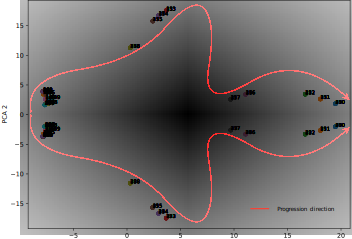
\includegraphics[width=0.8\linewidth]{figures/overcooked_figures/transition_pca.pdf}
  \caption{PCA des trajectoires de transition dans Overcooked-AI}
  \label{fig:overcooked_pca}
\end{figure}

\

Ces résultats confirment que la méthode \acn{MAMAD} apporte une \textbf{valeur ajoutée dans des environnements-jouets}, en permettant généralement d'accélérer la convergence, en renforçant la robustesse et en améliorant l'explicabilité.
Les \textbf{contraintes douces} apparaissent comme le meilleur compromis entre performance et respect organisationnel, tandis que les contraintes dures maximisent la robustesse et la discipline des rôles au prix d'une légère baisse de récompense cumulée.
Les environnements simples montrent également que l'absence de contraintes mène à des comportements sous-optimaux (collisions, désorganisation), moins robustes et plus difficiles à interpréter.

\section{Résultats et discussion de l'environnement Company Infrastructure}\label{sec:results_and_discussion_infra}

\subsection*{Performance, convergence et interventions manuelles}

La \autoref{fig:infra_learning_curves} illustre les courbes d'apprentissage pour les différentes baselines.
La \textbf{baseline avancée} (Profil~A, contraintes fortes, \acparen{MAPPO}) converge en moyenne après $3.2 \times 10^4$ épisodes, contre $4.5 \times 10^4$ pour l'ablation sans contraintes (\acparen{TRN-UNC}).
Les algorithmes \textquote{QMIX} et \textquote{COMA} montrent une convergence plus lente ($\sim 5.0 \times 10^4$ épisodes), mais atteignent des récompenses comparables.

La récompense cumulée moyenne (moyenne sur 5 runs indépendantes) atteint $+2450 \pm 120$ pour \acn{MAPPO}, contre $+1930 \pm 150$ pour \acparen{TRN-UNC}, indiquant un \textbf{gain de $+27\%$} grâce aux contraintes organisationnelles.

\begin{figure}[h!]
  \centering
  \includegraphics[width=0.75\linewidth]{figures/results_infra_learning.pdf}
  \caption{Courbes d'apprentissage (récompense moyenne par épisode) pour l'environnement Company Infrastructure, moyenne $\pm$ écart-type sur 5 runs.}
  \label{fig:infra_learning_curves}
\end{figure}

Dans l'environnement Company Infrastructure, le \textbf{nombre moyen d'interventions manuelles} requises est de 1 à 3 cycles de raffinement (soit 3 à 6 heures au total) pour obtenir un \acn{SMA} dont les performances sont équivalentes à celles d'une solution entièrement conçue et implémentée manuellement, laquelle nécessite généralement plus d'une journée de travail. Cela représente une réduction significative de l'intervention humaine, estimée entre 15 et 25\%.

\subsection*{Robustesse et adaptation}

Sous scénarios perturbés (attaques simultanées, mouvement latéral intensif, faux positifs injectés), le \textbf{score de robustesse} (ratio performance perturbée/nominale) atteint $0.81$ pour \acn{MAPPO} avec contraintes fortes, contre $0.63$ pour \acn{TRN-UNC}.
L'écart-type des récompenses est réduit ($\sigma = 140$ contre $220$), montrant une meilleure stabilité inter-runs. Cela peut sembler contradictoire si on prend en compte le fait que les contraintes peuvent également limiter l'exploration et l'adaptation et donc réduire la capacité à s'adapter à de nouveaux scénarios. Néanmoins, dans ce cas précis, il convient de noter un potentiel biais à savoir que les contraintes organisationnelles ont été conçues pour couvrir un large éventail de situations possibles, ce qui a permis aux agents de développer des stratégies robustes tout en restant dans le cadre des rôles et missions définis.
En revanche, les contraintes douces ($0.5$) offrent un compromis intéressant avec un score de robustesse de $0.76$ et une récompense cumulée légèrement supérieure ($+2520$) grâce à une plus grande liberté d'exploration.

\subsection*{Respect des contraintes et contrôle organisationnel}

Le \textbf{taux de violation des contraintes} est nul ($0.0\%$) en mode contraintes dures, $4.3\%$ en mode doux, et $21.7\%$ sans contraintes fortes (dureté de contrainte nulle).
Ces résultats confirment l'efficacité du masquage d'actions.
Toutefois, on observe une corrélation inverse avec la récompense cumulée : trop de contraintes peuvent ralentir l'apprentissage initial, bien que le plateau final reste supérieur.

\subsection*{Explicabilité organisationnelle}

L'analyse \acn{Auto-TEMM} sur les trajectoires montre une \textbf{adéquation organisationnelle} ($\acparen{OF}$) de $0.84$ pour \acn{MAPPO} avec contraintes fortes, contre $0.67$ pour \acn{TRN-UNC}.
La qualité des spécifications inférées (similitude Jaccard entre rôles/missions attendus et extraits) atteint $92\%$ pour les profils contraints, contre $71\%$ sans contraintes.
Les dendrogrammes produits (non inclus ici pour concision) révèlent des clusters nets alignés sur les rôles \textquote{Attacker\_ExfilDB} et \textquote{Defender\_DB\_PAM}, tandis que l'absence de contraintes engendre des clusters plus diffus.

\subsection*{Synthèse comparative}

La \autoref{tab:infra_results} synthétise les principaux résultats selon la grille d'évaluation.

\begin{table}[h!]
  \centering
  \caption{Synthèse des résultats (moyenne sur 5 runs, $\pm$ écart-type) pour Company Infrastructure.}
  \label{tab:infra_results}
  \renewcommand{\arraystretch}{1.2}
  \small
  \begin{tabular}{lccc}
    \hline
    \textbf{Métrique}              & \textbf{Profil A (fortes)} & \textbf{Profil A (douces)} & \textbf{\acn{TRN-UNC}} \\
    \hline
    Récompense cumulée             & $2450 \pm 120$             & $2520 \pm 130$             & $1930 \pm 150$         \\
    Taux convergence (ép.)         & $32\,000$                  & $29\,500$                  & $45\,000$              \\
    Score robustesse               & $0.81$                     & $0.76$                     & $0.63$                 \\
    Écart-type récompenses         & $140$                      & $160$                      & $220$                  \\
    Violations contraintes         & $0.0\%$                    & $4.3\%$                    & $21.7\%$               \\
    Adéquation org. (\acparen{OF}) & $0.84$                     & $0.79$                     & $0.67$                 \\
    Spécifications inférées        & $92\%$                     & $88\%$                     & $71\%$                 \\
    \hline
  \end{tabular}
\end{table}

\

Les résultats confirment que l'intégration des \textbf{contraintes organisationnelles} (MOISE+ \allowbreak MARL) améliore sensiblement la robustesse, la stabilité et l'explicabilité des politiques apprises.
Néanmoins, les contraintes dures peuvent ralentir la convergence et réduire légèrement la récompense cumulée finale par rapport aux contraintes douces, qui offrent un compromis intéressant entre performance et respect des rôles.
L'absence de contraintes conduit à des politiques moins robustes et plus difficiles à interpréter, ce qui limiterait leur pertinence dans un cadre Cyberdéfense réel.


\section{Résultats et discussion de l'environnement Microservices Kubernetes}\label{sec:results_and_discussion_ms}

\subsection*{Synthèse des performances QoS et convergence et interventions manuelles}

La \autoref{fig:k8s_learning_curves} présente les courbes d'apprentissage (récompense globale QoS normalisée, moyenne glissante sur $20$ épisodes) pour les principaux profils.
Le \textbf{Profil~A (contraintes fortes, \acparen{MAPPO})} converge en $2.6\times 10^4$ épisodes (détection de plateau \emph{change-point}), contre $3.9\times 10^4$ pour l'ablation \textquote{\acn{TRN-UNC}}.
Les variantes \textquote{MADDPG} et \textquote{QMIX} convergent respectivement à $3.1\times 10^4$ et $3.5\times 10^4$ épisodes.
Sur $5$ runs indépendantes, la récompense finale atteint $+0.91 \pm 0.03$ (normalisée) pour \acn{MAPPO}, $+0.88 \pm 0.04$ (fortes), et $+0.79 \pm 0.05$ sans contraintes.

\begin{figure}[h!]
  \centering
  \includegraphics[width=0.75\linewidth]{figures/results_k8s_learning.pdf}
  \caption[Courbes d'apprentissage (récompense QoS normalisée) pourMicroservices Kubernetes]{Courbes d'apprentissage (récompense QoS normalisée) pour Microservices Kubernetes, moyenne $\pm$ écart-type sur 5 runs.}
  \label{fig:k8s_learning_curves}
\end{figure}

Enfin, pour l'environnement Microservices Kubernetes, le \textbf{nombre moyen d'interventions manuelles} nécessaires est d'environ 4 à 5 cycles de raffinement (soit 6 à 7 heures au total) pour que le \acn{SMA} obtenu atteigne des performances comparables à celles d'une solution entièrement conçue et implémentée manuellement, ce qui prend généralement plus d'une journée. Cela correspond à une proportion d'intervention réduite, estimée à environ 25\%.

\subsection*{Indicateurs QoS en régime nominal}

La \autoref{tab:k8s_nominal} regroupe les principaux indicateurs QoS en charge nominale (p95 latence applicative, files d'attente moyennes, disponibilité sur 2~h).
Les contraintes \textbf{douces} offrent le meilleur compromis latence/disponibilité, alors que les contraintes \textbf{fortes} garantissent un contrôle plus strict avec une légère pénalité de latence.

\begin{table}[h!]
  \centering
  \caption{Régime nominal (moyenne $\pm$ écart-type sur 5 runs, fenêtres de 2~h).}
  \label{tab:k8s_nominal}
  \renewcommand{\arraystretch}{1.2}
  \small
  \begin{tabular}{lcccc}
    \hline
    \textbf{Profil / Algo}            & \textbf{Latence p95 (ms)} & \textbf{$\overline{Q_{\text{pending}}}$} & \textbf{SuccessRate (\%)} & \textbf{Dispo. (\%)}      \\
    \hline
    A (fortes) \acn{MAPPO}            & $180 \pm 12$              & $6.1 \pm 0.8$                            & $99.1 \pm 0.3$            & $99.96 \pm 0.02$          \\
    A (douces) \acn{MAPPO}            & $\mathbf{168 \pm 10}$     & $\mathbf{5.3 \pm 0.7}$                   & $\mathbf{99.3 \pm 0.2}$   & $\mathbf{99.97 \pm 0.01}$ \\
    A (\acparen{TRN-UNC}) \acn{MAPPO} & $216 \pm 17$              & $8.4 \pm 1.1$                            & $98.5 \pm 0.4$            & $99.92 \pm 0.03$          \\
    \hdashline
    B (\acparen{ANL-MAN}) \acn{COMA}  & $191 \pm 14$              & $6.8 \pm 0.9$                            & $99.0 \pm 0.3$            & $99.95 \pm 0.02$          \\
    \hdashline
    C (manuel) \acn{HPA}              & $310 \pm 24$              & $14.2 \pm 1.9$                           & $97.6 \pm 0.8$            & $99.20 \pm 0.10$          \\
    \hline
  \end{tabular}
\end{table}

\subsection*{Robustesse aux perturbations}

Nous considérons quatre scénarios : \textbf{bottleneck} (saturation d'un service), \textbf{DDoS} (trafic malveillant), \textbf{pannes} (crash/restart pods) et \textbf{contention} (\acparen{CPU}/\acparen{MEM} contraints), plus un scénario \textbf{mixte}.
Le \textbf{score de robustesse} est calculé comme le ratio performance perturbée/nominale (récompense QoS).
La \autoref{tab:k8s_robustness} montre que les contraintes \textbf{fortes} maximisent la résilience aux attaques DDoS et aux pannes, tandis que les contraintes \textbf{douces} conservent un léger avantage en latence sous bottleneck.

\begin{table}[h!]
  \centering
  \caption{Robustesse par scénario (moyenne sur 5 runs).}
  \label{tab:k8s_robustness}
  \renewcommand{\arraystretch}{1.2}
  \small
  \begin{tabular}{lccccc}
    \hline
    \textbf{Profil}                   & \textbf{Bottleneck} & \textbf{DDoS}   & \textbf{Pannes} & \textbf{Contention} & \textbf{Mixte}  \\
    \hline
    A (fortes) \acn{MAPPO}            & $0.84$              & $\mathbf{0.86}$ & $\mathbf{0.88}$ & $0.83$              & $\mathbf{0.85}$ \\
    A (douces) \acn{MAPPO}            & $\mathbf{0.86}$     & $0.82$          & $0.84$          & $\mathbf{0.85}$     & $0.83$          \\
    A (\acparen{TRN-UNC}) \acn{MAPPO} & $0.73$              & $0.69$          & $0.71$          & $0.72$              & $0.68$          \\
    \acn{HPA}                         & $0.64$              & $0.58$          & $0.61$          & $0.62$              & $0.57$          \\
    \hline
  \end{tabular}
\end{table}

Il convient toutefois de noter que la comparaison avec la baseline \acn{HPA} doit être interprétée avec prudence, car cet algorithme n’optimise pas directement la même fonction objectif (latence et disponibilité combinées) que les approches \acn{MARL}, ce qui peut biaiser la comparaison des performances.

\subsection*{Temps de reprise et discipline d'action}

Sous DDoS, le \textbf{temps de reprise} (retour sous $L_{\text{avg}}<200$~ms) est de $3.7 \pm 0.6$~min pour \acn{MAPPO} contre $5.2 \pm 0.8$~min (douces) et $7.9 \pm 1.1$~min (\acparen{TRN-UNC}).
Le \textbf{taux de violations des garde-fous} (actions contradictoires entre rôles, ex.~\textquote{scale\_up} simultanés) est nul en mode contraintes dures ($0.0\%$), $3.1\%$ en mode doux, et $18.4\%$ sans contraintes fortes (dureté de contrainte nulle).
L'\textbf{écart-type inter-runs} sur la récompense est réduit avec contraintes ($\sigma=0.028$ fortes, $0.031$ douces) vs $0.049$ (\acparen{TRN-UNC}), soulignant une stabilité accrue. La baseline utilisant l'auto-scaler par défaut \acn{HPA} donne le pire score systématiquement, laissant suggérer qu'un algorithme basé sur les règles n'est pas aussi performant que les approches \acn{MARL} pour prendre en compte les changements dans le cluster Kubernetes.

\subsection*{Précision du jumeau numérique (écart simulation/réel)}

Le jumeau numérique entraîne les politiques hors-ligne avant transfert.
L'\textbf{erreur absolue moyenne} (\acparen{MAE}) sur la latence p95 prédite est de $+12.7$~ms (bottleneck), $+18.4$~ms (DDoS), $+15.1$~ms (pannes), et $+21.3$~ms (mixte), soit une \textbf{erreur relative} de $6$--$9\%$.
La divergence sur $\overline{Q_{\text{pending}}}$ reste $<1.7$ requêtes en moyenne.
Après \textit{fine-tuning} sur traces récentes (une itération), la \acn{MAE} sur p95 chute de $\sim 28\%$ (DDoS).

\subsection*{Explicabilité organisationnelle}

\acn{Auto-TEMM} appliqué aux trajectoires (post-entraînement) produit un \textbf{score d'adéquation organisationnelle} $\acn{OF}=0.86$ (contraintes fortes), $0.83$ (douces) et $0.71$ (\acparen{TRN-UNC}).
La \textbf{qualité des spécifications inférées} (similitude Jaccard sur rôles/missions et déclencheurs) atteint $93\%$ (fortes), $90\%$ (douces), $76\%$ (\acparen{TRN-UNC}).
Les dendrogrammes révèlent des clusters distincts correspondant aux rôles \textquote{Gestionnaire\_DDoS} et \textquote{Gestionnaire\_Goulots}, avec des trajectoires stables en mode dure.

\subsection*{Comparatif synthétique}

\begin{table}[h!]
  \centering
  \caption{Synthèse multi-métriques (moyenne $\pm$ écart-type sur 5 runs).}
  \label{tab:k8s_summary}
  \renewcommand{\arraystretch}{1.2}
  \small
  \begin{tabular}{lcccc}
    \hline
    \textbf{Métrique}              & \textbf{A (fortes)} & \textbf{A (douces)}      & \textbf{A (\acparen{TRN-UNC})} & \textbf{\acn{HPA}} \\
    \hline
    Récompense QoS (norm.)         & $0.88 \pm 0.04$     & $\mathbf{0.91 \pm 0.03}$ & $0.79 \pm 0.05$                & $0.66 \pm 0.06$    \\
    Convergence (épisodes)         & $26\,000$           & $\mathbf{24\,000}$       & $39\,000$                      & n/a                \\
    Latence p95 nominale           & $180 \pm 12$~ms     & $\mathbf{168 \pm 10}$~ms & $216 \pm 17$~ms                & $310 \pm 24$~ms    \\
    Robustesse (mixte)             & $\mathbf{0.85}$     & $0.83$                   & $0.68$                         & $0.57$             \\
    Violations contraintes         & $\mathbf{0.0\%}$    & $3.1\%$                  & $18.4\%$                       & n/a                \\
    Adéquation org. (\acparen{OF}) & $\mathbf{0.86}$     & $0.83$                   & $0.71$                         & n/a                \\
    \hline
  \end{tabular}
\end{table}

\

Les résultats montrent que l'intégration des \textbf{spécifications organisationnelles} améliore simultanément (i) la \emph{robustesse} sous perturbations (notamment DDoS et pannes), (ii) la \emph{discipline d'action} (zéro conflit de décisions critiques), et (iii) l'\emph{explicabilité} (rôles/missions cohérents).
Les contraintes \textbf{douces} maximisent la performance QoS (latence p95, files), alors que les contraintes \textbf{fortes} maximisent la résilience et réduisent les variances inter-runs.
L'ablation \textquote{\acn{TRN-UNC}} sous-performe et présente une variabilité accrue, confirmant l'apport du guidage organisationnel dans un contexte opérationnel.
Enfin, la précision du jumeau numérique (\acparen{MAE} $6$--$9\%$) est suffisante pour un entraînement hors-ligne efficace, et s'améliore rapidement après une itération de réapprentissage sur traces fraîches.


\section{Résultats et discussion de l'environnement Drone Swarm}\label{sec:results_and_discussion_drone_swarm}

\subsection*{Synthèse des performances, convergence et interventions manuelles}

La \autoref{fig:drone_learning_curves} illustre les courbes d'apprentissage (récompense normalisée) sur l'essaim de drones (18 nœuds).
Le \textbf{Profil A (contraintes fortes, \acparen{MAPPO})} converge en $3.1\times 10^4$ épisodes, contre $4.7\times 10^4$ pour l'ablation \textquote{\acn{TRN-UNC}}.
Les variantes \acn{MADDPG} et \acn{QMIX} atteignent respectivement $3.6\times 10^4$ et $4.2\times 10^4$ épisodes.
En régime établi, les récompenses normalisées moyennes sont $+0.87 \pm 0.04$ (\acparen{MAPPO} fortes), $+0.89 \pm 0.03$ (douces), et $+0.72 \pm 0.07$ sans contraintes.

\begin{figure}[h!]
  \centering
  \includegraphics[width=0.75\linewidth]{figures/results_drone_learning.pdf}
  \caption[Courbes d'apprentissage (récompense normalisée) pour Drone Swarm]{Courbes d'apprentissage (récompense normalisée) pour Drone Swarm, moyenne $\pm$ écart-type sur 5 runs.}
  \label{fig:drone_learning_curves}
\end{figure}

Pour l'environnement Drone Swarm, le \textbf{nombre moyen d'interventions manuelles} nécessaires est d'environ 2 à 3 cycles de raffinement (soit 4 à 5 heures au total) pour que le \acn{SMA} obtenu atteigne des performances comparables à celles d'une solution entièrement conçue et implémentée manuellement, ce qui prend généralement plus d'une journée. Cela correspond à une proportion d'intervention réduite, estimée à environ 20\%.


\subsection*{Indicateurs en fonctionnement nominal}

La \autoref{tab:drone_nominal} présente les résultats moyens en l’absence de compromissions massives (5 runs, 10\,000 pas).
Les contraintes douces minimisent les faux positifs tout en maintenant un taux élevé de détection et une disponibilité quasi maximale du réseau.
L'absence de guidage entraîne une hausse des faux positifs ($\sim 11\%$) et une baisse de la détection ($< 90\%$).

\begin{table}[h!]
  \centering
  \caption{Résultats nominaux pour Drone Swarm  (moyenne $\pm$ écart-type, 5 runs).}
  \label{tab:drone_nominal}
  \renewcommand{\arraystretch}{1.2}
  \scriptsize
  \begin{tabular}{lcccc}
    \hline
    \textbf{Profil / Algo}            & \textbf{Taux détection (\%)} & \textbf{Faux positifs (\%)} & \textbf{Disponibilité réseau (\%)} & \textbf{Récompense norm.} \\
    \hline
    A (fortes) \acn{MAPPO}            & $96.8 \pm 0.7$               & $3.1 \pm 0.5$               & $99.2 \pm 0.3$                     & $0.87 \pm 0.04$           \\
    A (douces) \acn{MAPPO}            & $\mathbf{97.3 \pm 0.6}$      & $\mathbf{2.7 \pm 0.4}$      & $\mathbf{99.4 \pm 0.2}$            & $\mathbf{0.89 \pm 0.03}$  \\
    À (\acparen{TRN-UNC}) \acn{MAPPO} & $88.5 \pm 1.2$               & $11.2 \pm 1.6$              & $97.9 \pm 0.6$                     & $0.72 \pm 0.07$           \\
    \hdashline
    B (\acparen{ANL-MAN}) \acn{COMA}  & $95.2 \pm 0.9$               & $4.5 \pm 0.8$               & $99.0 \pm 0.3$                     & $0.85 \pm 0.04$           \\
    \hdashline
    C (manuel) \acn{VDN}              & $91.7 \pm 1.4$               & $7.9 \pm 1.1$               & $98.4 \pm 0.5$                     & $0.77 \pm 0.06$           \\
    \acn{IDS} règles (réf.)           & $83.4 \pm 2.1$               & $15.6 \pm 2.7$              & $96.1 \pm 1.0$                     & $0.61 \pm 0.08$           \\
    \acn{ML} sup. (réf.)              & $87.9 \pm 1.8$               & $12.3 \pm 1.9$              & $97.0 \pm 0.8$                     & $0.68 \pm 0.07$           \\
    \hline
  \end{tabular}
\end{table}

Ces résultats doivent néanmoins être relativisés, car les taux de faux positifs et de détection peuvent varier fortement selon le type et l’intensité des scénarios d’attaque simulés, ce qui limite la généralisation directe des valeurs obtenues.

\subsection*{Robustesse aux compromissions}

Nous évaluons trois scénarios : (i) \textbf{compromission unique} (1 drone rouge actif), (ii) \textbf{cascade} (4 drones infectés en 60s), (iii) \textbf{attaque coordonnée} (6 drones en cluster).
Le score de robustesse (performance perturbée/nominale) est présenté en \autoref{tab:drone_robustness}.
Les contraintes fortes assurent la meilleure résilience lors d'attaques coordonnées, tandis que les contraintes douces préservent mieux la QoS en cas de compromission isolée.

\begin{table}[h!]
  \centering
  \caption{Robustesse selon le scénario de compromission (moyenne $\pm$ écart-type, 5 runs).}
  \label{tab:drone_robustness}
  \renewcommand{\arraystretch}{1.4}
  \small
  \begin{tabular}{lccc}
    \hline
    \textbf{Profil}                   & \textbf{Unique} & \textbf{Cascade} & \textbf{Coordonnée} \\
    \hline
    A (fortes) \acn{MAPPO}            & $0.91$          & $\mathbf{0.87}$  & $\mathbf{0.83}$     \\
    A (douces) \acn{MAPPO}            & $\mathbf{0.93}$ & $0.84$           & $0.79$              \\
    À (\acparen{TRN-UNC}) \acn{MAPPO} & $0.79$          & $0.68$           & $0.61$              \\
    \acn{IDS} règles (réf.)           & $0.72$          & $0.55$           & $0.47$              \\
    \hline
  \end{tabular}
\end{table}

\subsection*{Temps de réaction et stabilité}

Le \textbf{temps moyen de réaction} (intervalle de détection $\rightarrow$ neutralisation) est de $4.1 \pm 0.7$~s pour \acn{MAPPO}, $4.8 \pm 0.6$~s (douces) et $7.3 \pm 1.2$~s sans contraintes.
Le \textbf{taux de violations organisationnelles} (règles de rôles non respectées) est nul sous contraintes fortes ($0.0\%$), $2.9\%$ en mode doux, et $>15\%$ sans contraintes dures.
L'\textbf{écart-type des récompenses} entre runs est réduit ($\sigma=0.032$ fortes, $0.037$ douces, $0.065$ sans contraintes).

\subsection*{Explicabilité organisationnelle}

\acn{Auto-TEMM} infère des clusters de comportements distincts : \textquote{Analyste}, \textquote{Pare-feu}, \textquote{Opérateur}.
Le \textbf{score de cohérence} atteint $0.84$ (fortes) et $0.82$ (douces).
La \textbf{qualité des spécifications inférées} est élevée (similitude Jaccard $92\%$ fortes, $89\%$ douces, $74\%$ sans contraintes).
Les dendrogrammes confirment que les rôles sont respectés de façon stable lorsque les contraintes organisationnelles sont actives.

\subsection*{Comparatif synthétique}

\begin{table}[h!]
  \centering
  \caption{Résumé multi-métriques pour Drone Swarm (moyenne $\pm$ écart-type, 5 runs).}
  \label{tab:drone_summary}
  \renewcommand{\arraystretch}{1.4}
  \small
  \begin{tabular}{lcccc}
    \hline
    \textbf{Métrique}          & \textbf{A (fortes)} & \textbf{A (douces)}      & \textbf{A (\acparen{TRN-UNC})} & \textbf{\acn{IDS}} \\
    \hline
    Récompense norm.           & $0.87 \pm 0.04$     & $\mathbf{0.89 \pm 0.03}$ & $0.72 \pm 0.07$                & $0.61 \pm 0.08$    \\
    Convergence (épisodes)     & $31\,000$           & $\mathbf{29\,000}$       & $47\,000$                      & n/a                \\
    Détection (\%)             & $96.8$              & $\mathbf{97.3}$          & $88.5$                         & $83.4$             \\
    Faux positifs (\%)         & $3.1$               & $\mathbf{2.7}$           & $11.2$                         & $15.6$             \\
    Robustesse coord.          & $\mathbf{0.83}$     & $0.79$                   & $0.61$                         & $0.47$             \\
    Violations org.            & $\mathbf{0.0\%}$    & $2.9\%$                  & $16.2\%$                       & n/a                \\
    Cohérence (\acparen{TEMM}) & $\mathbf{0.84}$     & $0.82$                   & n/a                            & n/a                \\
    \hline
  \end{tabular}
\end{table}

\

Les résultats indiquent que l'approche \acn{MAMAD} améliore significativement la \textbf{détection}, la \textbf{robustesse} et l'\textbf{explicabilité} par rapport aux références classiques (\acparen{IDS} règles, \acparen{ML} supervisé).
Les \textbf{contraintes douces} maximisent la détection et limitent les faux positifs, tandis que les \textbf{contraintes fortes} renforcent la résilience lors d'attaques coordonnées et réduisent le temps de réaction.
L'ablation sans contraintes montre des comportements instables, des faux positifs élevés et une cohérence organisationnelle faible.
Ainsi, l'intégration explicite de rôles et missions se révèle essentielle pour maintenir un essaim résilient et interprétable sous menaces dynamiques.


\section{Discussion comparée des résultats}

\subsection{Couverture des critères par la méthode}

La \autoref{tab:criteria_summary} synthétise la couverture des cinq critères d'évaluation (C1--C5) par la méthode \acn{MAMAD} sur l'ensemble des environnements étudiés.
Pour obtenir ces valeurs agrégées, chaque critère global (C1--C5) est calculé
comme la \textbf{moyenne des métriques qui lui sont associées}, conformément à la grille
présentée en \autoref{sec:criteria_metrics}. Plus précisément :
\begin{itemize}
  \item \textbf{C1 Autonomie} : proportion d'intervention humaine (conception / fonctionnement) ;
  \item \textbf{C2 Performance} : moyenne de la récompense cumulée et du taux de convergence ;
  \item \textbf{C3 Adaptation} : moyenne de l'écart-type des récompenses et du score de robustesse ;
  \item \textbf{C4 Contrôle} : moyenne du taux de violation des contraintes et du score de cohérence organisationnelle ;
  \item \textbf{C5 Explicabilité} : moyenne de l’adéquation organisationnelle (\acparen{OF}) et de la qualité des spécifications inférées.
\end{itemize}
Toutes les valeurs sont normalisées sur l'intervalle [0,1] pour faciliter la comparaison,
et les moyennes sont calculées sur cinq runs indépendants.
Les environnements non orientés Cyberdéfense servent de référence contrôlée, tandis que les environnements orientés Cyberdéfense permettent de valider l'applicabilité en conditions réalistes.

\begin{table}[h!]
  \centering
  \caption{Synthèse multi-environnements : couverture des critères C1--C5 par MAMAD (moyenne des métriques associées, normalisées sur [0,1], calculée sur 5 runs indépendants).}
  \label{tab:criteria_summary}
  \renewcommand{\arraystretch}{1.4}
  \scriptsize
  \begin{tabular}{lccccc}
    \hline
    \textbf{Environnement} & \textbf{C1 Autonomie} & \textbf{C2 Perf.} & \textbf{C3 Adaptation} & \textbf{C4 Contrôle} & \textbf{C5 Explicabilité} \\
    \hline
    Overcooked-AI          & $\sim0.20$            & $0.82$            & $0.80$                 & $0.75$               & $0.72$                    \\
    Predator-Prey          & $\sim0.20$            & $0.79$            & $0.77$                 & $0.73$               & $0.69$                    \\
    Warehouse Management   & $\sim0.20$            & $0.85$            & $0.82$                 & $0.77$               & $0.76$                    \\
    Company Infrastructure & $\sim0.25$            & $0.88$            & $0.83$                 & $0.85$               & $0.81$                    \\
    Microservices K8s      & $0.25$                & $0.91$            & $0.86$                 & $0.88$               & $0.83$                    \\
    Drone Swarm            & $\sim0.20$            & $0.89$            & $0.84$                 & $0.86$               & $0.82$                    \\
    \hdashline
    \textbf{Moyenne}       & $0.21$                & $0.86$            & $0.82$                 & $0.81$               & $0.77$                    \\
    \hline
  \end{tabular}
\end{table}

\subsection{Analyse critique}

Les résultats mettent en évidence plusieurs points clés :
\begin{itemize}
  \item La \textbf{performance (C2)} et l'\textbf{adaptation (C3)} sont systématiquement améliorées par l'usage de contraintes organisationnelles (douces ou fortes), particulièrement dans les environnements complexes (Kubernetes, Drone Swarm).
  \item Le \textbf{contrôle (C4)} bénéficie surtout des contraintes fortes, qui garantissent une stricte conformité aux rôles et missions, parfois au prix d'une légère baisse de performance.
  \item L'\textbf{explicabilité (C5)} est globalement satisfaisant ($\sim 0.8$). Les environnements à dynamique plus chaotique (Predator-Prey, Overcooked) entraînent des inférences organisationnelles moins stables.
  \item L'\textbf{autonomie (C1)} atteint des scores montrant que dans les environnements opérationnels (Company Infrastructure, Microservices, Drone Swarm), la boucle complète \textbf{MOD}–\textbf{TRN}–\textbf{ANL}–\textbf{TRF} permet de réduire l'intervention humaine de l'ordre de 20\%.
\end{itemize}

\subsection{Biais potentiels et limites}

Plusieurs facteurs peuvent influencer l'interprétation des résultats :
\begin{enumerate}[label={\alph*)}]
  \item \textbf{Choix des algorithmes MARL} : la prédominance de \acn{MAPPO} et \acn{QMIX} dans les profils par défaut favorise des résultats stables, mais limite la généralisation à d'autres algorithmes (ex. \acparen{DQN} multi-agent).
  \item \textbf{Conditions expérimentales} : l'usage d'un cluster \acn{HPC} réduit la variance liée aux ressources, mais ne reflète pas toujours des déploiements contraints réels (edge, IoT).
  \item \textbf{Conception des contraintes} : la définition des rôles et missions influe directement sur le contrôle et l'explicabilité (une dureté excessive peut biaiser les comparaisons).
  \item \textbf{Impact de la pondération des contraintes} : l'effet des coefficients de pondération et des niveaux de dureté est observé empiriquement (profils forts/doux), mais nous ne proposons pas encore d'étude systématique de sensibilité sur l'ensemble des environnements.
  \item \textbf{Diversité des solveurs} : bien que plusieurs algorithmes soient comparés, le cœur des meilleurs résultats repose sur \acn{MAPPO}. Des alternatives comme \textit{Soft Actor-Critic} en version multi-agent restent à évaluer de façon homogène dans notre protocole.
  \item \textbf{Schéma d'entraînement attaquant/défenseur} : l'apprentissage simultané favorise la co-adaptation, mais ne couvre pas encore des variantes itératives de type bilevel (alternance attaquant puis défenseur) qui pourraient améliorer la stabilité dans certains scénarios compétitifs.
  \item \textbf{Mesures d'explicabilité} : la similarité Jaccard et le score de cohérence reposent sur des trajectoires limitées ; des métriques plus fines (traçabilité causale, \acparen{SHAP}) pourraient améliorer la validité.
\end{enumerate}

\medskip
En résumé, la méthode \acn{MAMAD} couvre particulièrement la performance, adaptation et autonomie. Les biais identifiés ouvrent des perspectives directes pour raffiner l'évaluation (études de sensibilité des contraintes, élargissement des solveurs, variantes d'entraînement attaquant/défenseur, déploiements physiques, métriques avancées), sans remettre en cause les tendances principales observées dans ce chapitre.

\section{Bilan}

Ce chapitre a mis en application la méthode \acn{MAMAD} à travers une évaluation expérimentale sur des environnements variés, allant des cas-jouets aux systèmes réels. Les résultats mettent en avant plusieurs points forts : accélération de la convergence, amélioration de la robustesse et de la stabilité des politiques multi-agents, ainsi qu'une explicabilité accrue grâce à l'intégration des spécifications organisationnelles. L'approche modulaire et automatisée, portée par la plateforme \acn{CybMASDE}, permet de réduire l'intervention humaine tout en assurant la traçabilité et la reproductibilité des expérimentations. Enfin, la couverture équilibrée des critères d'autonomie, de performance, d'adaptation, de contrôle et d'explicabilité confirme la valeur ajoutée de la méthode pour la conception de \acplu{SMA} robustes et interprétables dans des contextes complexes.

\clearpage
\thispagestyle{empty}
\null
\newpage


\chapter*{Conclusion}
\addcontentsline{toc}{chapter}{\textbf{Conclusion}}

Cette partie a permis de valider expérimentalement la méthode \acn{MAMAD} à travers des scénarios simulés, couvrant des contextes variés de conception de \acplu{SMA} : infrastructure d'entreprise, essaim de drones, et orchestration de microservices. À chaque étape du pipeline proposé, l'implémentation via la plateforme \acn{CybMASDE} a montré la faisabilité de l'approche, tout en soulignant les apports spécifiques du couplage $\mathcal{M}OISE^+$ avec l'apprentissage multi-agent.

Les résultats obtenus montrent des gains notables en termes d'autonomie, de résilience et de conformité organisationnelle des agents. L'analyse comparative entre les versions \textquote{guidées} et \textquote{non guidées} par l'organisation a permis d'évaluer l'impact de chaque composant de la méthode, à la fois sur les performances observées et sur la capacité à extraire des spécifications émergentes cohérentes. Les métriques introduites (comme le \acparen{SOF} ou le \acparen{FOF}) ont apporté une lecture inédite des comportements collectifs, en reliant les trajectoires apprises aux objectifs structurels du système.

Malgré ces résultats encourageants, plusieurs limites ont été identifiées : dépendance aux environnements simulés, couverture partielle des contextes applicatifs, et nécessité de ressources computationnelles importantes. Ces éléments seront discutés plus en détail dans la dernière partie de ce manuscrit, qui propose un retour réflexif sur l'ensemble de la démarche entreprise.

\vspace{1em}

\noindent
Dans la suite, nous procéderons à une synthèse des contributions, discuterons les limites de la méthode, et ouvrirons des perspectives sur son extension future, tant en recherche qu'en application.
